\documentclass[12pt]{article}
\usepackage[a4paper, total={21cm, 29.7cm}, margin=3cm]{geometry}
\usepackage[paper=A4]{typearea}
\usepackage{times}    % times new roman font
\usepackage{amsmath}
\usepackage{listings} % cool ah code
\usepackage{color}    % more cool shit code
\usepackage{graphicx} % fancy ah figure
\usepackage{float}    % forcing figure to float
\usepackage{enumitem}
\usepackage{lipsum} % sampling
\usepackage{setspace}
% \usepackage{mdframed}
\usepackage{indentfirst} 
\usepackage[hidelinks]{hyperref} % actually used for email and links, but kinda broken. (not used)
\usepackage{tabularx} % just because, but now more often use longtable
\usepackage{longtable} % cool table with it speciality to be able cut along 2 page
\usepackage{multirow} % merge row
\usepackage[titles]{tocloft} % table of content
\usepackage{rotating} % rotating figure
\usepackage[tableposition=top]{caption} % need to explain?
\usepackage[none]{hyphenat} % no linebreak with -
% \usepackage{showframe} % debugging
\usepackage{natbib} % bib cite stuff
\usepackage{chngcntr} % change counter
\usepackage{afterpage} % change counter
\usepackage{pdflscape}

% \usepackage{cite}
% \bibliographystyle{abbrvnat}
\setcitestyle{open={(},close={)}} %Citation-related commands
\setlistdepth{9}

\newlist{exenumerate}{enumerate}{9}
\setlist[exenumerate,1]{label=\alph*}
\setlist[exenumerate,2]{label=(\Roman*)}
\setlist[exenumerate,3]{label=(\Alph*)}
\setlist[exenumerate,4]{label=(\roman*)}
\setlist[exenumerate,5]{label=(\alph*)}
\setlist[exenumerate,6]{label=\Alph*}
\setlist[exenumerate,7]{label=(\Roman*)}
\setlist[exenumerate,8]{label=(\Alph*)}
\setlist[exenumerate,9]{label=(\roman*)}

\usepackage{titlesec}



% Customize TOC
\renewcommand{\cftsecfont}{\bfseries}
\renewcommand{\cftsecpagefont}{\bfseries}
\renewcommand{\cftsubsecfont}{}
\renewcommand{\cftsubsecpagefont}{}
\renewcommand{\cftsubsubsecfont}{}
\renewcommand{\cftsubsubsecpagefont}{}


% Add dot leaders
\renewcommand{\cftpartleader}{\cftdotfill{\cftdotsep}}
\renewcommand{\cftsecleader}{\cftdotfill{\cftdotsep}}
\renewcommand{\cftsubsecleader}{\cftdotfill{\cftdotsep}}


\setlength{\cftbeforesecskip}{0.5em}
\setlength{\cftbeforesubsecskip}{0.5em}
\setlength{\cftbeforesubsubsecskip}{0.5em}

% Customize section numbering
\renewcommand\thesection{\arabic{section}}
\renewcommand\thesubsection{\thesection.\arabic{subsection}}
\renewcommand\thesubsubsection{\thesubsection.\arabic{subsubsection}}

% Customize section formatting
\titleformat{\section}[block]{\large\bfseries\filcenter}{}{0em}{}
\titleformat{\subsection}[hang]{\bfseries}{}{1em}{}
% \titleformat{\section}{\normalfont\Large\bfseries}{BAB \Roman{section}}{1em}{}
% \titleformat{\subsection}{\normalfont\large\bfseries}{\thesubsection}{1em}{}
% \titleformat{\subsubsection}{\normalfont\normalsize\bfseries}{\thesubsubsection}{1em}{}


\DeclareCaptionLabelFormat{nospace}{#1#2}
\captionsetup[table]{name=Tabel }
\captionsetup[figure]{name=Gambar }
\renewcommand{\thefigure}{\thesection.\arabic{figure}}
\renewcommand{\thetable}{\thesection.\arabic{table}}

% \usepackage[titles]{tocloft}
% \setlength{\cftbeforeloftitleskip}{0em} % Adjust spacing if necessary
% \setlength{\cftbeforelottitleskip}{0em}

\renewcommand{\refname}{DAFTAR PUSTAKA}
\renewcommand{\contentsname}{\centering DAFTAR ISI}
\renewcommand{\listfigurename}{\centering DAFTAR GAMBAR}
\renewcommand{\listtablename}{\centering DAFTAR TABEL}

\usepackage{etoolbox}
\patchcmd{\listoffigures}{\section*}{\section*{\centering}}{}{}
\patchcmd{\listoftables}{\section*}{\section*{\centering}}{}{}

% for list
\setlist{  
  listparindent=\parindent,
  parsep=0pt,
}
\newcommand{\listsection}[1]{
    \item \textbf{#1}
    \addcontentsline{toc}{subsection}{#1}
}


\setlength\parindent{2.5em}
\setlength{\emergencystretch}{2.5em}

\renewcommand{\baselinestretch}{1.2}
\renewcommand*{\arraystretch}{1.2} 
\setlength{\extrarowheight}{.2ex}

\definecolor{dkgreen}{rgb}{0,0.6,0}
\definecolor{gray}{rgb}{0.5,0.5,0.5}
\definecolor{mauve}{rgb}{0.58,0,0.82}

\lstset{frame=tb,
    language=Python,
    aboveskip=3mm,
    belowskip=3mm,
    showstringspaces=true,
    columns=flexible,
    basicstyle={\small\ttfamily},
    numbers=none,
    numberstyle=\tiny\color{gray},
    keywordstyle=\color{blue},
    commentstyle=\color{dkgreen},
    stringstyle=\color{mauve},
    breaklines=true,
    breakatwhitespace=true,
    tabsize=4
}

\def\mynewrule#1{\hbox to #1in{\leaders\hbox to 0.00625in{\hfil.\hfil}\hfill}}
%%%%Defined the signature line with \hfill%%%   
\def\rnewrule#1{\hfill\mynewrule{#1}}
%%%%Defined block to include rule and information%%%
\def\rsignblock#1#2{
    \hfill
    \vtop{
        \hsize=#1in
        \noindent{Semarang, ...}\par
        \vspace*{2cm}
        \noindent{#2}\par
    }
    \par
    \hfill
    % \rnewrule{#1}\par     
    \vskip1cm
}

\begin{document}
\begin{titlepage}
    \begin{center}
        {
            % \setstretch{2}
            \textbf{ LAPORAN PRAKTEK KERJA LAPANGAN} \\
            \textbf{SISTEM MANAJEMEN PRODUK DAN TICKETING}\\
            \textbf{ BAGIAN MODUL TICKETING} \\
            \textbf{DI PT TEKNOLOGI APLIKASI SEJAHTERA} \\
        }

        \vfill
        
\includegraphics[width=4cm]{images/logo-undip.png} \\
        \vfill
        \textbf{ Disusun Oleh:} \\
        Givandra Haikal Adjie \\
        240601211130063 \\

        \vspace{1cm}
        \textbf{
        DEPARTEMEN NFORMATIKA \\
        FAKULTAS SAINS DAN MATEMATIKA \\
        UNIVERSITAS DIPONEGORO \\
        SEMARANG \\
        2023}

    \end{center}
\end{titlepage}



% HALAMAN PENGESAHAN
%  ██      ██     ██     ██           ██     ████     ████     ██     ████     ██
% ░██     ░██    ████   ░██          ████   ░██░██   ██░██    ████   ░██░██   ░██
% ░██     ░██   ██░░██  ░██         ██░░██  ░██░░██ ██ ░██   ██░░██  ░██░░██  ░██
% ░██████████  ██  ░░██ ░██        ██  ░░██ ░██ ░░███  ░██  ██  ░░██ ░██ ░░██ ░██
% ░██░░░░░░██ ██████████░██       ██████████░██  ░░█   ░██ ██████████░██  ░░██░██
% ░██     ░██░██░░░░░░██░██      ░██░░░░░░██░██   ░    ░██░██░░░░░░██░██   ░░████
% ░██     ░██░██     ░██░████████░██     ░██░██        ░██░██     ░██░██    ░░███
% ░░      ░░ ░░      ░░ ░░░░░░░░ ░░      ░░ ░░         ░░ ░░      ░░ ░░      ░░░
%  ███████  ████████ ████     ██   ████████  ████████  ████████     ██      ██      ██     ██     ████     ██
% ░██░░░░██░██░░░░░ ░██░██   ░██  ██░░░░░░██░██░░░░░  ██░░░░░░     ████    ░██     ░██    ████   ░██░██   ░██
% ░██   ░██░██      ░██░░██  ░██ ██      ░░ ░██      ░██          ██░░██   ░██     ░██   ██░░██  ░██░░██  ░██
% ░███████ ░███████ ░██ ░░██ ░██░██         ░███████ ░█████████  ██  ░░██  ░██████████  ██  ░░██ ░██ ░░██ ░██
% ░██░░░░  ░██░░░░  ░██  ░░██░██░██    █████░██░░░░  ░░░░░░░░██ ██████████ ░██░░░░░░██ ██████████░██  ░░██░██
% ░██      ░██      ░██   ░░████░░██  ░░░░██░██             ░██░██░░░░░░██ ░██     ░██░██░░░░░░██░██   ░░████
% ░██      ░████████░██    ░░███ ░░████████ ░████████ ████████ ░██     ░██ ░██     ░██░██     ░██░██    ░░███
% ░░       ░░░░░░░░ ░░      ░░░   ░░░░░░░░  ░░░░░░░░ ░░░░░░░░  ░░      ░░  ░░      ░░ ░░      ░░ ░░      ░░░

\newpage


%      ██     ██████    ████████ ██████████ ███████       ██     ██   ██
%     ████   ░█░░░░██  ██░░░░░░ ░░░░░██░░░ ░██░░░░██     ████   ░██  ██
%    ██░░██  ░█   ░██ ░██           ░██    ░██   ░██    ██░░██  ░██ ██
%   ██  ░░██ ░██████  ░█████████    ░██    ░███████    ██  ░░██ ░████
%  ██████████░█░░░░ ██░░░░░░░░██    ░██    ░██░░░██   ██████████░██░██
% ░██░░░░░░██░█    ░██       ░██    ░██    ░██  ░░██ ░██░░░░░░██░██░░██
% ░██     ░██░███████  ████████     ░██    ░██   ░░██░██     ░██░██ ░░██
% ░░      ░░ ░░░░░░░  ░░░░░░░░      ░░     ░░     ░░ ░░      ░░ ░░   ░░
\noindent Manajemen ticketing adalah bagian integral dari platform yang mengelola aspek-aspek terkait dengan aplikasi yang telah diluncurkan oleh PT Teknologi Aplikasi Sejahtera. Sebagai perusahaan yang menghasilkan berbagai produk sistem informasi untuk kliennya, PT Teknologi Aplikasi Sejahtera memerlukan sistem informasi berbasis web untuk mengelola ticketing system yang membantu dalam menyelesaikan bug dan memberikan notifikasi untuk setiap tiket yang dilaporkan oleh pengguna. Pengembangan dan pengujian website ini mengikuti metode waterfall dan black box testing. Proses dimulai dengan analisis kebutuhan melalui wawancara dengan pihak perusahaan untuk menentukan kebutuhan pengguna dan persyaratan sistem. Website dikembangkan menggunakan bahasa PHP dengan framework Laravel dan diintegrasikan dengan REST API. SQL digunakan sebagai bahasa untuk basis data relasional, dengan PostgreSQL sebagai database management system-nya. Antarmuka website didesain intuitif untuk memudahkan pengguna dalam mengajukan tiket dan melacak status tiket yang dilaporkan. Selain itu, website ini juga dilengkapi dengan fitur notifikasi WhatsApp untuk tiket baru, memastikan pengguna mendapatkan informasi terkini mengenai status tiket mereka. Dengan adanya sistem ini, efisiensi proses manajemen tiket di PT Teknologi Aplikasi Sejahtera dapat ditingkatkan secara signifikan, memungkinkan penyelesaian masalah yang lebih cepat dan komunikasi yang lebih baik antara pengguna dan tim pengembang.

\vspace*{1cm}
\noindent \textbf{Kata kunci} : Customer service, Manajemen produk, Ticketing, Perangkat lunak, Bug, Notifikasi

\newpage

%      ██     ██████    ████████ ██████████ ███████       ██       ██████   ██████████
%     ████   ░█░░░░██  ██░░░░░░ ░░░░░██░░░ ░██░░░░██     ████     ██░░░░██ ░░░░░██░░░
%    ██░░██  ░█   ░██ ░██           ░██    ░██   ░██    ██░░██   ██    ░░      ░██
%   ██  ░░██ ░██████  ░█████████    ░██    ░███████    ██  ░░██ ░██            ░██
%  ██████████░█░░░░ ██░░░░░░░░██    ░██    ░██░░░██   ██████████░██            ░██
% ░██░░░░░░██░█    ░██       ░██    ░██    ░██  ░░██ ░██░░░░░░██░░██    ██     ░██
% ░██     ░██░███████  ████████     ░██    ░██   ░░██░██     ░██ ░░██████      ░██
% ░░      ░░ ░░░░░░░  ░░░░░░░░      ░░     ░░     ░░ ░░      ░░   ░░░░░░       ░░

\noindent Ticketing is a crucial aspect of the platform that manages applications launched by PT Teknologi Aplikasi Sejahtera. As a company that produces various information system products for its clients, PT Teknologi Aplikasi Sejahtera requires a web-based information system to efficiently handle the ticketing system, which aids in resolving bugs and provides notifications for every ticket reported by users. The development and testing of this ticketing website follows the waterfall and black box testing methods. The process begins with a needs analysis conducted through interviews with the company to determine user needs and system requirements. The website is developed using the PHP language with the Laravel framework and is integrated with REST API. SQL is employed for relational databases, with PostgreSQL as the database management system. The interface is designed to be intuitive, facilitating users in submitting tickets and tracking their status. Additionally, the website includes features like WhatsApp notifications for new tickets and comprehensive product documentation management. These enhancements significantly improve the efficiency of the ticket management process at PT Teknologi Aplikasi Sejahtera, ensuring quicker resolution of issues and better communication between users and the development team.

\vspace*{1cm}
\noindent \textbf{Keywords} : Customer service, Product management, Ticketing, Software, Bug, Notification


\newpage

\begin{center}
    \textbf{\large KATA PENGANTAR} \\
\end{center}

Puji syukur penulis panjatkan kepada Tuhan Yang Maha Esa atas segala berkat rahmat dan hikmat-Nya penulis dapat menyelesaikan Laporan Praktek Kerja Lapangan “Sistem Manajemen Produk dan Ticketing bagian Modul Ticketingdi PT Teknologi Aplikasi Sejahtera”. Penulis menyadari dalam menyelesaikan kegiatan PKL ini sangatlah sulit tanpa bantuan dan bimbingan dari berbagai  pihak. Bersama ini, penulis menyampaikan terima kasih kepada:

\begin{enumerate} %[label=\textbf{1.\arabic*}]
    \item Bapak Prof. Dr. Yos Johan Utama, S.H., M.Hum, selaku RektorUniversitas Diponegoro Semarang;

    \item Ibu Prof. Dr. Widowati, S.Si., M.Si., selaku dekan Fakultas Sains dan Matematika yang telah memberikan izin untuk melakukan Praktek Kerja Lapangan di PT Teknologi Aplikasi Sejahtera;

    \item Bapak Dr. Aris Puji Widodo, S.Si, M.T. selaku Ketua Departemen Informatika yang telah membantu dalam proses perizinan PKL di PT Teknologi Aplikasi Sejahtera;

    \item Ibu Beta Noranita, S.Si., M.Kom. selaku Dosen Pembimbing PKL yang telah membimbing penulis hingga terselesaikannya PKL ini;

    \item Bapak Sandy Kurniawan, S.Kom., M.Kom. selaku Koordinator PKL Departemen Informatika yang telah memberikan bimbingan serta arahan mengenai pelaksanaan PKL;

    \item PT Teknologi Aplikasi Sejahtera;

    \item Serta semua pihak yang telah terlibat membantu kelancaran dan pelaksanaan dalam kegiatan ini.

\end{enumerate}

Penulis menyadari bahwa masih banyak kekurangan dalam laporan PKL ini. Maka dari itu, saran dan kritik yang membangun sangat penulis harapkan. Semoga laporan ini dapat bermanfaat bagi semua pihak.

\vspace*{2cm}

\rsignblock{2}{Givandra Haikal Adjie}

\newpage

% ██████████     ███████       ██████
% ░░░░░██░░░     ██░░░░░██     ██░░░░██
%     ░██       ██     ░░██   ██    ░░
%     ░██      ░██      ░██  ░██
%     ░██      ░██      ░██  ░██
%     ░██      ░░██     ██   ░░██    ██
%     ░██       ░░███████     ░░██████
%     ░░         ░░░░░░░       ░░░░░░

\tableofcontents

\newpage

\listoffigures

\newpage

\listoftables

\newpage

%  ███████  ████████ ████     ██ ███████       ██     ██      ██ ██     ██ ██       ██     ██     ██     ████     ██
% ░██░░░░██░██░░░░░ ░██░██   ░██░██░░░░██     ████   ░██     ░██░██    ░██░██      ░██    ░██    ████   ░██░██   ░██
% ░██   ░██░██      ░██░░██  ░██░██    ░██   ██░░██  ░██     ░██░██    ░██░██      ░██    ░██   ██░░██  ░██░░██  ░██
% ░███████ ░███████ ░██ ░░██ ░██░██    ░██  ██  ░░██ ░██████████░██    ░██░██      ░██    ░██  ██  ░░██ ░██ ░░██ ░██
% ░██░░░░  ░██░░░░  ░██  ░░██░██░██    ░██ ██████████░██░░░░░░██░██    ░██░██      ░██    ░██ ██████████░██  ░░██░██
% ░██      ░██      ░██   ░░████░██    ██ ░██░░░░░░██░██     ░██░██    ░██░██      ░██    ░██░██░░░░░░██░██   ░░████
% ░██      ░████████░██    ░░███░███████  ░██     ░██░██     ░██░░███████ ░████████░░███████ ░██     ░██░██    ░░███
% ░░       ░░░░░░░░ ░░      ░░░ ░░░░░░░   ░░      ░░ ░░      ░░  ░░░░░░░░ ░░░░░░░  ░░░░░░░  ░░      ░░ ░░      ░░░

\section[BAB I PENDAHULUAN]{BAB I\\PENDAHULUAN}
% \addcontentsline{toc}{section}{BAB I PENDAHULUAN}
% \begin{center}
% {
%     \setstretch{2}
%     \textbf{\large BAB I} \\
%     \textbf{\large PENDAHULUAN} \\
% }
% \end{center}

\begin{enumerate}[label=\textbf{1.\arabic*.}]
    \listsection{Latar Belakang}
    % \addcontentsline{toc}{section}{Latar Belakang}
    
    Kemajuan teknologi dan digitalisasi yang cepat telah memberikan banyak kemudahan dalam menjalankan pekerjaan, termasuk bagi perusahaan dan bisnis yang menggunakan teknologi dalam operasional mereka. Untuk tetap bersaing di pasar yang kompetitif, perusahaan harus terus beradaptasi dengan teknologi, termasuk dengan membangun berbagai sistem informasi untuk menjaga keunggulan mereka. PT Teknologi Aplikasi Sejahtera, sebuah perusahaan pengembang perangkat lunak, juga mengalami peningkatan dalam intensitas manajemen produk dan layanan pelanggan seiring dengan pertumbuhan perangkat lunak yang mereka hasilkan setiap tahunnya. 
    
    Namun, meskipun telah menghasilkan beragam aplikasi untuk kliennya, manajemen tiket dari klien masih dilakukan secara manual melalui WhatsApp dengan perantara salah satu karyawan disana yang mengurus bagian ini sebagai tugas tambahan. Hal ini menimbulkan tantangan efisiensi dalam mengakses informasi serta kesalahan manusia. 
    
    Oleh karena itu, diperlukan pembuatan sebuah sistem informasi berbasis web yang bertujuan untuk meningkatkan efisiensi dalam manajemen bug dan pelaporan, serta penyimpanan dokumentasi produk. Berdasarkan analisis awal, terdapat beberapa bagian yang dapat dikerjakan secara terpisah, salah satunya adalah modul ticketing yang akan difokuskan pada manajemen ticket. Modul ini mencakup pengelolaan tiket dari pembuatan, administrasi internal, hingga penutupan, serta berfungsi sebagai perantara antara pihak eksternal dan internal. Sistem informasi yang kami rencanakan akan menggunakan PHP dengan framework Laravel sebagai backend, PostgreSQL sebagai manajemen basis data, dan React.js sebagai frontend.

    \listsection{Rumusan Masalah}
    
    Berdasarkan latar belakang dan permasalahan yang telah dibahas, maka rumusan masalah dari proyek PKL ini adalah bagaimana merancang dan membuat Sistem Manajemen Produk dan Ticketing modul Ticketing di PT Teknologi Aplikasi Sejahtera.

    \listsection{Tujuan}
    
    Tujuan dilaksanakannya praktek kerja lapangan ini adalah untuk menghasilkan Sistem Manajemen Produk dan Ticketing PT Teknologi Aplikasi Sejahtera yang dapat membantu permasalahan pengelolaan ticket yang masih dilakukan secara manual. 

    \hspace*{1pt} % cringe space

    \listsection{Manfaat}

    Sedangkan untuk manfaat dilaksanakannya praktek kerja lapangan ini adalah agar PT Teknologi Aplikasi Sejahtera dapat menggunakan Sistem Manajemen Produk dan Ticketing ini dalam meningkatkan efisiensi dari mengelola ticket lebih baik serta menyediakan tempat untuk mengarsipkan ticket ticket yang sudah selesai secara terpusat.
    
    \listsection{Ruang Lingkup}
    
    Ruang lingkup dalam praktek kerja lapangan ini adalah Sistem Manajemen Produk dan Ticketing yang berfokus pada modul ticketing.
    
    \listsection{Sistematika Penulisan}

    Berdasarkan latar belakang dan permasalahan yang telah dibahas, maka berikut adalah rumusah masalah dari projek yang dibuat:

    \begin{enumerate}[listparindent=0pt, label=]
        \item BAB I PENDAHULUAN
    
        Bab ini berisikan mengenai informasi perusahaan tempat kegiatan Praktek Kerja Lapangan dilaksanakan, yaitu PT. Teknologi Aplikasi Sejahtera disertai dengan profil instansi, visi, misi, dan struktur organisasi. 
        
        \item BAB II LANDASAN TEORI
        
        Bab ini membahas mengenai landasan teori yang digunakan dalam pembangunan Laporan Praktek Kerja Lapangan pada Sistem Manajemen Produk dan Ticketing Pada PT. Teknologi Aplikasi Sejahtera. 
        
        \item BAB III ANALISIS KEBUTUHAN DAN PERANCANGAN
        
        Bab ini menjelaskan tentang pembahasan yang meliputi deskripsi umum perangkat lunak, analisis, dan desain rancangan Laporan Praktek Kerja Lapangan pada Sistem Manajemen Produk dan Ticketing Pada PT. Teknologi Aplikasi Sejahtera.
        
        \item BAB IV IMPLEMENTASI DAN PENGUJIAN
        
        Bab ini menjelaskan mengenai implementasi berdasarkan rancangan sistem dan pengujian dari sistem yang telah dibentuk, yaitu Laporan Praktek Kerja Lapangan pada Sistem Manajemen Produk dan Ticketing Pada PT. Teknologi Aplikasi Sejahtera.
        
        \item BAB V PENUTUP
        
        Bab ini membahas kesimpulan dari Praktek Kerja Lapangan yang sudah dilakukan dan saran penulis untuk pengembangan lebih lanjut mengenai sistem yang telah dibuat.
    \end{enumerate}
\end{enumerate}

\newpage


%  ██████████ ██ ████     ██      ██     ██     ██     ██     ██     ████     ██
% ░░░░░██░░░ ░██░██░██   ░██     ░██    ████   ░██    ░██    ████   ░██░██   ░██
%     ░██    ░██░██░░██  ░██     ░██   ██░░██  ░██    ░██   ██░░██  ░██░░██  ░██
%     ░██    ░██░██ ░░██ ░██     ░██  ██  ░░██ ░██    ░██  ██  ░░██ ░██ ░░██ ░██
%     ░██    ░██░██  ░░██░██     ░██ ██████████░██    ░██ ██████████░██  ░░██░██
%     ░██    ░██░██   ░░████ ██  ░██░██░░░░░░██░██    ░██░██░░░░░░██░██   ░░████
%     ░██    ░██░██    ░░███░░█████ ░██     ░██░░███████ ░██     ░██░██    ░░███
%     ░░     ░░ ░░      ░░░  ░░░░░  ░░      ░░  ░░░░░░░  ░░      ░░ ░░      ░░░
%  ███████  ████████ ███████   ██     ██  ████████     ██     ██      ██      ██         ██     ████     ██
% ░██░░░░██░██░░░░░ ░██░░░░██ ░██    ░██ ██░░░░░░     ████   ░██     ░██     ████       ████   ░██░██   ░██
% ░██   ░██░██      ░██   ░██ ░██    ░██░██          ██░░██  ░██     ░██    ██░░██     ██░░██  ░██░░██  ░██
% ░███████ ░███████ ░███████  ░██    ░██░█████████  ██  ░░██ ░██████████   ██  ░░██   ██  ░░██ ░██ ░░██ ░██
% ░██░░░░  ░██░░░░  ░██░░░██  ░██    ░██░░░░░░░░██ ██████████░██░░░░░░██  ██████████ ██████████░██  ░░██░██
% ░██      ░██      ░██  ░░██ ░██    ░██       ░██░██░░░░░░██░██     ░██ ░██░░░░░░██░██░░░░░░██░██   ░░████
% ░██      ░████████░██   ░░██░░███████  ████████ ░██     ░██░██     ░██ ░██     ░██░██     ░██░██    ░░███
% ░░       ░░░░░░░░ ░░     ░░  ░░░░░░░  ░░░░░░░░  ░░      ░░ ░░      ░░  ░░      ░░ ░░      ░░ ░░      ░░░

\section[BAB II TINJAUAN PERUSAHAAN]{BAB II\\TINJAUAN PERUSAHAAN}
% \begin{center}
% {
%     \setstretch{2}
%     \textbf{\large BAB II} \\
%     \textbf{\large TINJAUAN PERUSAHAAN} \\
% }
% \end{center}

Bagian ini akan membahas terkait dengan informasi seputar PT. Teknologi Aplikasi Sejahtera yang berupa profil instansi, visi dan misi, serta struktur organisasinya. 

\begin{enumerate}[label=\textbf{2.\arabic*.}]
    \listsection{Profil Instansi}

    PT Teknologi Aplikasi Sejahtera (TAS) merupakan perusahaan pengembang teknologi yang berkantor di Semarang, PT Teknologi Aplikasi Sejahtera berkomitmen untuk menjadi perusahaan teknologi informasi terintegrasi dengan support system yang unggul, inovatif dan terpercaya. PT Teknologi Aplikasi Sejahtera menyediakan layanan pembuatan web apps, mobile apps, hingga IoT (Internet Of Things). Informasi detail terkait dengan PT Teknologi Aplikasi Sejahtera dapat dilihat pada tabel 2.1 dibawah ini.

    \begin{table}[h!]
        \centering
        \begin{tabularx}{\linewidth}{ |l|X| }
            \hline
            Nama Instansi & PT Teknologi Aplikasi Sejahtera \\ %\addlinespace
            \hline
            Alamat Kantor & Jl. Plamongan Indah Blok E2 No. 17, Batursari, Kec. Mranggen, Kabupaten Demak 59567 \\ %\addlinespace
            \hline
            Telepon       & 0895-3271-75587 \\ %\addlinespace
            \hline
            Email         & teknosejahtera@gmail.com \\ %\addlinespace
            \hline
            Website       & https://teknosejahtera.co.id/ \\ %\addlinespace
            \hline
        \end{tabularx}
        \caption{Informasi PT Teknologi Aplikasi Sejahtera}
        \label{table:info}
    \end{table}

    \listsection{Visi}

    PT. Teknologi Aplikasi Sejahtera memiliki 4 Visi, yaitu:

        \begin{enumerate}[label=\arabic*.]
        \item \textit{Smart Innovation}
        \item \textit{Excellence Integration}
        \item \textit{Trust Integrity}
        \item \textit{Express Delivery Orientation}
    \end{enumerate}

    \listsection{Misi}

    PT Teknologi Sejahtera memiliki visi untuk menjadi perusahaan teknologi informasi terintegrasi yang terkemuka dengan support system yang unggul, inovatif dan terpercaya sehingga memberikan manfaat sebesar-besarnya bagi bangsa indonesia maupun pengguna secara luas dengan menjawab serta mempersiapkan kebutuhan

    \hspace*{1pt}

    \listsection{Struktur Organisasi}

    Pada gambar 2.1 di bawah ini merupakan struktur organisasi PT Teknologi Aplikasi Sejahtera. Dipimpin oleh Bapak Mardi Siswo Utomo selaku Direktur, dengan beberapa divisi di bawahnya, antara lain sekretaris, pengembangan bisnis, rumah tangga, keuangan, serta produksi dan teknis. Selama pelaksanaan praktek kerja lapangan, saya ditempatkan di divisi produksi dan teknis, di bawah bimbingan supervisor lapangan, Bapak Zidan Rafindra U. Fokus utama divisi ini adalah pada pengembangan sistem informasi.

    
\end{enumerate}

\newpage


%  ██           ██     ████     ██ ███████       ██      ████████     ██     ████     ██
% ░██          ████   ░██░██   ░██░██░░░░██     ████    ██░░░░░░     ████   ░██░██   ░██
% ░██         ██░░██  ░██░░██  ░██░██    ░██   ██░░██  ░██          ██░░██  ░██░░██  ░██
% ░██        ██  ░░██ ░██ ░░██ ░██░██    ░██  ██  ░░██ ░█████████  ██  ░░██ ░██ ░░██ ░██
% ░██       ██████████░██  ░░██░██░██    ░██ ██████████░░░░░░░░██ ██████████░██  ░░██░██
% ░██      ░██░░░░░░██░██   ░░████░██    ██ ░██░░░░░░██       ░██░██░░░░░░██░██   ░░████
% ░████████░██     ░██░██    ░░███░███████  ░██     ░██ ████████ ░██     ░██░██    ░░███
% ░░░░░░░░ ░░      ░░ ░░      ░░░ ░░░░░░░   ░░      ░░ ░░░░░░░░  ░░      ░░ ░░      ░░░

%  ██████████ ████████   ███████   ███████   ██
% ░░░░░██░░░ ░██░░░░░   ██░░░░░██ ░██░░░░██ ░██
%     ░██    ░██       ██     ░░██░██   ░██ ░██
%     ░██    ░███████ ░██      ░██░███████  ░██
%     ░██    ░██░░░░  ░██      ░██░██░░░██  ░██
%     ░██    ░██      ░░██     ██ ░██  ░░██ ░██
%     ░██    ░████████ ░░███████  ░██   ░░██░██
%     ░░     ░░░░░░░░   ░░░░░░░   ░░     ░░ ░░

\section[BAB III LANDASAN TEORI]{BAB III\\LANDASAN TEORI}
\setcounter{table}{0}
\setcounter{figure}{0}
% \begin{center}
% {
%     \setstretch{2}
%     \textbf{\large BAB III} \\
%     \textbf{\large LANDASAN TEORI} \\
% }
% \end{center}



\begin{enumerate}[label=\textbf{3.\arabic*}]
    \listsection{Sistem Informasi}
    
    Sistem informasi (SI) merupakan penunjang penting dari proses bisnis sebuah organisasi yang memfasilitasi komunikasi dan koordinasi di antara berbagai area fungsional, dan memungkinkan pertukaran data serta akses data dengan mudah di seluruh proses bisnis (Rainer et al., 2005). SI memainkan peran penting dalam tiga bidang:

    
\end{enumerate}

%      ██     ████     ██     ██     ██       ██  ████████ ██  ████████
%     ████   ░██░██   ░██    ████   ░██      ░██ ██░░░░░░ ░██ ██░░░░░░
%    ██░░██  ░██░░██  ░██   ██░░██  ░██      ░██░██       ░██░██
%   ██  ░░██ ░██ ░░██ ░██  ██  ░░██ ░██      ░██░█████████░██░█████████
%  ██████████░██  ░░██░██ ██████████░██      ░██░░░░░░░░██░██░░░░░░░░██
% ░██░░░░░░██░██   ░░████░██░░░░░░██░██      ░██       ░██░██       ░██
% ░██     ░██░██    ░░███░██     ░██░████████░██ ████████ ░██ ████████
% ░░      ░░ ░░      ░░░ ░░      ░░ ░░░░░░░░ ░░ ░░░░░░░░  ░░ ░░░░░░░░

%  ███████       ██     ████     ██
% ░██░░░░██     ████   ░██░██   ░██
% ░██    ░██   ██░░██  ░██░░██  ░██
% ░██    ░██  ██  ░░██ ░██ ░░██ ░██
% ░██    ░██ ██████████░██  ░░██░██
% ░██    ██ ░██░░░░░░██░██   ░░████
% ░███████  ░██     ░██░██    ░░███
% ░░░░░░░   ░░      ░░ ░░      ░░░

%  ███████  ████████ ███████       ██     ████     ██   ██████      ██
% ░██░░░░██░██░░░░░ ░██░░░░██     ████   ░██░██   ░██  ██░░░░██    ████
% ░██   ░██░██      ░██   ░██    ██░░██  ░██░░██  ░██ ██    ░░    ██░░██
% ░███████ ░███████ ░███████    ██  ░░██ ░██ ░░██ ░██░██         ██  ░░██
% ░██░░░░  ░██░░░░  ░██░░░██   ██████████░██  ░░██░██░██        ██████████
% ░██      ░██      ░██  ░░██ ░██░░░░░░██░██   ░░████░░██    ██░██░░░░░░██
% ░██      ░████████░██   ░░██░██     ░██░██    ░░███ ░░██████ ░██     ░██
% ░░       ░░░░░░░░ ░░     ░░ ░░      ░░ ░░      ░░░   ░░░░░░  ░░      ░░
%  ████     ██   ████████      ██     ████     ██
% ░██░██   ░██  ██░░░░░░██    ████   ░██░██   ░██
% ░██░░██  ░██ ██      ░░    ██░░██  ░██░░██  ░██
% ░██ ░░██ ░██░██           ██  ░░██ ░██ ░░██ ░██
% ░██  ░░██░██░██    █████ ██████████░██  ░░██░██
% ░██   ░░████░░██  ░░░░██░██░░░░░░██░██   ░░████
% ░██    ░░███ ░░████████ ░██     ░██░██    ░░███
% ░░      ░░░   ░░░░░░░░  ░░      ░░ ░░      ░░░
\newpage
\section[BAB IV ANALISIS DAN PERANCANGAN]{BAB IV\\ANALISIS DAN PERANCANGAN}
\setcounter{table}{0}
\setcounter{figure}{0}
% \begin{center}
% {
%     \setstretch{2}
%     \textbf{\large BAB IV} \\
%     \textbf{\large ANALISIS DAN PERANCANGAN} \\
% }
% \end{center}

Dalam pengembangan sistem ticketing yang memiliki lingkup yang relatif kecil seperti yang modul ticket ini cocok untuk menggunakan metode waterfall adalah karena karakteristiknya yang sesuai dengan lingkup proyek yang terbatas. Metode waterfall terkenal karena pendekatannya yang linear dan terstruktur, di mana setiap tahap pengembangan dilakukan secara berurutan, mulai dari analisis kebutuhan hingga pengiriman produk akhir. Dalam kasus ticketing yang memiliki lingkup yang relatif kecil, pendekatan ini memberikan kejelasan dan keteraturan dalam proses pengembangan. Dengan demikian, pengembangan dapat dengan mudah memahami langkah-langkah yang diperlukan dan fokus pada tujuan yang ditetapkan.

\begin{enumerate}[label=\textbf{4.\arabic*.}]
    \listsection{Requirement Elicitation}

    Analisis kebutuhan digunakan untuk mengidentifikasi kebutuhan sistem yang akan dibangun. Pada bagian ini, terdapat penjelasan mengenai deskripsi umum sistem, kebutuhan fungsional, kebutuhan non-fungsional, use case diagram, activity diagram, dan sequence diagram

    \begin{enumerate}[label=\textbf{4.1.\arabic*.}]
        \listsection{Deskripsi Sistem}

        Modul Ticket dalam Sistem Informasi Manajemen Produk dan Ticketing di PT TAS adalah sebuah sistem yang dirancang untuk mengelola data bisnis dan transaksi terkait manajemen ticketing. Sistem ini memungkinkan berbagai aktor untuk berinteraksi dalam proses pembuatan, verifikasi, pengerjaan, dan penyelesaian ticket. Adapun beberapa role yang terlibat dalam sistem ini meliputi internal user sebagai product manager, internal user sebagai developer, dan external user sebagai PIC (Person in Charge) pembuatan ticket. Setiap ticket dalam sistem ini memiliki beberapa status, yaitu pending verification, in progress, done, closed, dan rejected. Berikut adalah alur transaksi yang terjadi pada setiap tahap ticket:

        \begin{enumerate}[label=\arabic*.]
            \item Pending verification
            
            Status ini merupakan status ketika ticket dibuat oleh external user dan menunggu verifikasi dari product manager apakah ticket ini valid atau tidak. Jika ticket ini valid, ticket akan dialokasikan developer yang akan mengerjakannya dan ticket akan berubah statusnya menjadi in progress. Jika ticket tidak valid, status ticket akan berubah menjadi rejected.
            
\vspace*{1cm}

            \item In progress
            
            Ticket saat status ini sedang dikerjakan para developer, tiap developer yang mengerjakan ticket ini juga memiliki status pengerjaan yang dapat dilihat oleh user lain. Ketika semua developer sudah ok, product manager dapat mengecek apakah pengerjaan ticket sudah sesuai atau belum. Jika sesuai, ticket akan masuk ke tahap done untuk divalidasi pembuat ticket. Jika tidak sesuai, status pengerjaan developer akan direset dan status ticket tidak berubah.
            
            \item Done
            
            Ticket pada status ini akan dicek oleh external user apakah ticket yang sudah diajukan sudah benar benar sesuai. Jika terdapat ketidaksesuaian, external user dapat bisa mengajukan revisi dan ticket akan kembali menjadi in progress. Jika sesuai ticket akan menjadi closed.
            
            \item Closed
            
            Ticket dengan status ini berarti sudah selesai dan akan masuk ke dalam arsip.
            
            \item Rejected
            
            Ticket dengan status ini tidak sampai ke tahap pengerjaan dan masuk ke dalam arsip.
        \end{enumerate}

        Dari alur transaksi yang sudah diidentifikasi, sistem memiliki tiga aktor yakni external user sebagai PIC pembuatan ticket, internal user sebagai product manager, dan internal user sebagai developer. Ketiga aktor ini memiliki peran dan tanggung jawab yang berbeda dalam pengelolaan ticket. Berikut adalah deskripsi singkat mengenai peran masing-masing aktor beserta aksi yang dapat mereka lakukan.

        \begin{enumerate}[label=\arabic*.]
            \item External User / PIC
            
            External user merupakan pegawai dari luar yang bertanggung jawab untuk membuat ticket yang akan diproses oleh tim internal. External user berperan sebagai pihak yang mengajukan ticket terhadap tim internal untuk diperbaiki. External user juga bertanggung jawab untuk memeriksa hasil pengerjaan ticket dan memastikan bahwa kebutuhan mereka telah terpenuhi. Berikut merupakan aksi yang dapat dilakukan oleh seorang external user pada modul ticketing:
            \begin{enumerate}
                \item Membuat ticket baru.
                \item Memeriksa ticket yang sudah diajukan.
                \item Memvalidasi hasil pengerjaan ticket pada status done.
                \item Mengajukan revisi jika hasil pengerjaan tidak sesuai.
                \item Menutup ticket jika pengerjaan sudah sesuai.
                \item Berkomunikasi dengan product manager
            \end{enumerate}

            \item Internal User (Product Manager)
            
            Product manager berperan sebagai penghubung antara external user dan developer. Product manager bertanggung jawab untuk memverifikasi validitas ticket yang diajukan oleh external user dan mengalokasikan ticket yang valid kepada developer. Product manager juga memastikan bahwa hasil pengerjaan ticket oleh developer sesuai dengan kebutuhan yang diajukan oleh external user sebelum mengubah status ticket. Berikut merupakan aksi yang dapat dilakukan oleh seorang product manager pada modul ticketing:

            \begin{enumerate}
                \item Menerima dan memverifikasi ticket baru.
                \item Memvalidasi ticket.
                \item Mengalokasikan tenaga kerja ke ticket yang valid.
                \item Memeriksa hasil pengerjaan developer.
                \item Mengubah status ticket berdasarkan hasil verifikasi dan pengecekan.
                \item Berkomunikasi dengan external user
            \end{enumerate}

            \item Internal User (Developer)
            
            Developer bertanggung jawab untuk mengerjakan ticket yang telah dialokasikan oleh product manager. Developer bekerja untuk menyelesaikan masalah atau kebutuhan yang tertera pada ticket. Developer juga mengupdate status pengerjaan ticket sehingga dapat dipantau oleh product manager dan external user. Berikut merupakan aksi yang dapat dilakukan oleh seorang developer pada modul ticketing:

            \begin{enumerate}
                \item Menerima tugas ticket dari product manager.
                \item Mengerjakan ticket sesuai dengan deskripsi dan kebutuhan.
                \item Menyelesaikan pengerjaan dan menginformasikan product manager untuk verifikasi.
            \end{enumerate}

        \end{enumerate}

        \listsection{Kebutuhan Fungsional}

        Sistem Informasi Manajemen Produk dan Ticketing bagian modul ticketing di PT. Teknologi Aplikasi Sejahtera memiliki beberapa kebutuhan fungsional yang harus dipenuhi untuk memastikan kinerja yang optimal dan mendukung pengguna dalam menjalankan tugas-tugas mereka dengan efisien. Kebutuhan fungsional ini dirancang untuk memenuhi proses bisnis dan alur kerja yang terlibat dalam manajemen ticketing. Daftar kebutuhan fungsional dapat dilihat pada tabel \ref{table:srs}.

        \begin{longtable}{|l|p{0.7\textwidth}|}
            \caption{Kebutuhan fungsional} \label{table:srs}\\
            \hline
            \textbf{SRS ID} & \textbf{Deskripsi} \\
            \hline
            \endfirsthead
          
            \hline
            \textbf{SRS ID} & \textbf{Deskripsi} \\
            \hline
            \endhead
          
            SRS-TKT-PM-01 & Sistem dapat menampilkan list tiket yang dibuat oleh pihak eksternal berdasarkan product yang menjadi tanggung jawabnya untuk Internal user (PM)\\
            \hline
            SRS-TKT-PM-02 & Sistem dapat memfilter list tiket berdasarkan status tiket untuk Internal user (PM)\\
            \hline
            SRS-TKT-PM-03 & Sistem dapat memberikan detail tiket yang sudah ada untuk Internal user (PM)\\
            \hline
            SRS-TKT-PM-04 & Sistem dapat mem-verify tiket yang dibuat oleh pihak eksternal dan mengalokasikan developer yang bertanggung jawab untuk Internal user (PM)\\
            \hline
            SRS-TKT-PM-05 & Sistem dapat menolak tiket yang dibuat oleh pihak eksternal dan memberikan alasan menolak untuk Internal user (PM)\\
            \hline
            SRS-TKT-PM-06 & Sistem dapat mengusulkan revisi tiket yang sudah dikerjakan oleh developer dan memberikan alasan revisi untuk Internal user (PM)\\
            \hline
            SRS-TKT-PM-07 & Sistem dapat berkomunikasi dengan pihak eksternal (pembuat tiket) melalui whatsapp untuk Internal user (PM)\\
            \hline
            SRS-TKT-PM-08 & Sistem dapat mengubah status tiket menjadi done untuk Internal user (PM)\\
            \hline
            SRS-TKT-DEV-01 & Sistem dapat memberikan list data tiket yang diassign oleh PM berdasarkan produk yang menjadi tanggung jawabnya untuk Internal user (DEV)\\
            \hline
            SRS-TKT-DEV-02 & Sistem dapat memfilter list tiket berdasarkan status tiket untuk Internal user (DEV)\\
            \hline
            SRS-TKT-DEV-03 & Sistem dapat memberikan detail tiket yang sudah ada untuk Internal user (DEV)\\
            \hline
            SRS-TKT-DEV-04 & Sistem dapat mengganti status pengerjaan tiket menjadi done dari tiket yang diassign oleh PM untuk Internal user (DEV)\\
            \hline
            SRS-TKT-PIC-01 & Sistem dapat menampilkan list tiket yang dibuat oleh dirinya berdasarkan product yang menjadi tanggung jawabnya untuk External user\\
            \hline
            SRS-TKT-PIC-02 & Sistem dapat memfilter list tiket berdasarkan status tiket untuk External user\\
            \hline
            SRS-TKT-PIC-03 & Sistem dapat membuat tiket baru berdasarkan produk yang menjadi tanggung jawabnya untuk External user\\
            \hline
            SRS-TKT-PIC-04 & Sistem dapat menampilkan detail tiket yang telah dibuat untuk External user\\
            \hline
            SRS-TKT-PIC-05 & Sistem dapat mengubah status tiket yang sudah selesai menjadi closed untuk External user \\
            \hline
            SRS-TKT-PIC-06 & Sistem dapat mengubah status tiket yang sudah selesai kembali menjadi in progress jika masih ada yang belum terpenuhi untuk External user\\
            \hline
            SRS-TKT-PIC-07 & Sistem dapat berkomunikasi dengan pihak internal (PM) melalui WA untuk External user\\
            \hline
        \end{longtable}

        \listsection{Kebutuhan Non-Fungsional}

        Setelah mengidentifikasi kebutuhan fungsional, langkah selanjutnya adalah mengidentifikasi kebutuhan non-fungsional. Kebutuhan non-fungsional ini berfungsi sebagai elemen pendukung yang memastikan bahwa sistem dapat berjalan dengan efektif dan efisien dalam memenuhi kebutuhan fungsionalnya. Daftar kebutuhan non-fungsional untuk sistem ini disajikan dalam tabel \ref{table:kebutuhan-non-fungsional}.

        \begin{longtable}{|c|p{0.85\textwidth}|}
            \caption{Kebutuhan Non-Fungsional} \label{table:kebutuhan-non-fungsional} \\
            \hline
            \textbf{No} & \textbf{Deskripsi} \\
            \hline
            \endfirsthead
          
            \hline
            \textbf{No} & \textbf{Deskripsi} \\
            \hline
            \endhead
          
            1 & Sistem harus kompatibel dan dapat dijalankan secara optimal di web browser Google Chrome \\
            \hline
            2 & Sistem harus memiliki response time yang tidak lebih dari 3 detik \\
            \hline
            % 3 & Sistem menggunakan standar enkripsi HTTPS \\
            % \hline

        \end{longtable}

        \listsection{Daftar Use Case}

        Sistem Informasi Manajemen Produk dan Ticketing bagian ticketing di PT. Teknologi Aplikasi Sejahtera melibatkan beberapa use case yang mencakup berbagai interaksi antara pengguna dengan sistem. Use case ini menggambarkan berbagai skenario di mana aktor-aktor dalam sistem berinteraksi untuk mencapai tujuan tertentu. Deskripsi mendetail mengenai setiap use case dijelaskan pada tabel \ref{table:use-case}.

        \begin{longtable}{|l|p{0.6\textwidth}|}
            \caption{Daftar Use Case} \label{table:use-case} \\
            \hline
            \textbf{Aktor} & \textbf{Deskripsi} \\
            \hline
            \endfirsthead
          
            \hline
            \textbf{Aktor} & \textbf{Deskripsi} \\
            \hline
            \endhead
          
            \multirow{8}{*}{Internal User (Product Manager)} 
            & Dapat melihat list tiket yang dibuat oleh pihak eksternal berdasarkan product yang menjadi tanggung jawabnya \\\cline{2-2}
            & Dapat memfilter list tiket berdasarkan status tiket \\\cline{2-2} 
            & Dapat melihat detail tiket yang sudah ada \\\cline{2-2}
            & Dapat mem-verify tiket yang dibuat oleh pihak eksternal dan 
            mengalokasikan developer yang bertanggung jawab \\\cline{2-2}
            & Dapat menolak tiket yang dibuat oleh pihak eksternal dan memberikan alasan menolak \\\cline{2-2}
            & Dapat mengusulkan revisi tiket yang sudah dikerjakan oleh developer dan memberikan alasan revisi \\\cline{2-2}
            & Dapat berkomunikasi dengan pihak eksternal (pembuat tiket) melalui whatsapp \\\cline{2-2}
            & Dapat mengubah status tiket menjadi done \\\cline{2-2}
            \hline
            \multirow{4}{*}{Internal User (Developer)} & Dapat melihat list data tiket yang diassign oleh PM berdasarkan produk yang menjadi tanggung jawabnya \\\cline{2-2}
            & Dapat memfilter list tiket berdasarkan status tiket \\\cline{2-2}
            & Dapat melihat detail tiket yang sudah ada \\\cline{2-2}
            & Dapat mengganti status pengerjaan tiket menjadi done dari tiket yang diassign oleh PM \\\cline{2-2}
            \hline
            \multirow{7}{*}{External User (PIC)} & Dapat melihat list tiket yang dibuat oleh dirinya berdasarkan product yang menjadi tanggung jawabnya \\\cline{2-2}
            & Dapat memfilter list tiket berdasarkan status tiket \\\cline{2-2}
            & Dapat membuat tiket baru berdasarkan produk yang menjadi tanggung jawabnya \\\cline{2-2}
            & Dapat melihat detail tiket yang telah dibuat \\\cline{2-2}
            & Dapat mengubah status tiket yang sudah selesai menjadi closed \\\cline{2-2}
            & Dapat berkomunikasi dengan pihak internal (PM) melalui WA \\\cline{2-2}
            \hline

        \end{longtable}
        
        \listsection{Use Case Diagram}

        Dari tabel yang telah dibuat pada daftar use case, kita dapat melihat hubungan interaksi antara aktor-aktor dalam sistem dengan menggunakan use case diagram. Berikut merupakan use case diagram yang menggambarkan interaksi tersebut yang dapat dilihat pada gambar \ref{fig:use-case}

        \begin{figure}[H]
            \centering 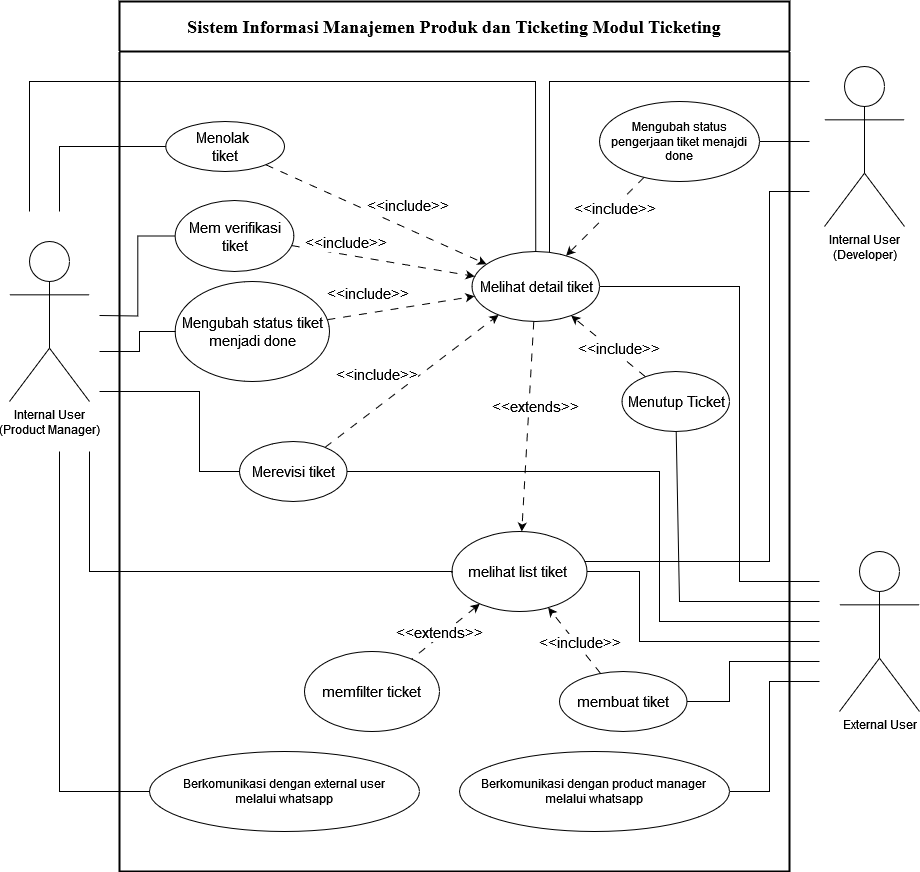
\includegraphics[width=0.8\textwidth]{images/use-case.png}
            \caption{Use Case Diagram Ticketing}
            \label{fig:use-case}
        \end{figure}
    \end{enumerate}

    \newpage

    \listsection{Analysis}

    \begin{enumerate} [label=\textbf{4.2.\arabic*.}, wide, labelwidth=!, labelindent=0pt]
        \listsection{Activity Diagram}

        Berdasarkan use case yang telah ditentukan, berikut adalah activity diagram untuk Sistem Informasi Manajemen Produk dan Ticketing bagian ticketing di PT. Teknologi Aplikasi Sejahtera

        \begin{enumerate}[label=\textbf{4.2.1.\arabic*.}, wide, labelwidth=!, labelindent=0pt]
            \listsection{Activity Diagram Internal User (Product Manager)}
            
            \begin{enumerate}[label=\arabic*.,wide,labelindent=27pt]
                \item Activity Diagram Melihat List Ticket
                
                \hspace*{10pt}
                \begin{tabularx}{.9\linewidth}{@{} l l X @{}}
                    ID Activity & : & AD-PM-01 \\
                    Deskripsi & : &  Activity Diagram berikut merupakan sebuah proses aktivitas yang dilakukan untuk melihat list ticket oleh seorang internal user dengan role product manager yang ditunjukkan pada gambar \ref{fig:AD-PM-01}.
                \end{tabularx}
                

                \begin{figure}[H]
                    \centering 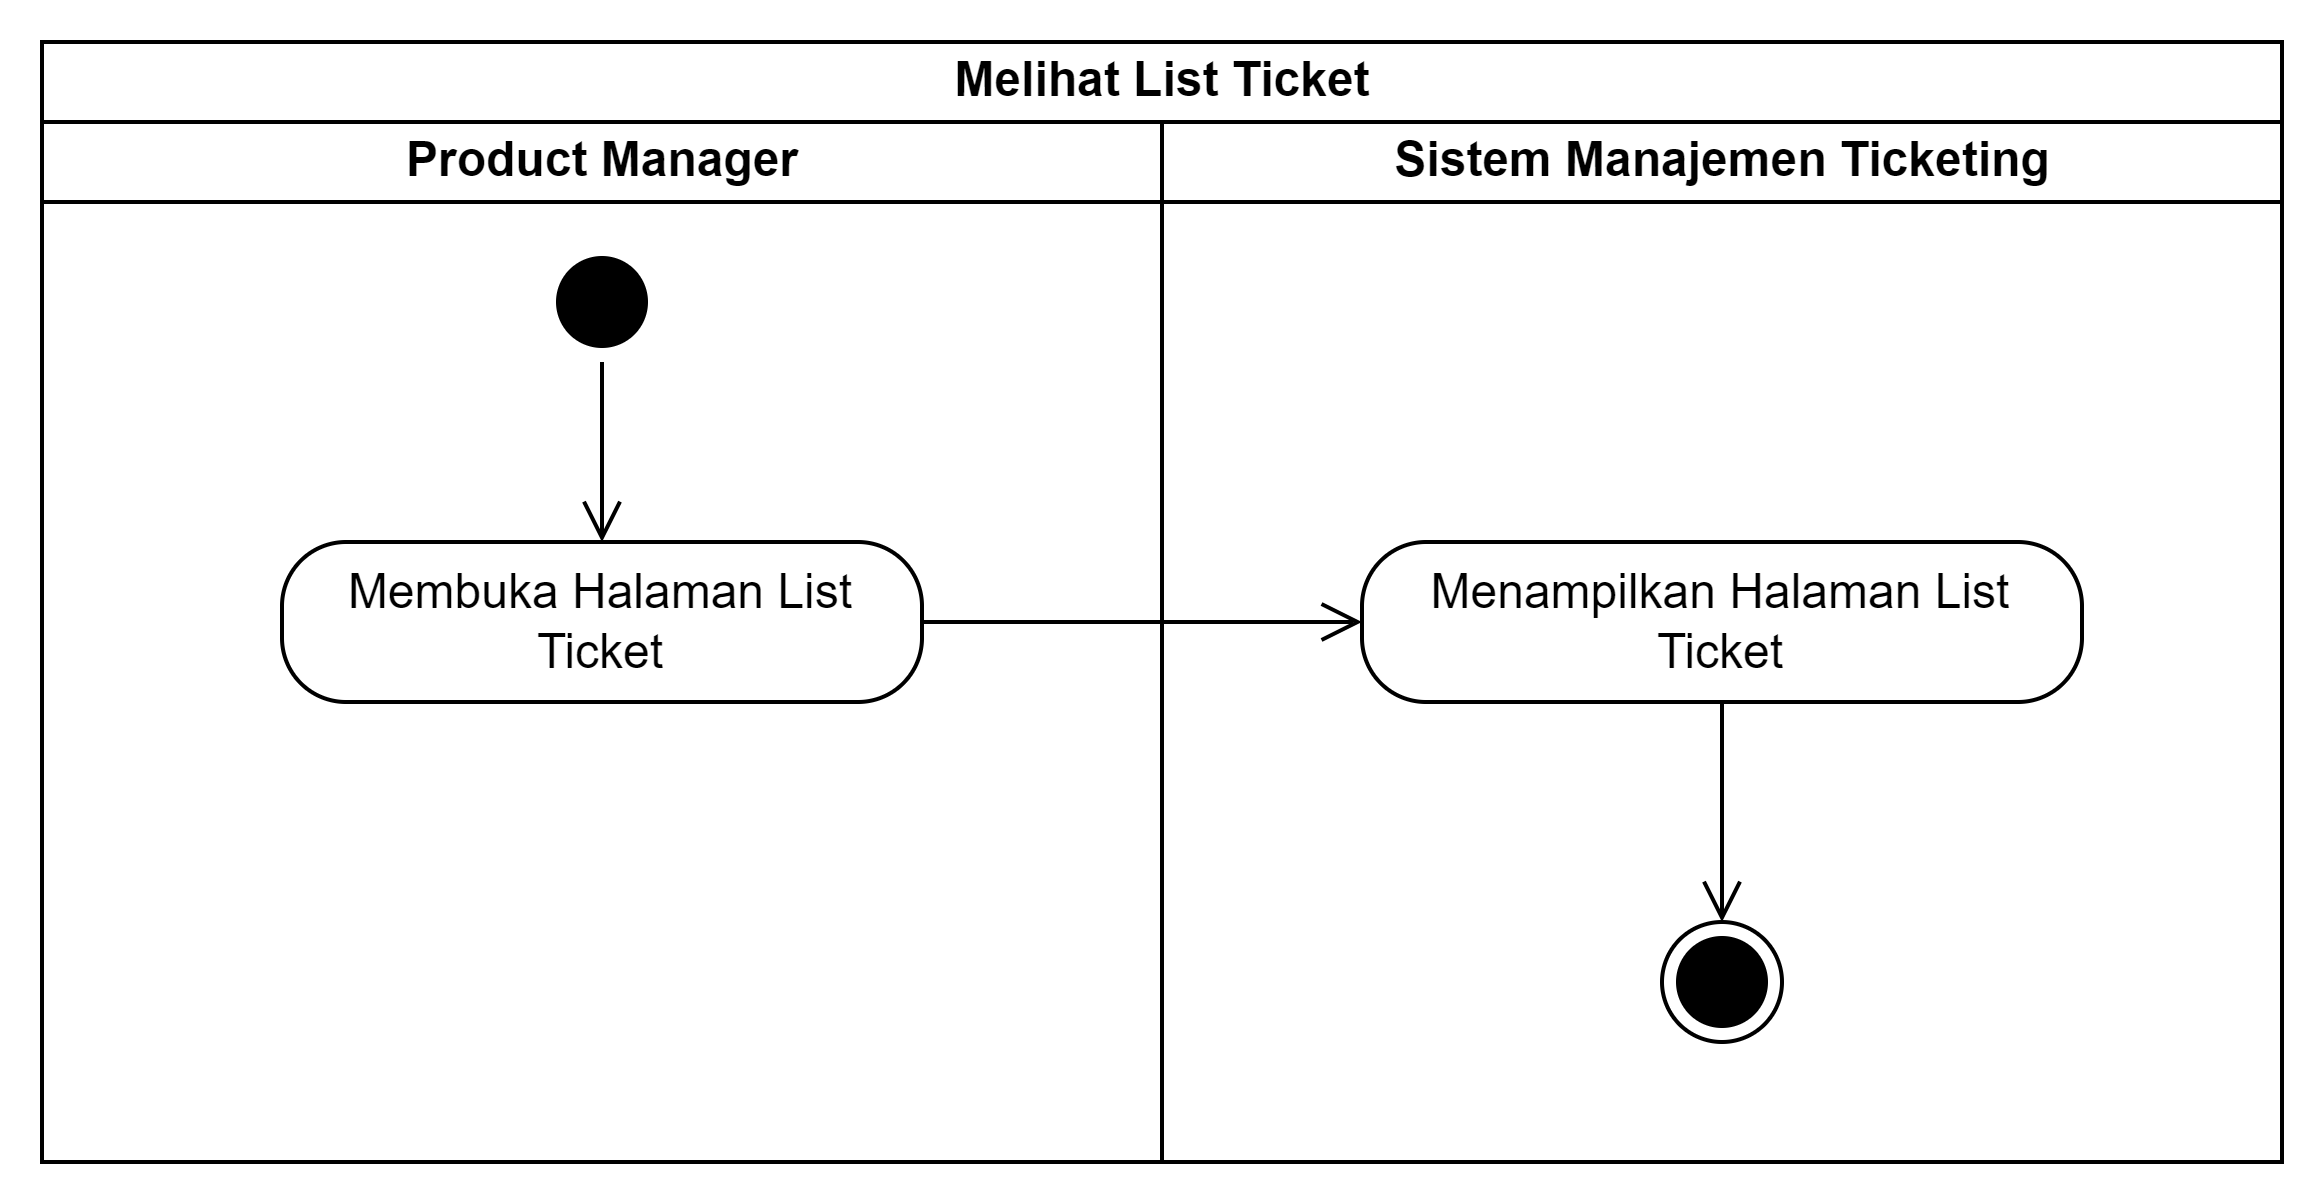
\includegraphics[width=0.75\textwidth]{images/activity/ipm/Melihat List Ticket.png}
                    \caption{Activity Diagram Melihat List Ticket (PM)}
                    \label{fig:AD-PM-01}
                \end{figure}

                \item Activity Diagram Memfilter Ticket
                
                \hspace*{10pt}
                \begin{tabularx}{.9\linewidth}{@{} l l X @{}}
                    ID Activity & : & AD-PM-02 \\
                    Deskripsi & : &  Activity Diagram berikut merupakan sebuah proses aktivitas yang dilakukan untuk memfilter ticket oleh seorang internal user dengan role product manager yang ditunjukkan pada gambar \ref{fig:AD-PM-02}
                \end{tabularx}
                
                \begin{figure}[H]
                    \centering 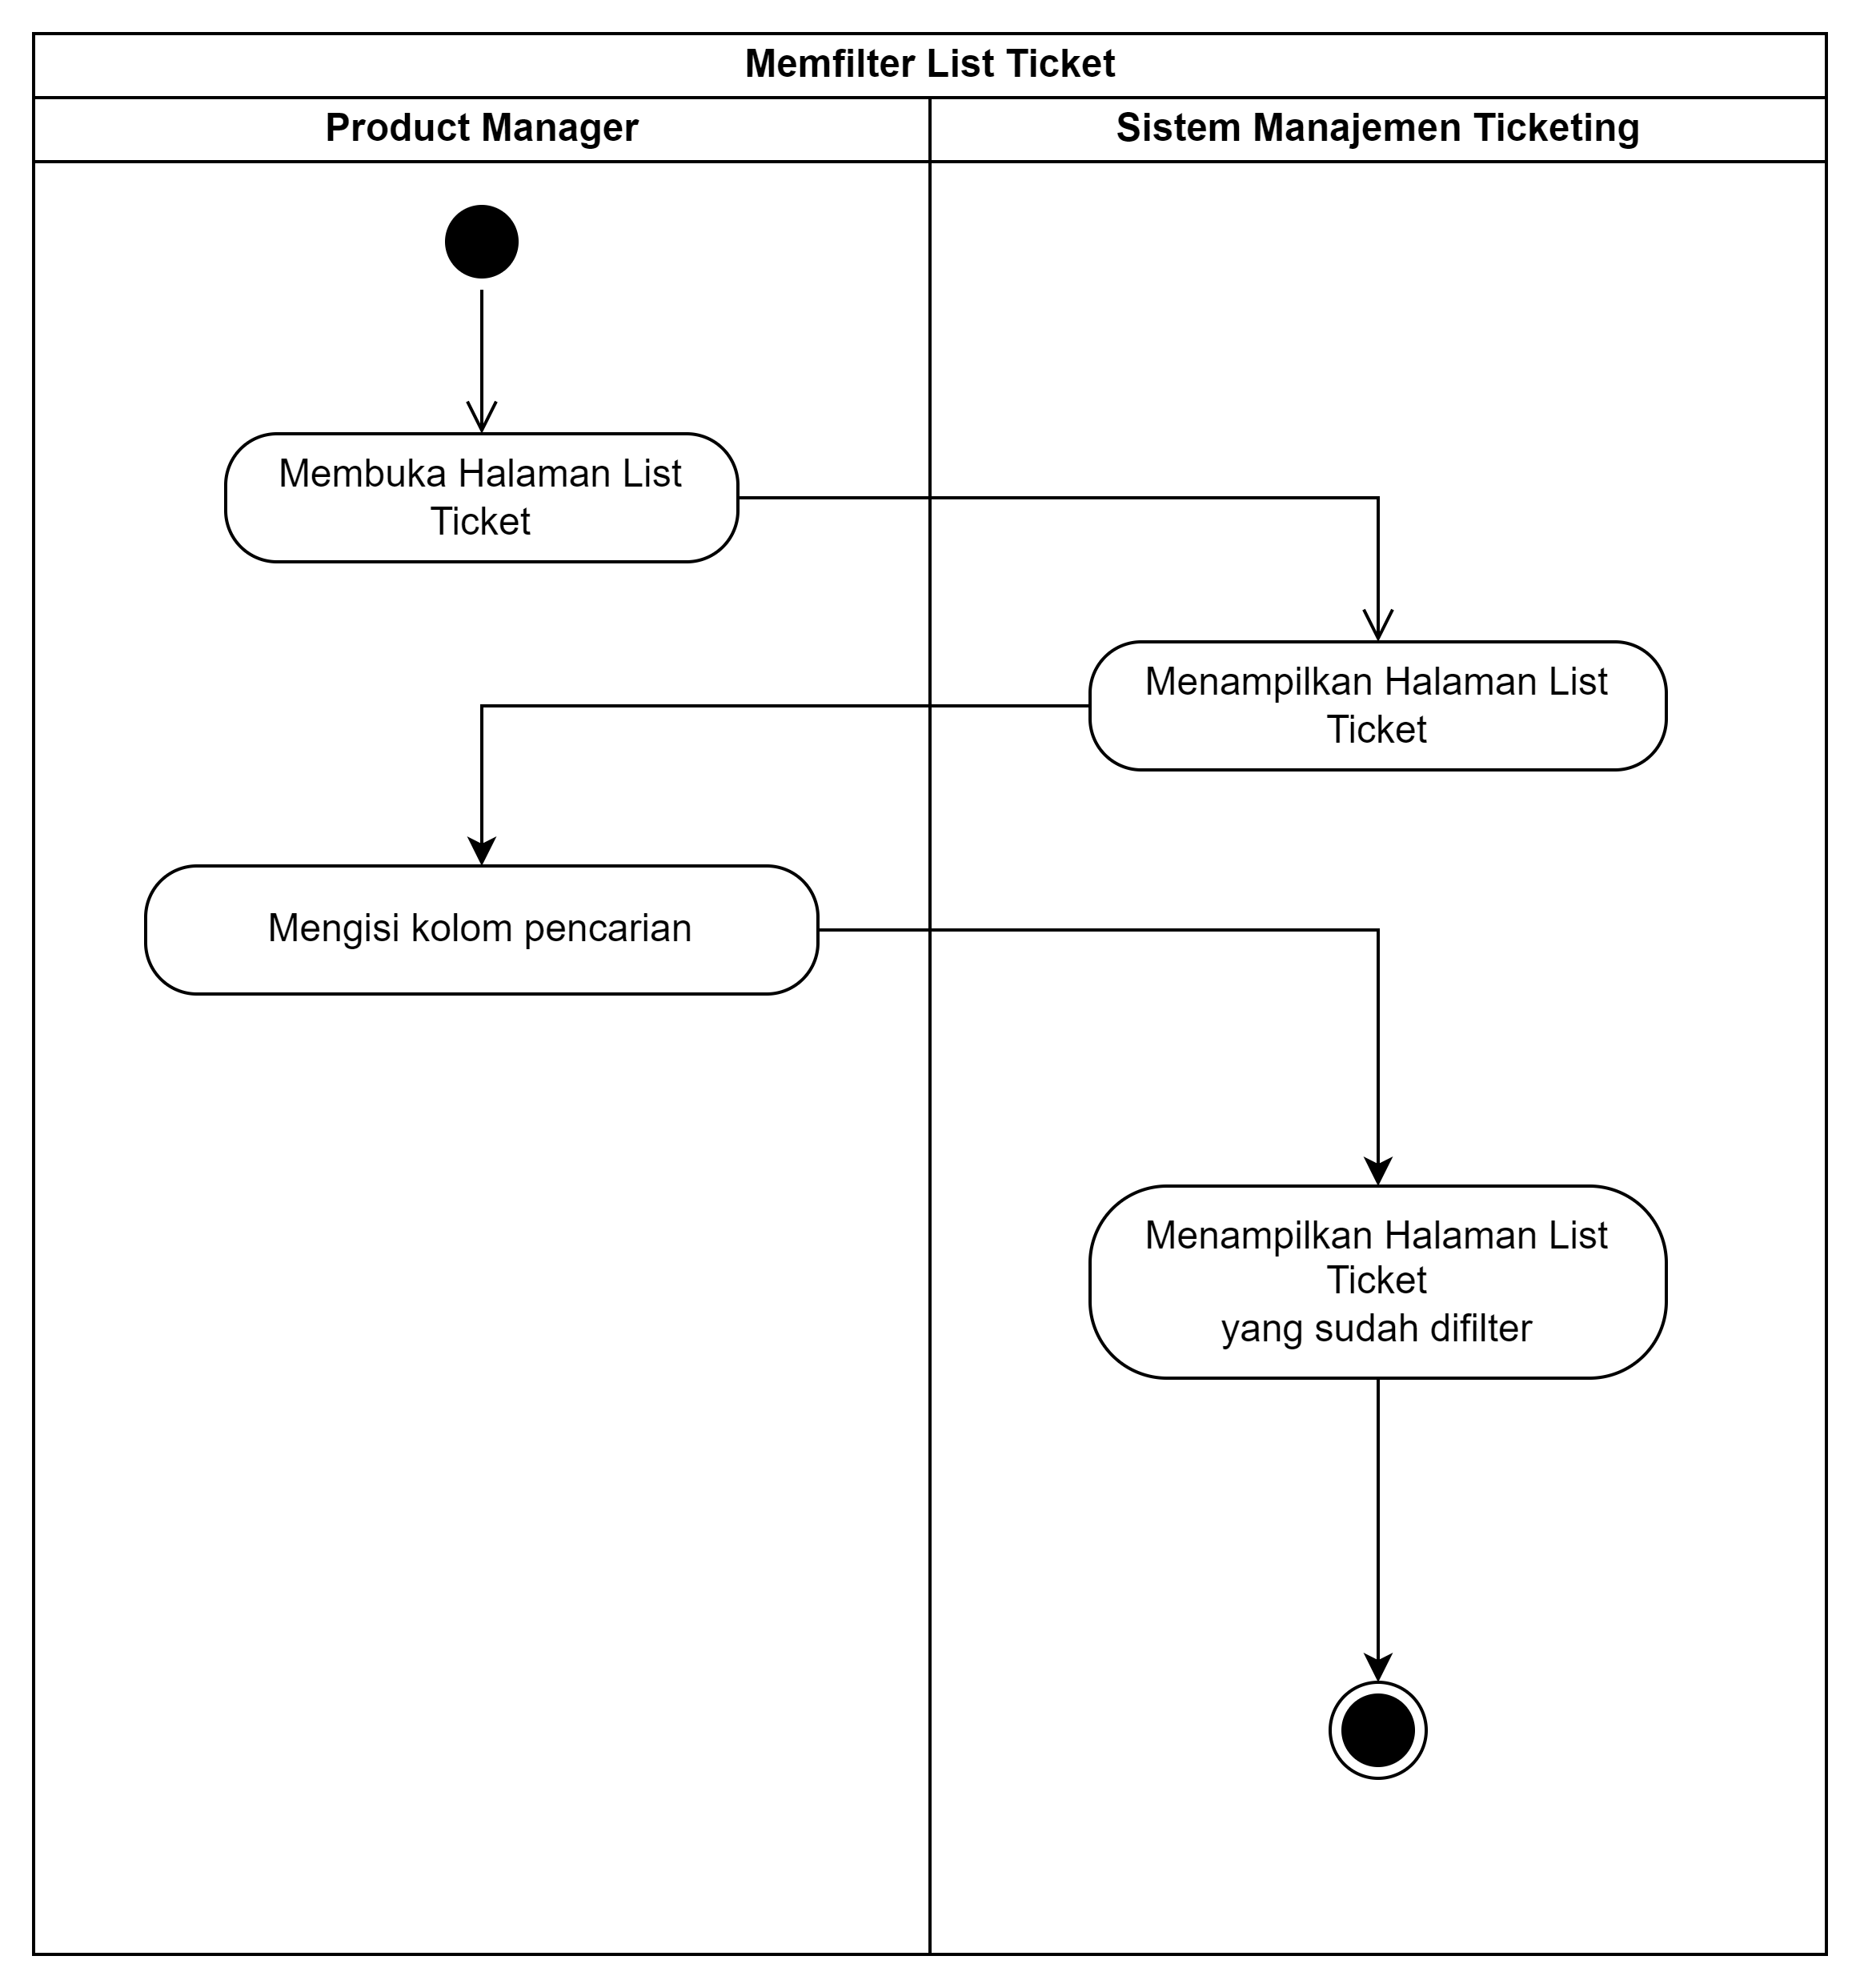
\includegraphics[width=0.75\textwidth]{images/activity/ipm/Memfilter List Ticket.png}
                    \caption{Activity Diagram Memfilter List Ticket (PM)}
                    \label{fig:AD-PM-02}
                \end{figure}

                \item Activity Diagram Melihat Detail Ticket
                
                \hspace*{10pt}
                \begin{tabularx}{.9\linewidth}{@{} l l X @{}}
                    ID Activity & : & AD-PM-03 \\

                    Deskripsi &	: & Activity Diagram berikut merupakan sebuah proses aktivitas yang dilakukan untuk melihat detail ticket oleh seorang  internal user dengan role product manager yang ditunjukkan pada gambar 4.4.
                \end{tabularx}

                \begin{figure}[H]
                    \centering 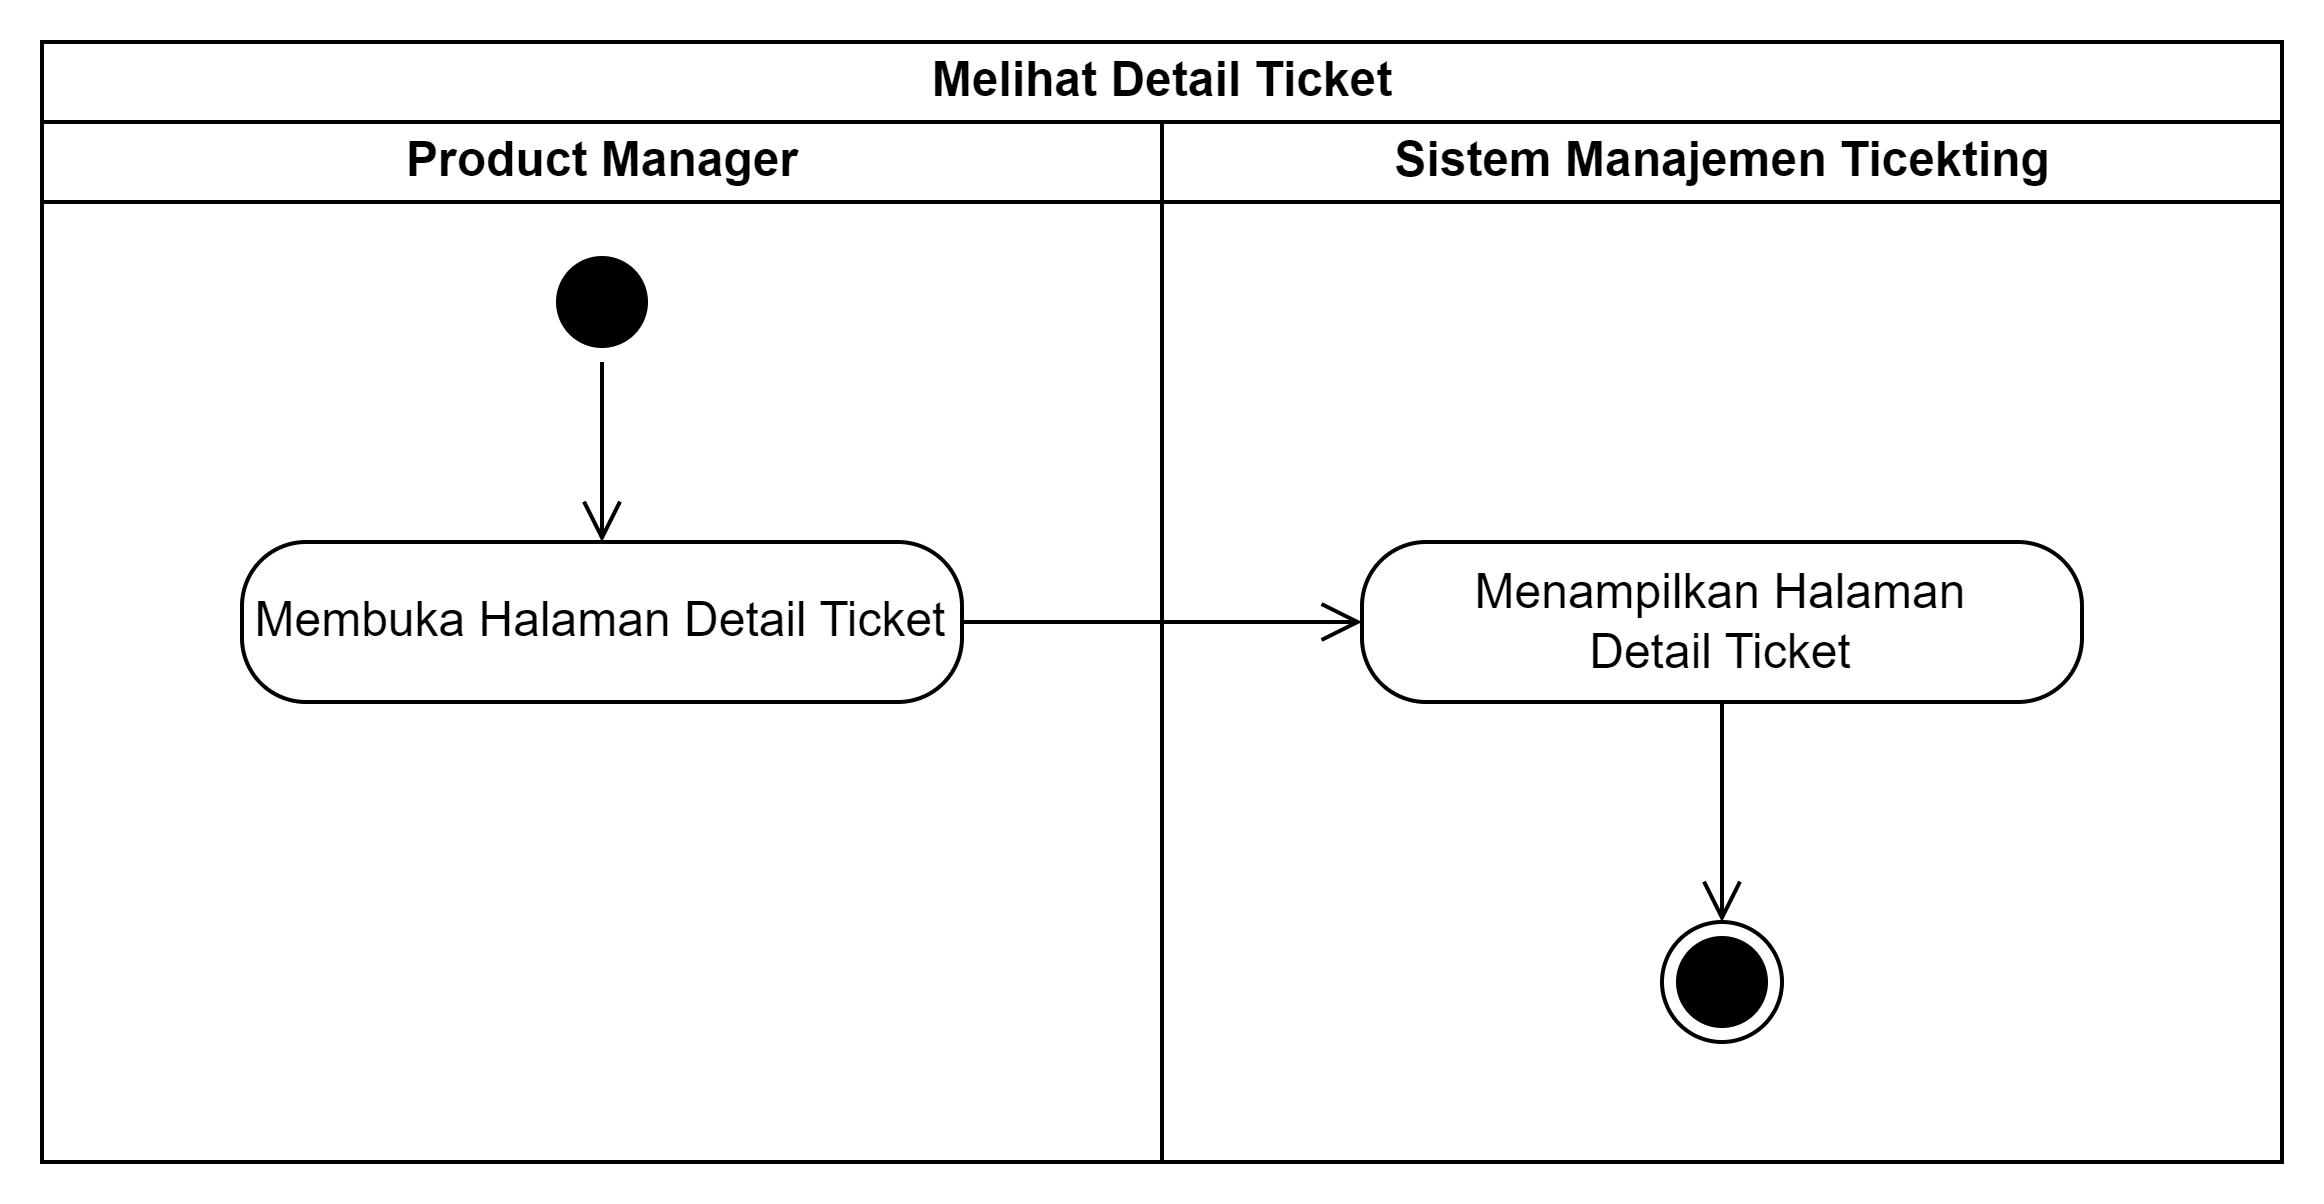
\includegraphics[width=0.75\textwidth]{images/activity/ipm/Melihat Detail Ticket.png}
                    \caption{Activity Diagram Melihat Detail Ticket (PM)}
                    \label{fig:AD-PM-03}
                \end{figure}

                \item Activity Diagram Memverifikasi Ticket

                \hspace*{10pt}
                \begin{tabularx}{.9\linewidth}{@{} l l X @{}}
                    ID Activity & : & AD-PM-04 \\

                    Deskripsi &	: & Activity Diagram berikut merupakan sebuah proses aktivitas yang dilakukan untuk memverifikasi ticket yang dibuat external user oleh seorang  internal user dengan role product manager yang ditunjukkan pada gambar 4.5.
                \end{tabularx}

                \begin{figure}[H]
                    \centering 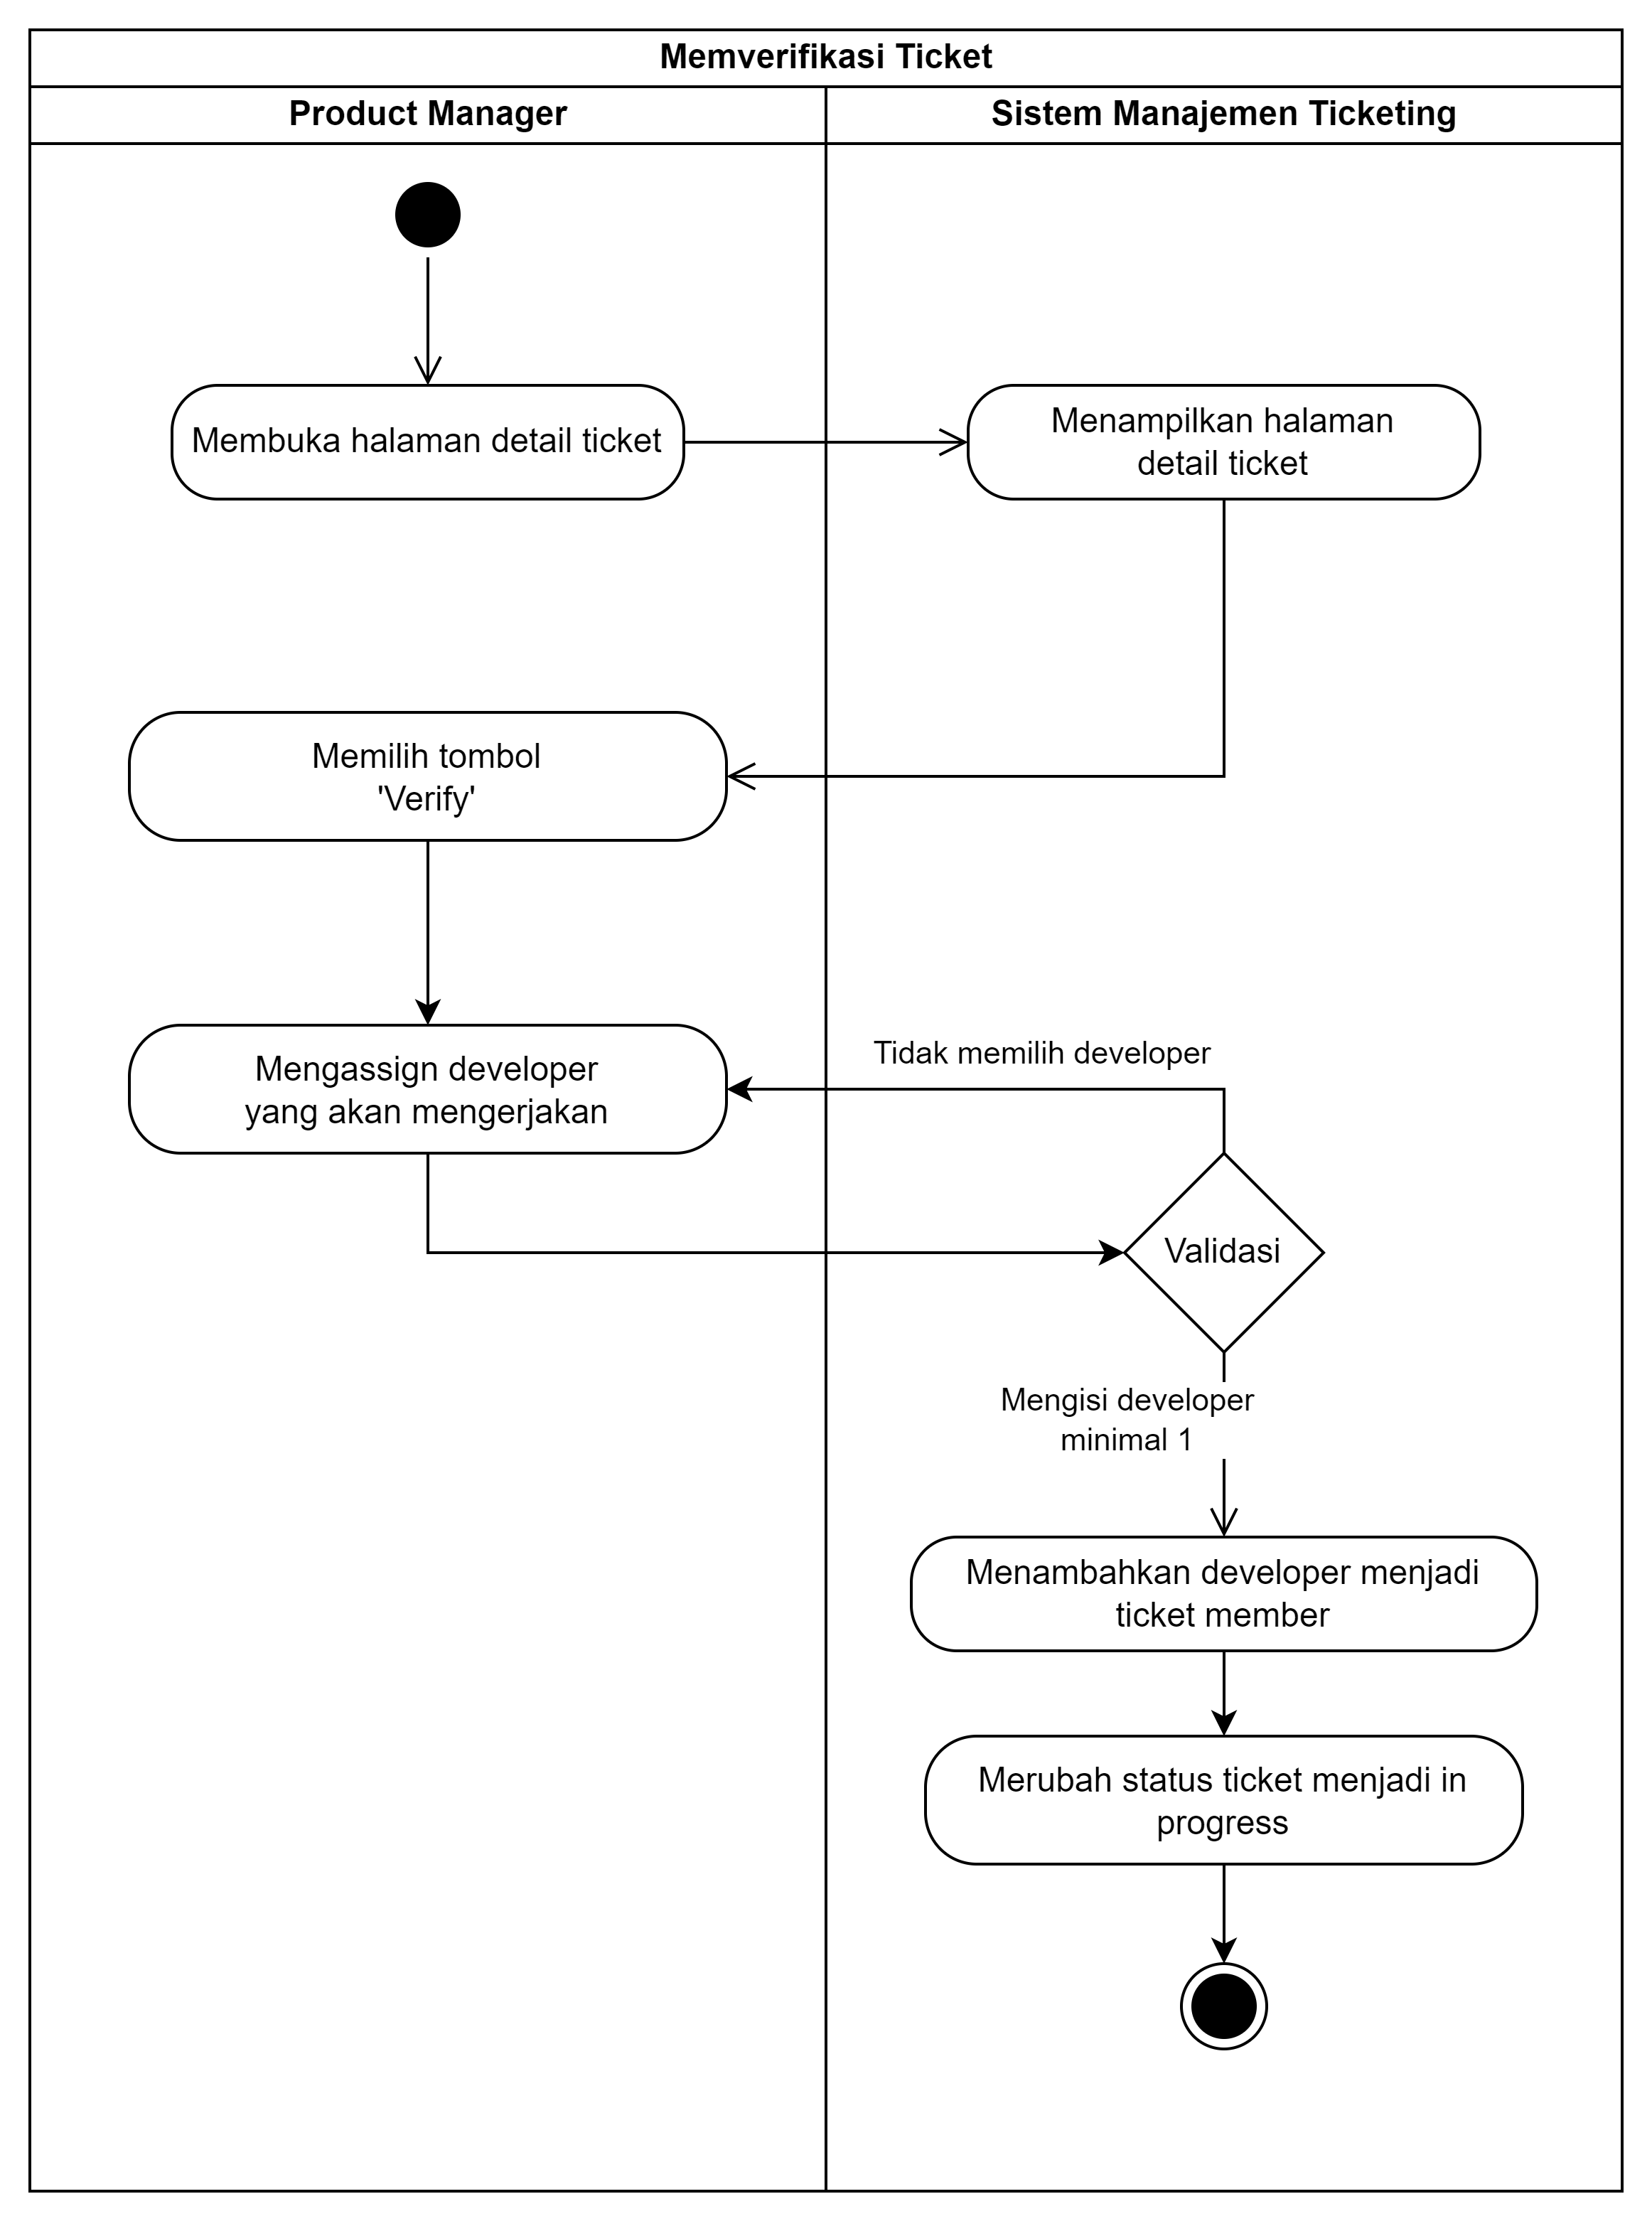
\includegraphics[width=0.75\textwidth]{images/activity/ipm/Memverifikasi Ticket.png}
                    \caption{Activity Diagram Memverifikasi Ticket (PM)}
                    \label{fig:AD-PM-04}
                \end{figure}


                \item Activity Diagram Menolak Ticket

                \hspace*{10pt}
                \begin{tabularx}{.9\linewidth}{@{} l l X @{}}
                    ID Activity & : & AD-PM-05 \\

                    Deskripsi &	: & Activity Diagram berikut merupakan sebuah proses aktivitas yang dilakukan untuk menolak ticket yang dibuat external user oleh seorang  internal user dengan role product manager yang ditunjukkan pada gambar 4.6.
                \end{tabularx}

                \begin{figure}[H]
                    \centering 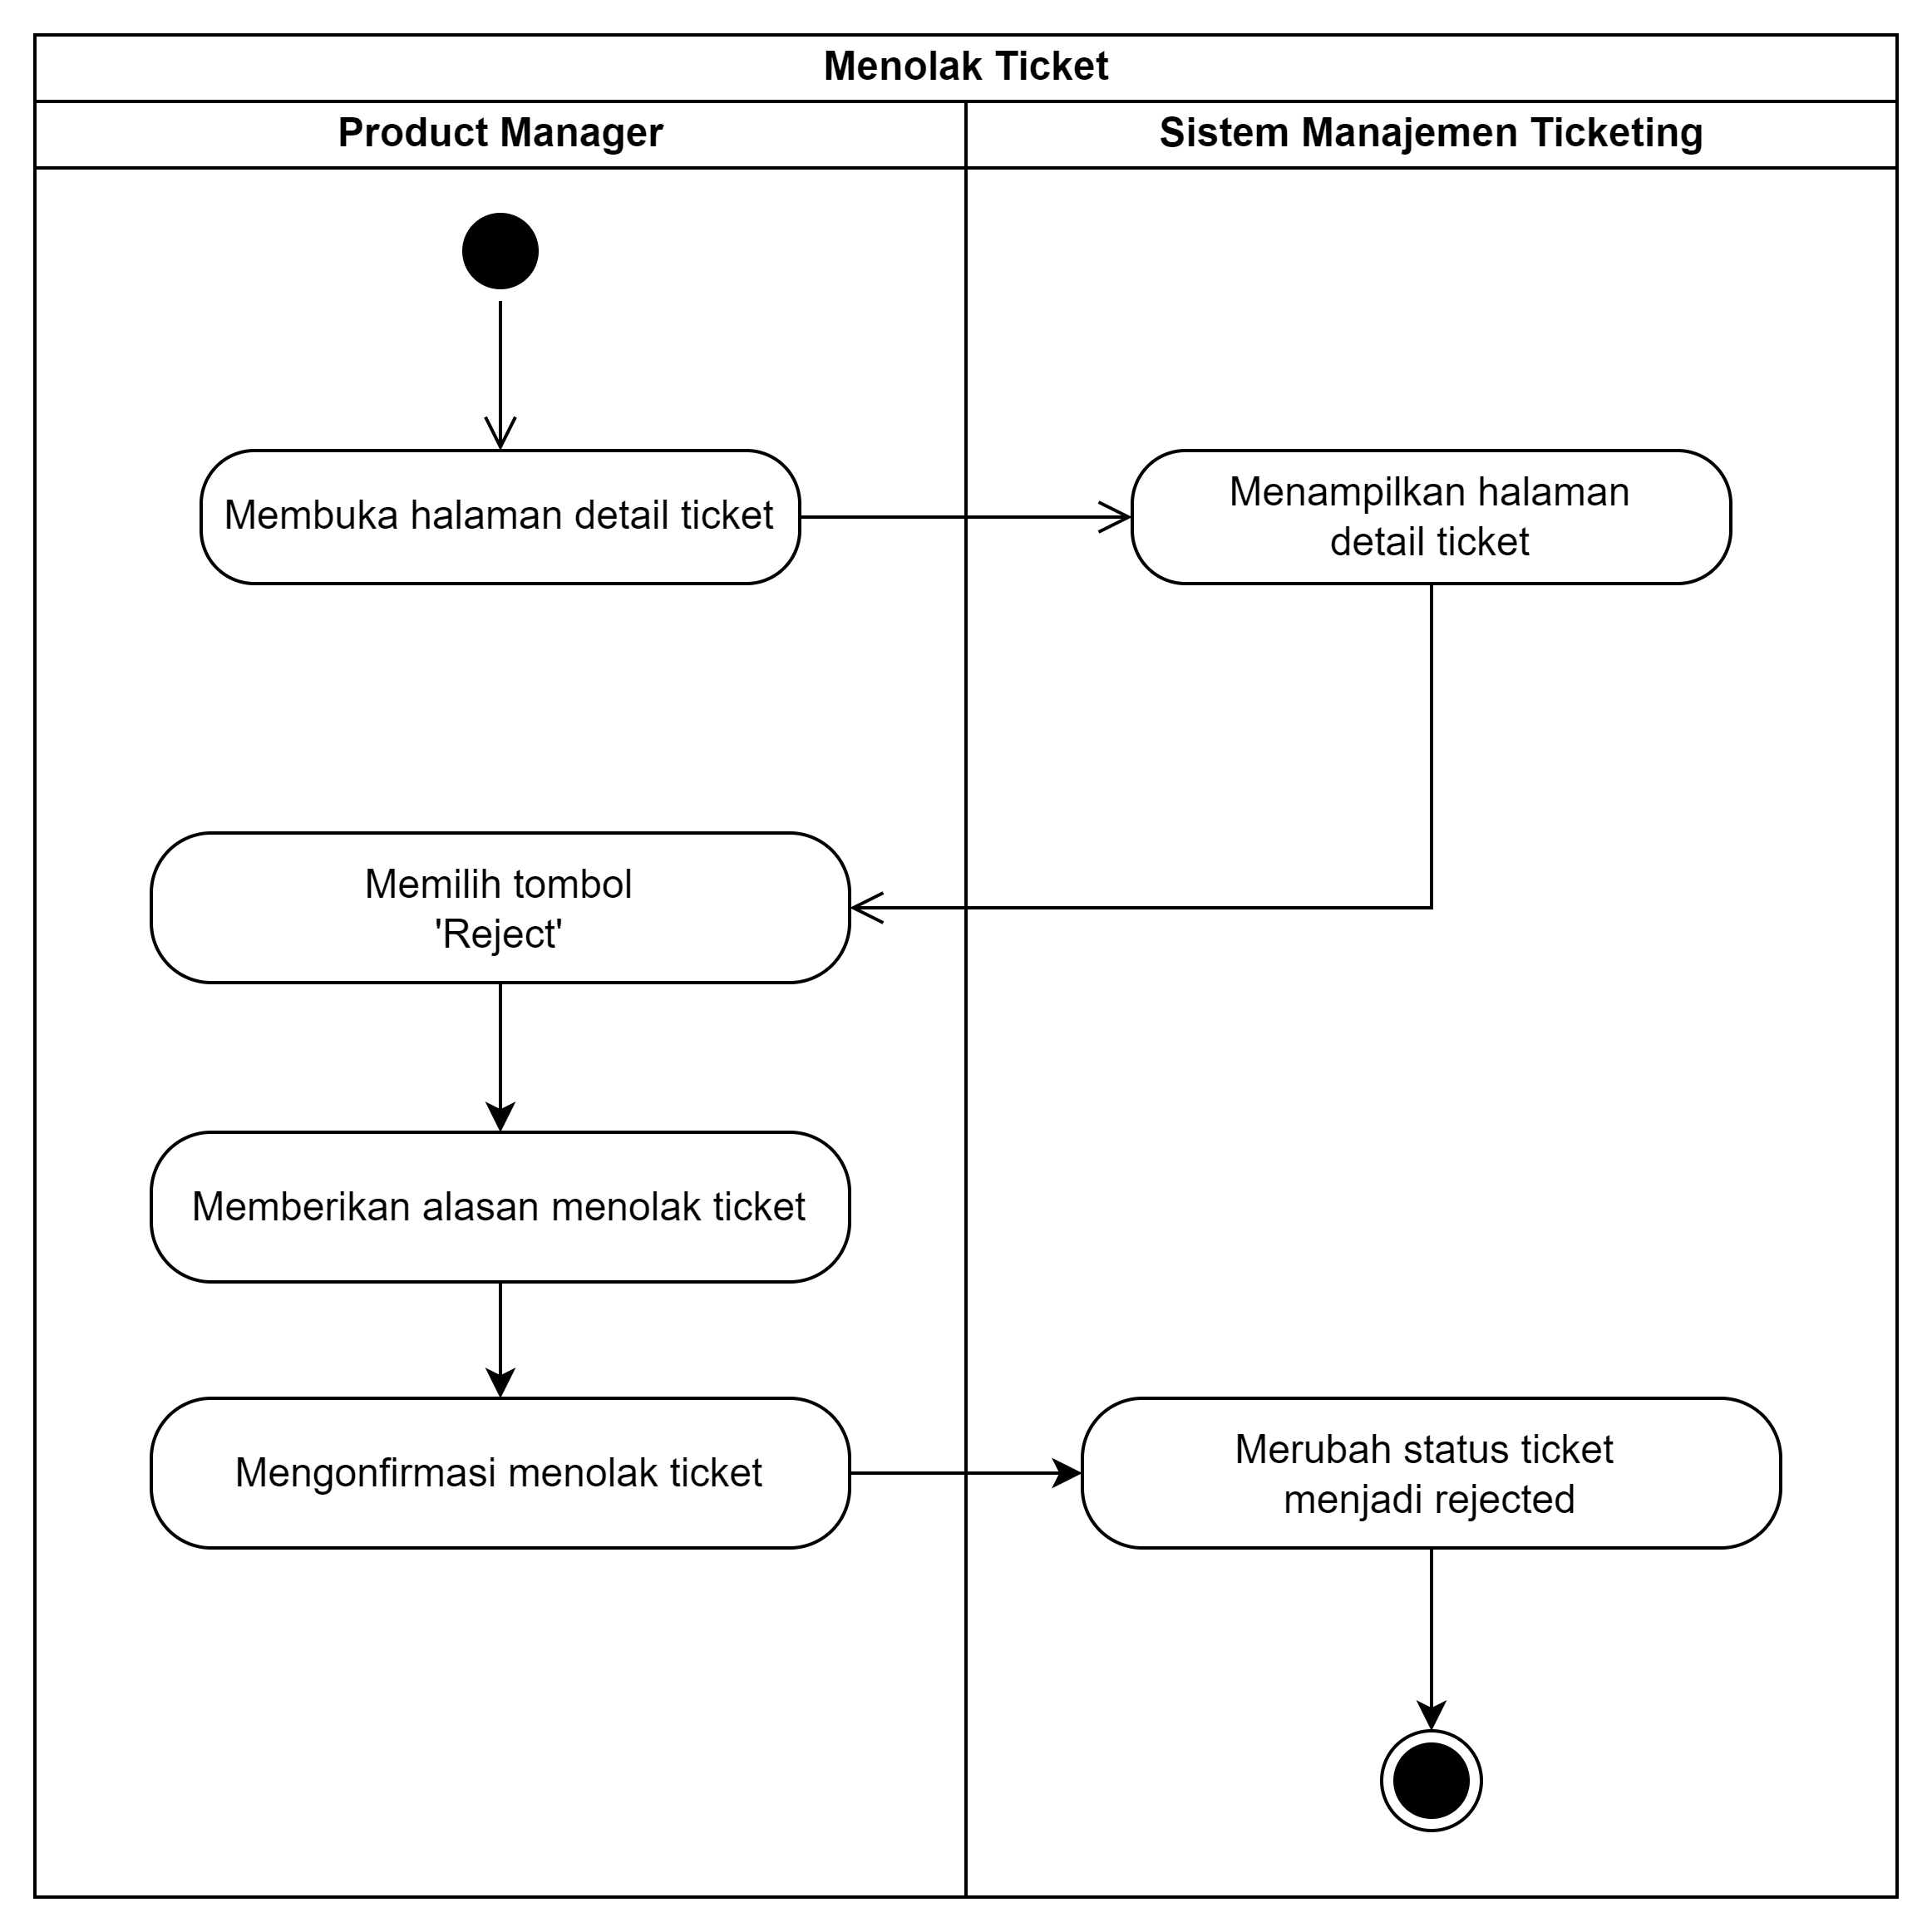
\includegraphics[width=0.75\textwidth]{images/activity/ipm/Menolak Ticket.png}
                    \caption{Activity Diagram Menolak Ticket (PM)}
                    \label{fig:AD-PM-05}
                \end{figure}

                \item Activity Diagram Merevisi Ticket

                \hspace*{10pt}
                \begin{tabularx}{.9\linewidth}{@{} l l X @{}}
                    ID Activity & : & AD-PM-06 \\

                    Deskripsi &	: & Activity Diagram berikut merupakan sebuah proses aktivitas yang dilakukan untuk merevisi ticket yang telah dikerjakan developer oleh seorang  internal user dengan role product manager yang ditunjukkan pada gambar 4.7.
                \end{tabularx}

                \begin{figure}[H]
                    \centering 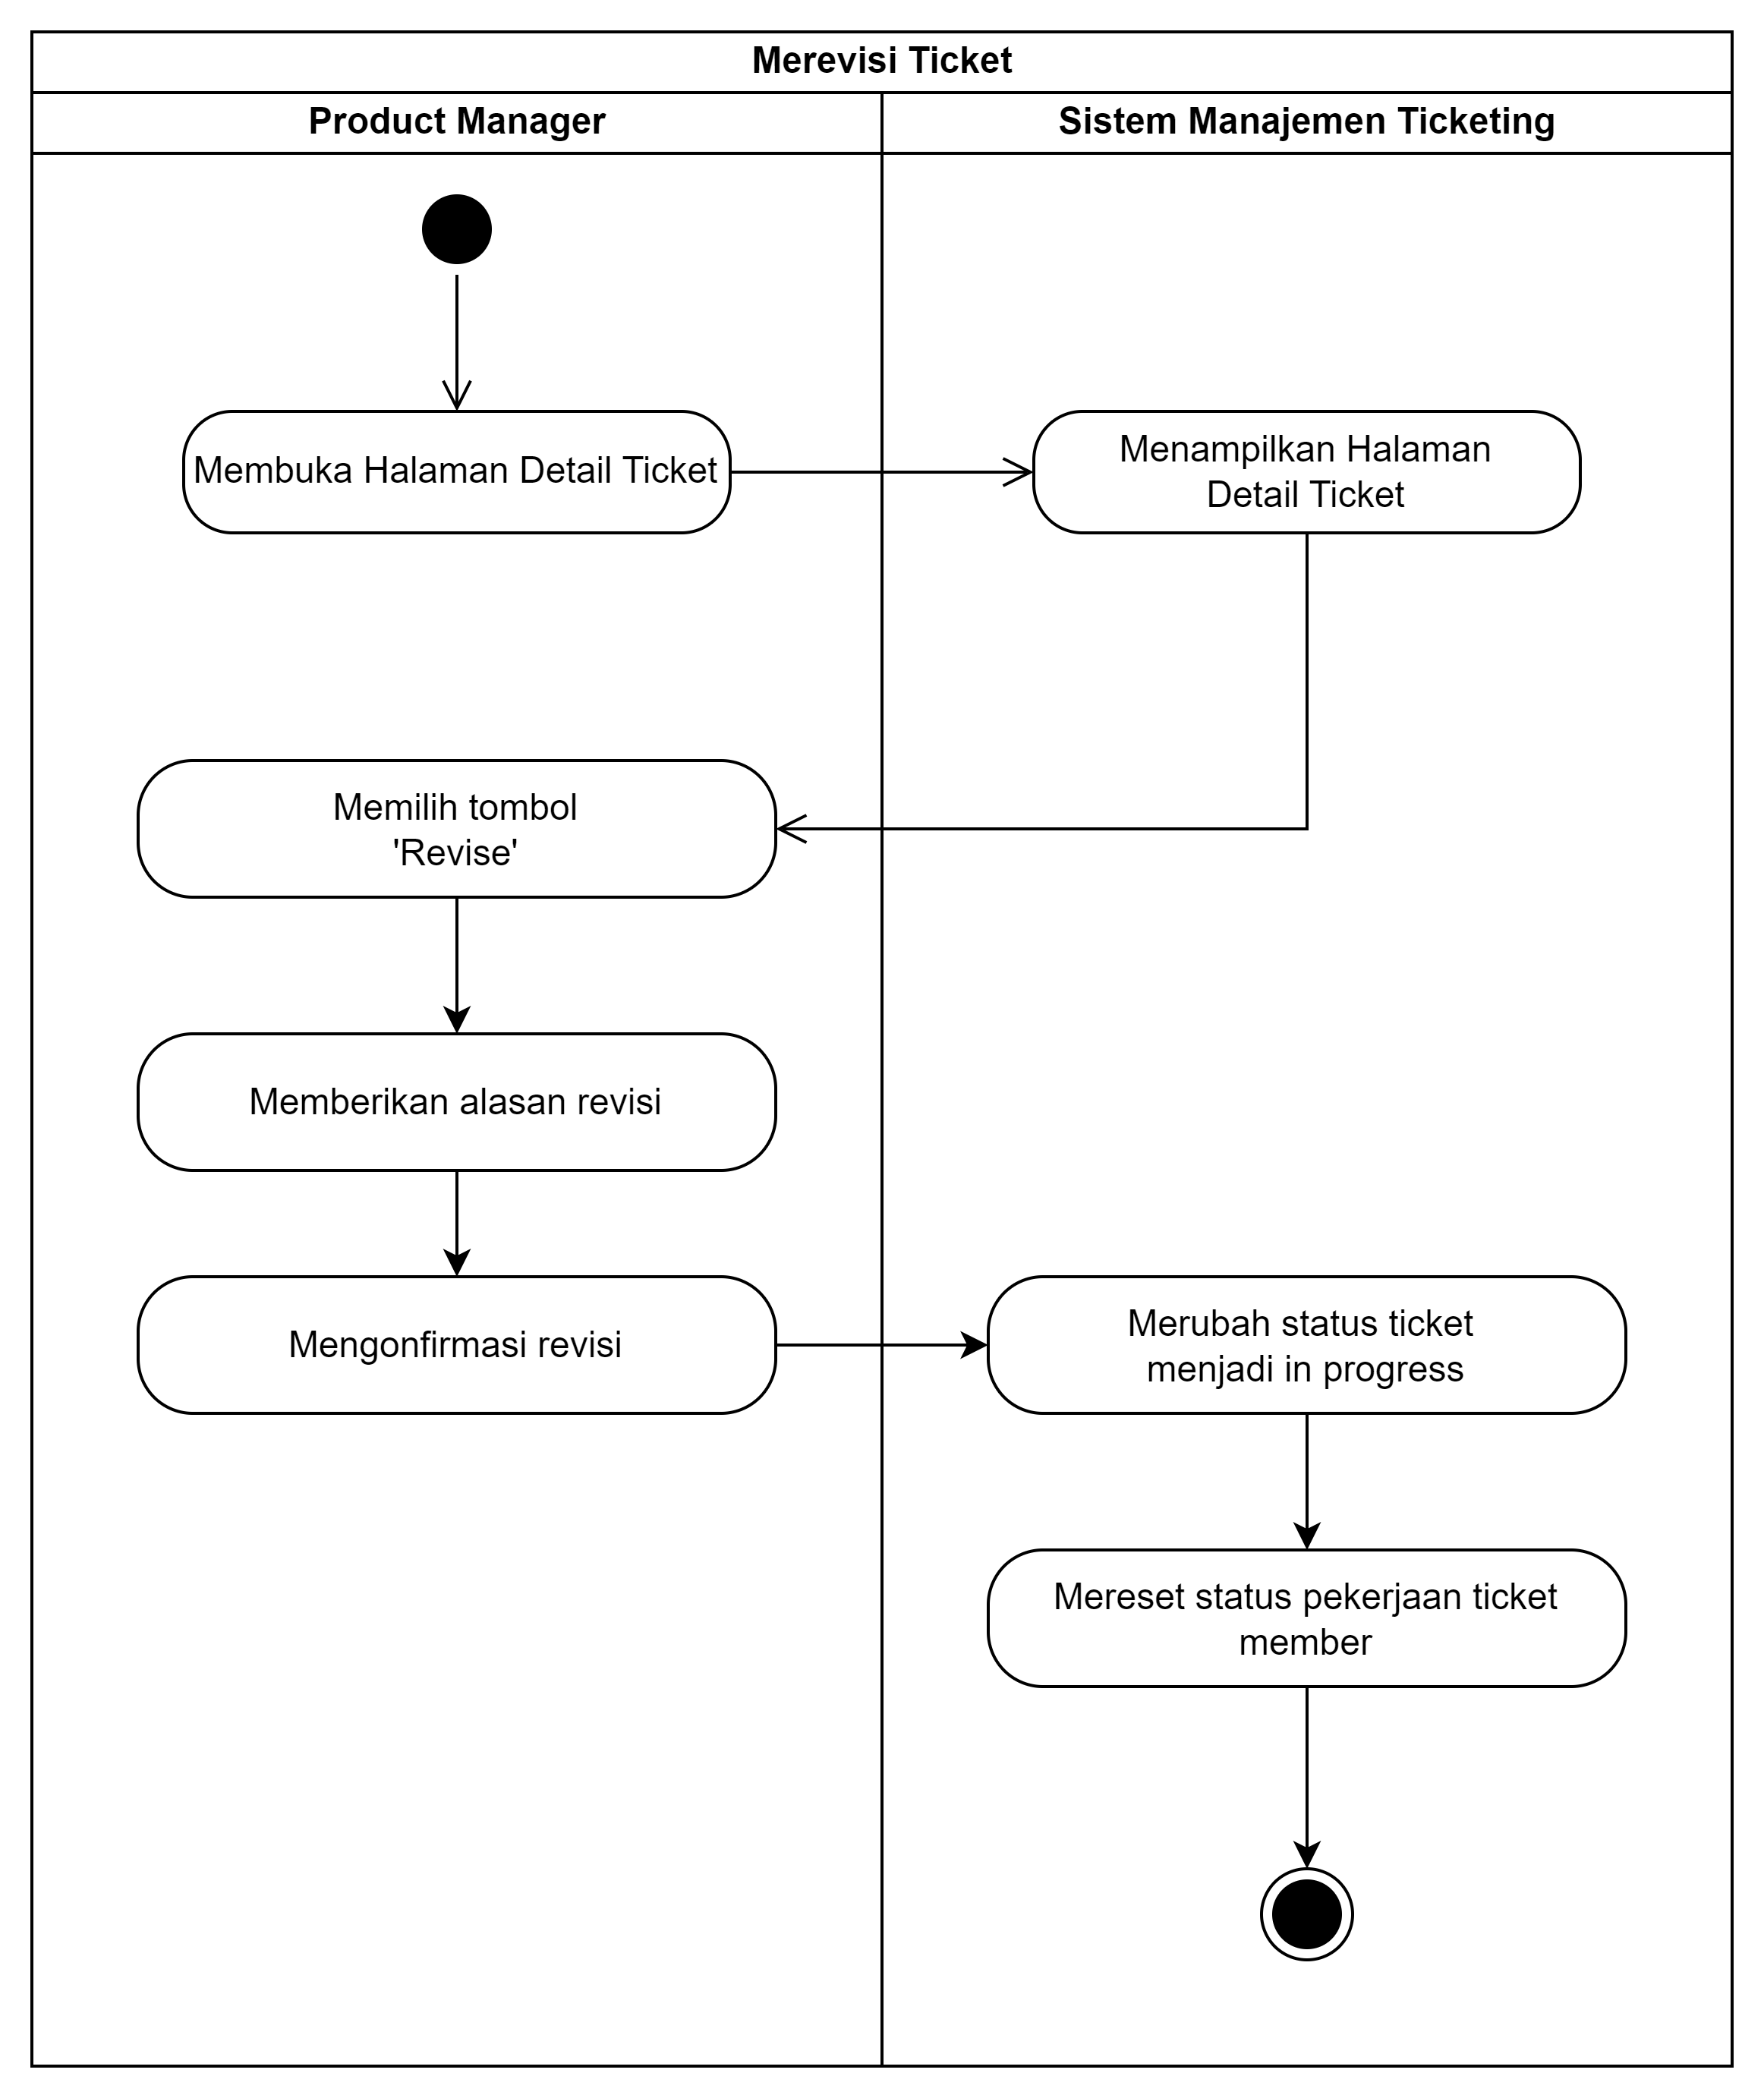
\includegraphics[width=0.75\textwidth]{images/activity/ipm/Merevisi Ticket.png}
                    \caption{Activity Diagram Merevisi Ticket (PM)}
                    \label{fig:AD-PM-06}
                \end{figure}

                \item Activity Diagram Berkomunikasi dengan external user

                \hspace*{10pt}
                \begin{tabularx}{.9\linewidth}{@{} l l X @{}}
                    ID Activity & : & AD-PM-07 \\

                    Deskripsi &	: & Activity Diagram berikut merupakan sebuah proses aktivitas yang dilakukan untuk berkomunikasi dengan external user oleh seorang  internal user dengan role product manager yang ditunjukkan pada gambar 4.8.
                \end{tabularx}

                \begin{figure}[H]
                    \centering 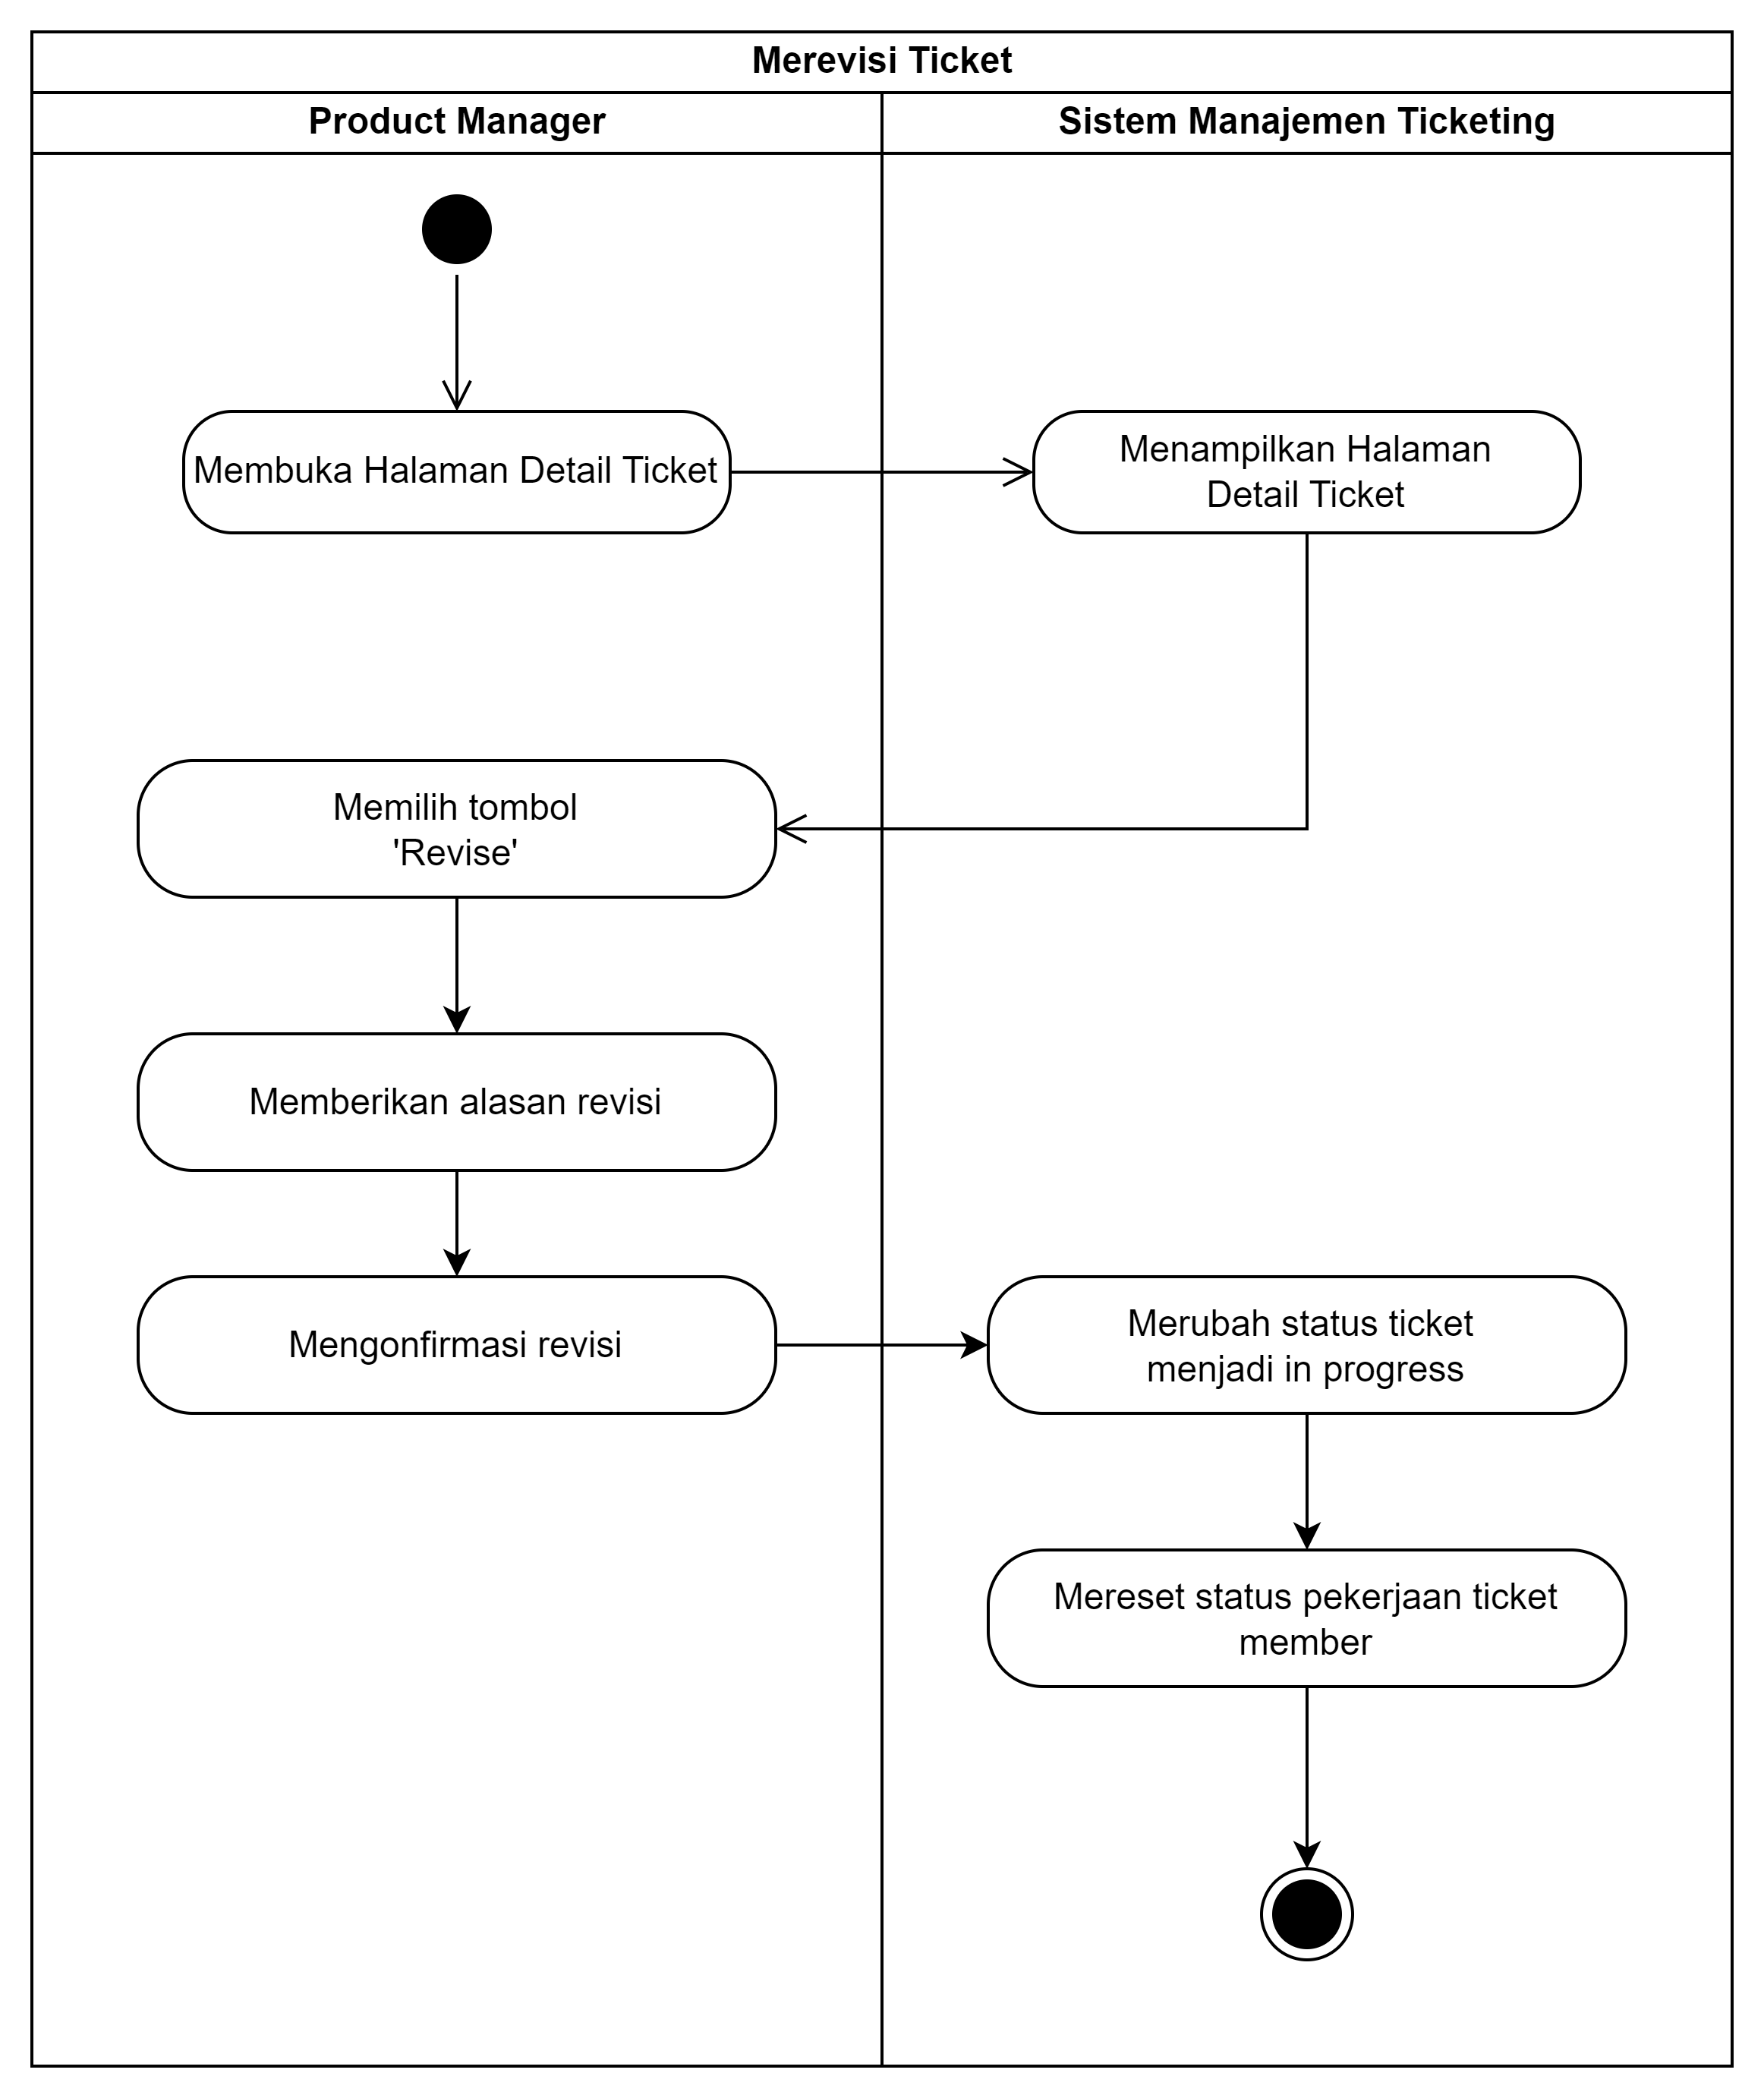
\includegraphics[width=0.75\textwidth]{images/activity/ipm/Berkomunikasi Dengan External User Melalui Whatsapp.png}
                    \caption{Activity Diagram Berkomunikasi Dengan PM Melalui Whatsapp (PM)}
                    \label{fig:AD-PM-07}
                \end{figure}

                \item Activity Diagram Mengubah Status Ticket Menjadi Done

                \hspace*{10pt}
                \begin{tabularx}{.9\linewidth}{@{} l l X @{}}
                    ID Activity & : & AD-PM-08 \\

                    Deskripsi &	: & Activity Diagram berikut merupakan sebuah proses aktivitas yang dilakukan untuk mengubah status ticket menjadi done oleh internal user dengan role product manager yang ditunjukkan pada gambar 4.9.
                \end{tabularx}

                \begin{figure}[H]
                    \centering 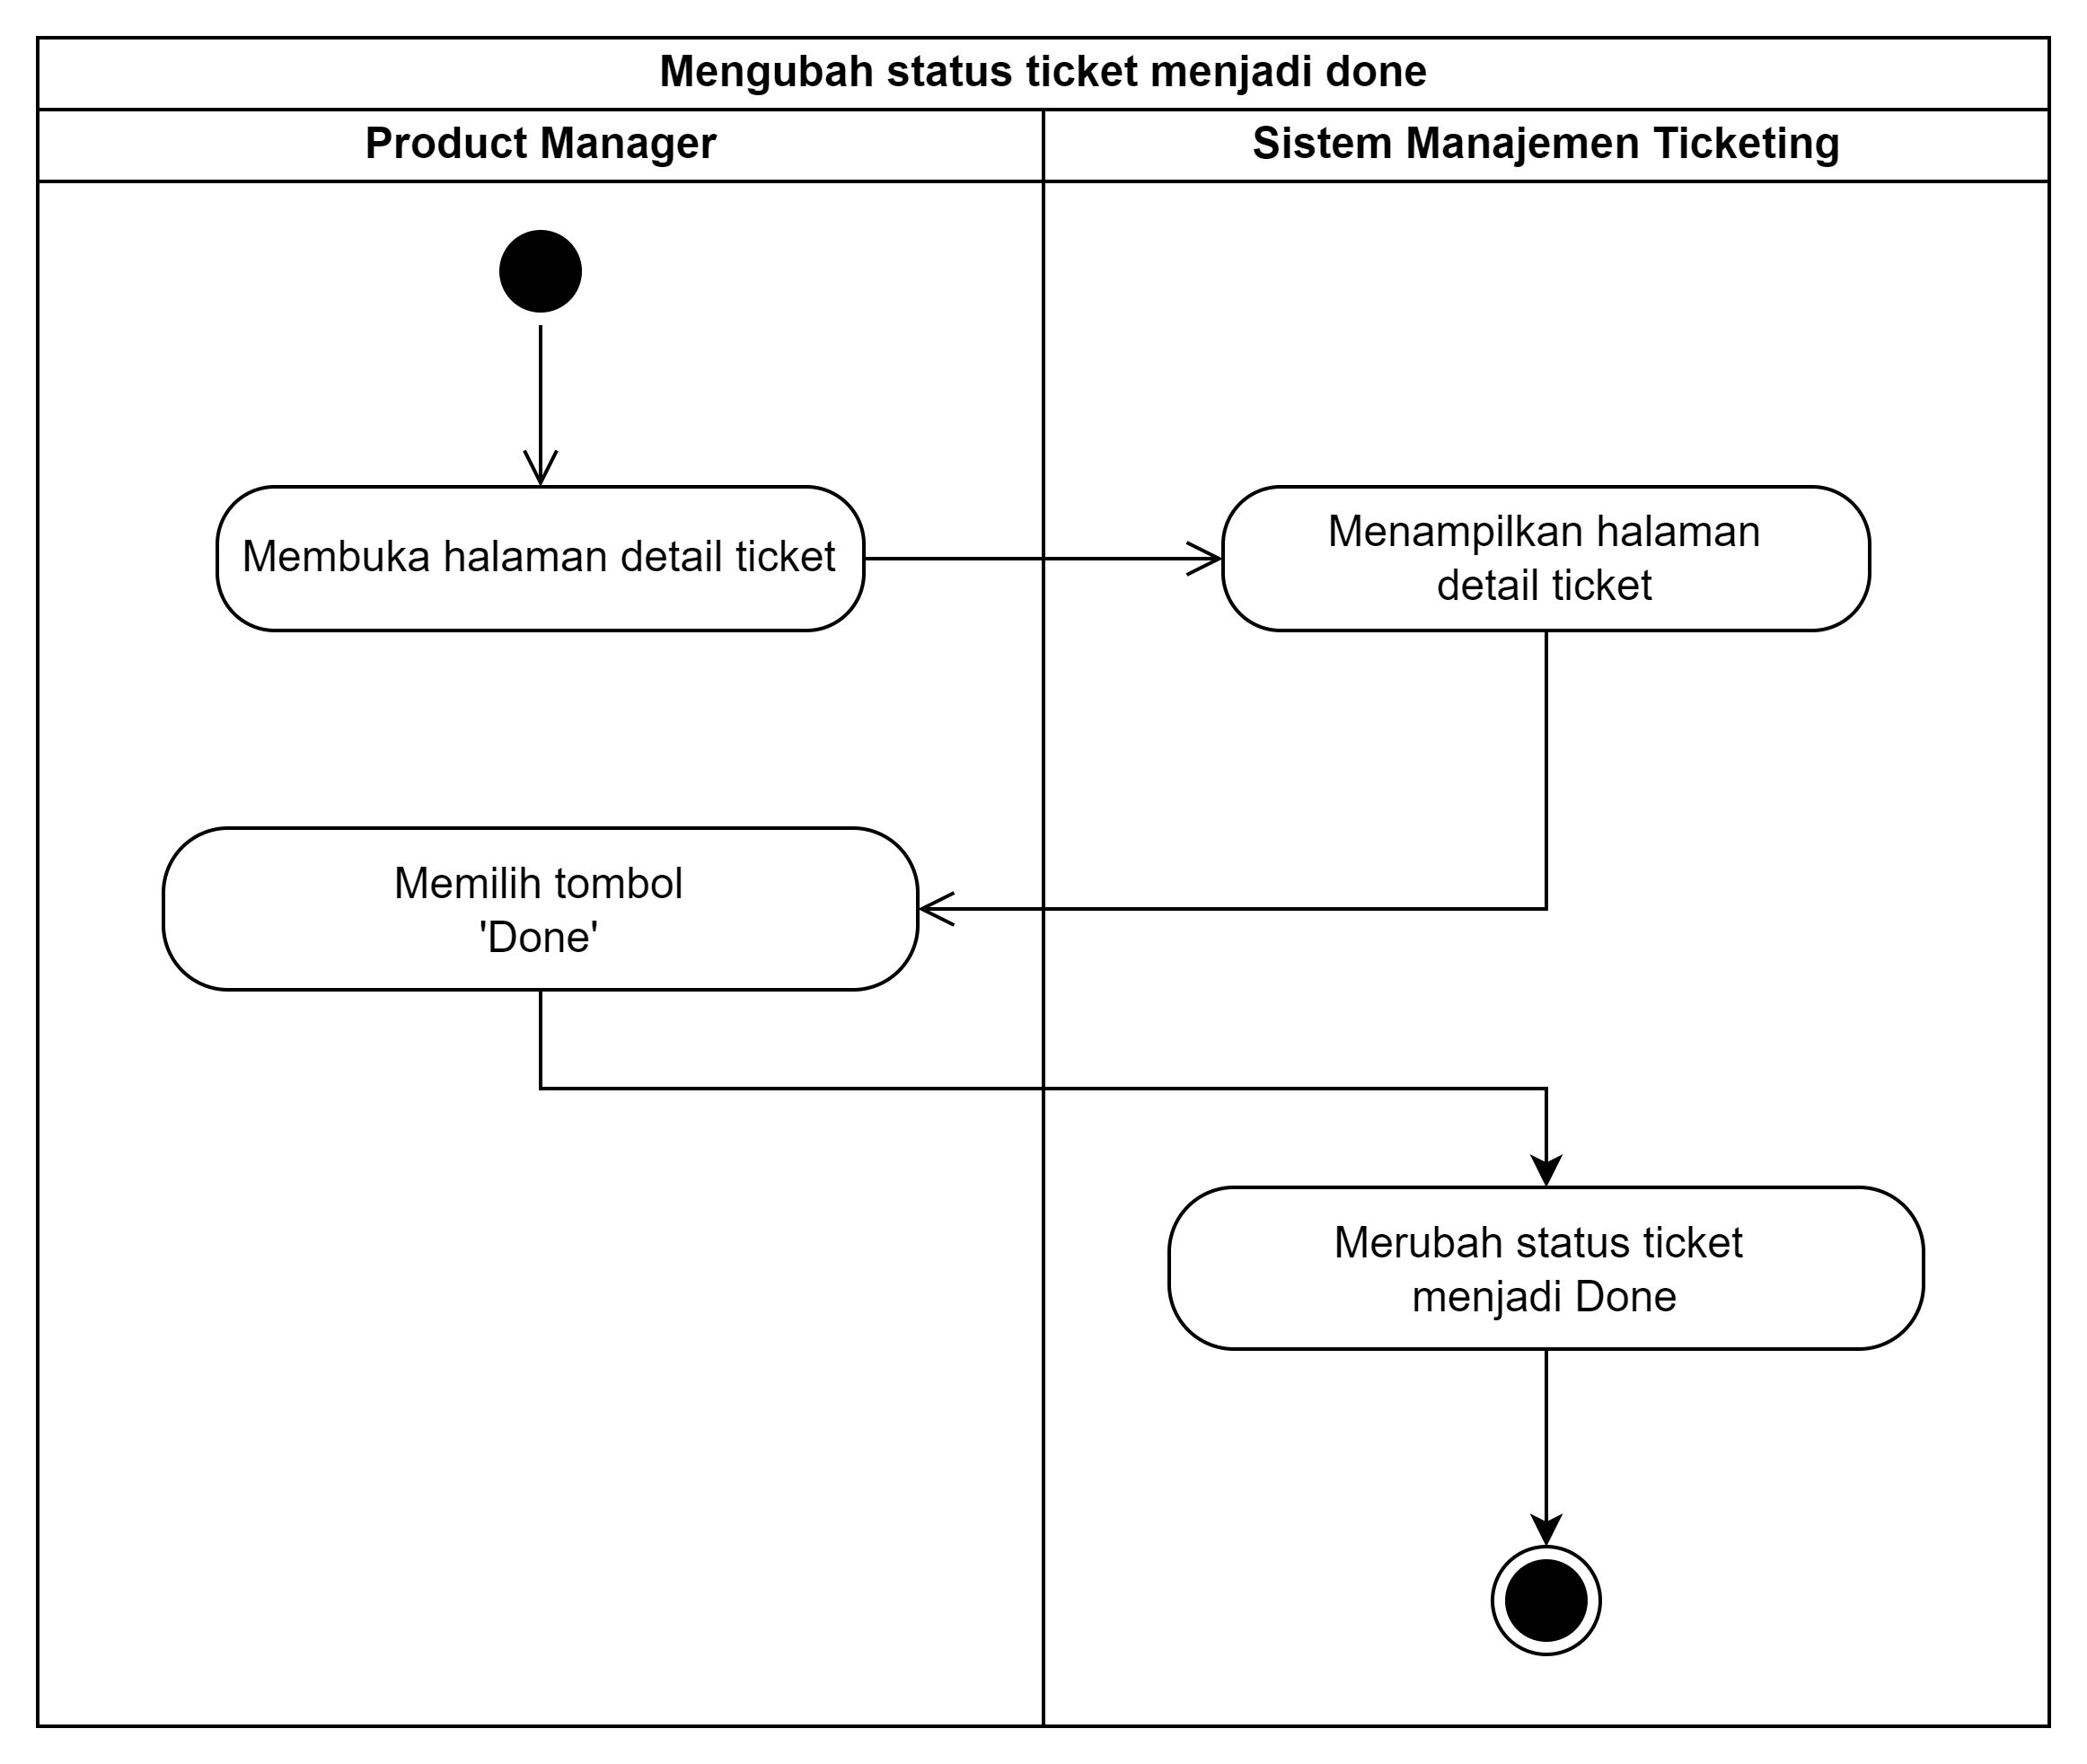
\includegraphics[width=0.75\textwidth]{images/activity/ipm/Mengubah Status Ticket Menjadi Done.png}
                    \caption{Activity Diagram Mengubah Status Ticket Menjadi Done (PM)}
                    \label{fig:AD-PM-08}
                \end{figure}
            \end{enumerate}
            
            \listsection{Activity Diagram Internal User (Developer)}
            
            \begin{enumerate}[label=\arabic*.,wide,labelindent=27pt]
                \item Activity Diagram Melihat List Ticket
                
                \hspace*{10pt}
                \begin{tabularx}{.9\linewidth}{@{} l l X @{}}
                    ID Activity & : & AD-DEV-01 \\

                    Deskripsi &	: & Activity Diagram berikut merupakan sebuah proses aktivitas yang dilakukan untuk melihat list ticket oleh internal user dengan role developer yang ditunjukkan pada gambar \ref{fig:AD-DEV-01}.
                \end{tabularx}
                \begin{figure}[H]
                    \centering 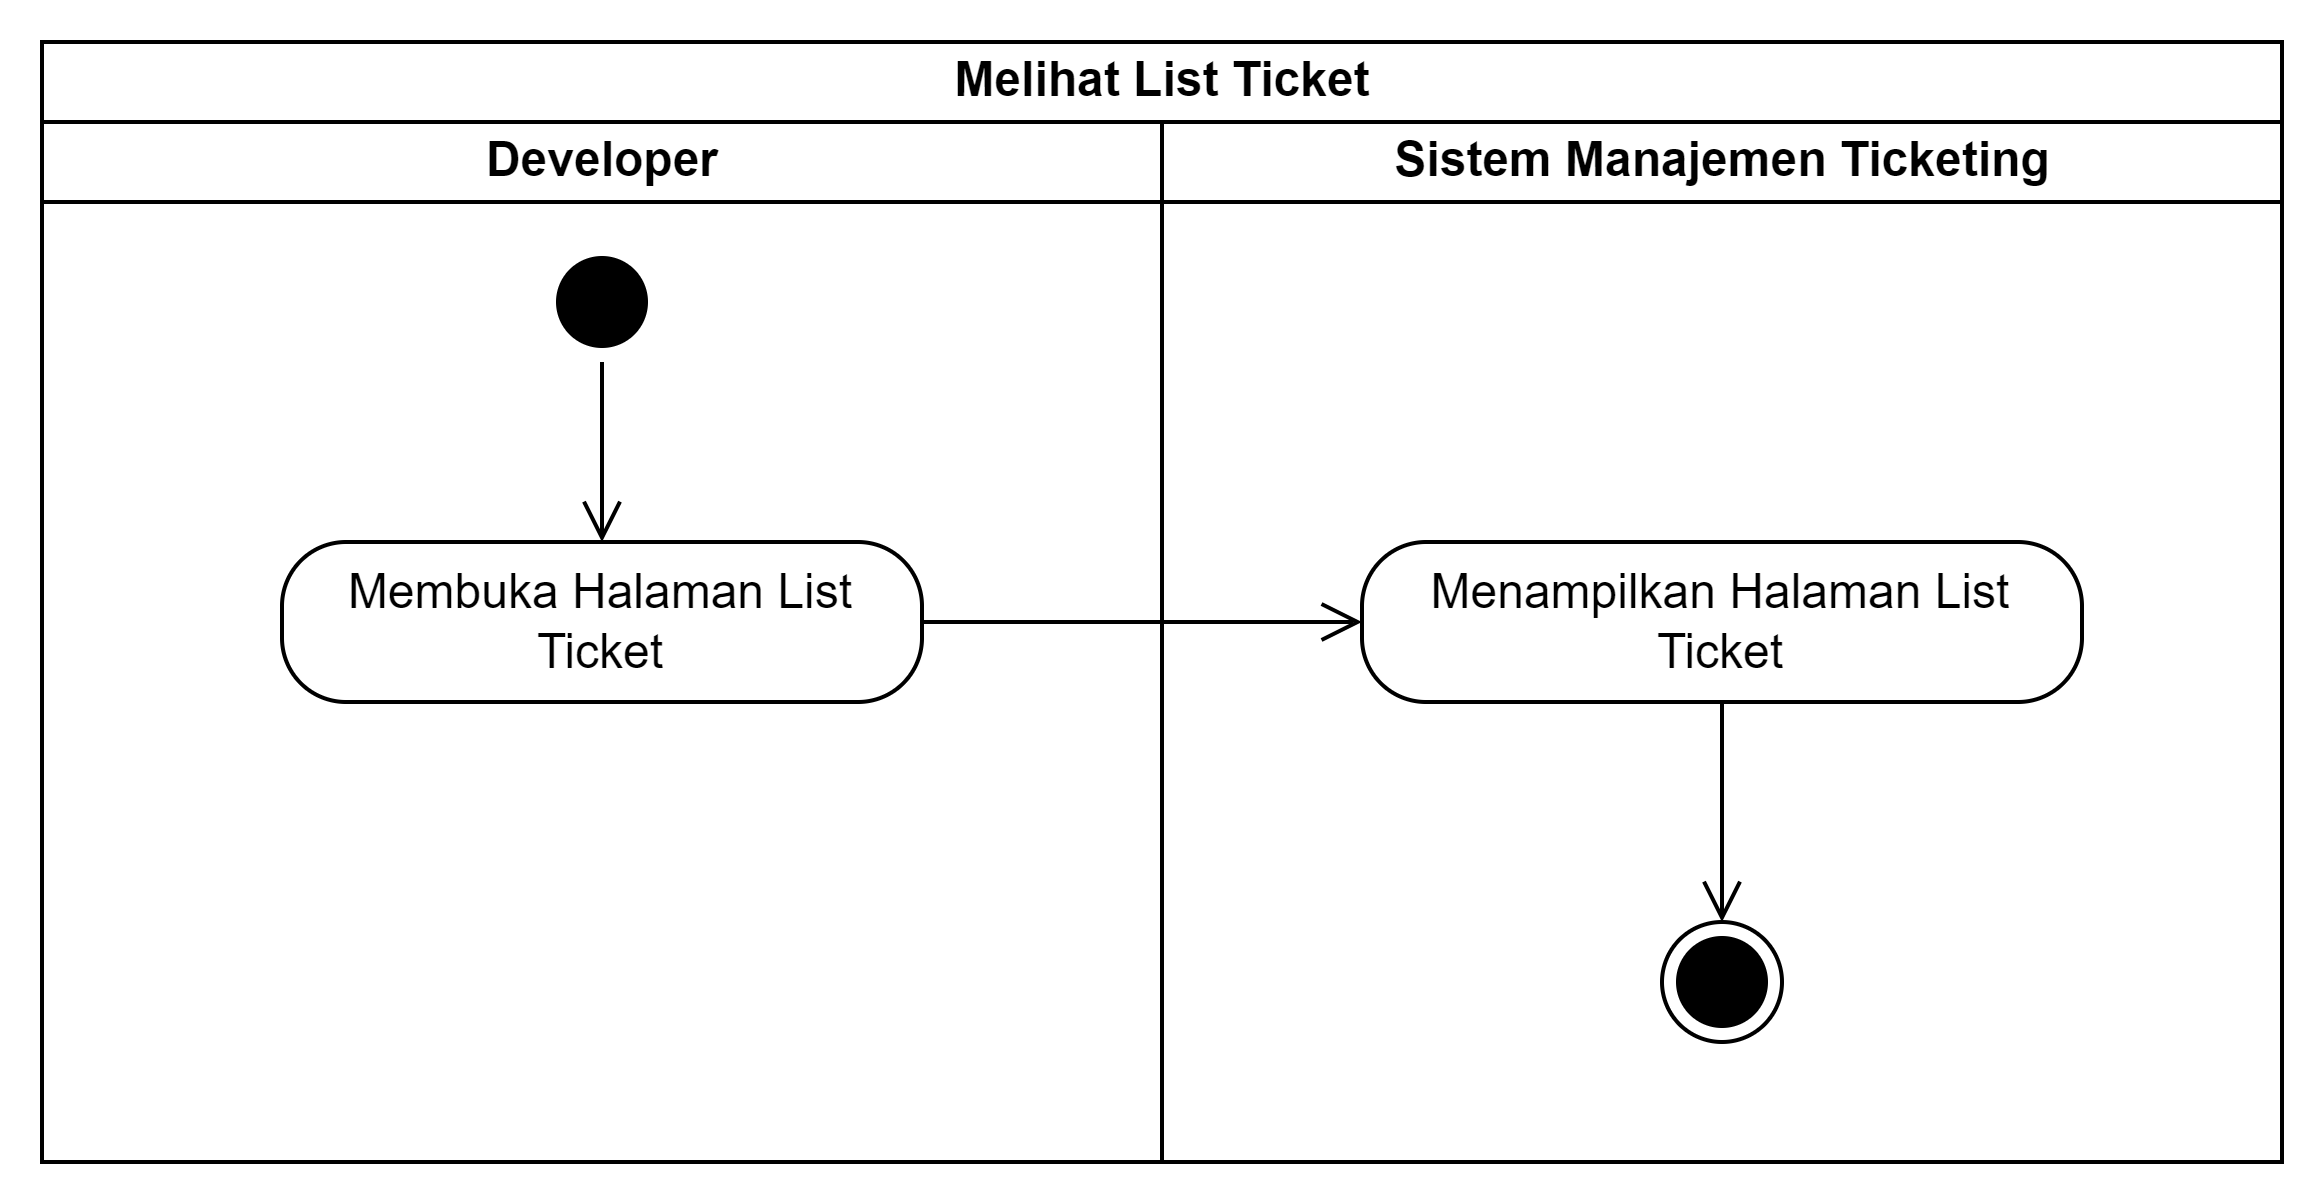
\includegraphics[width=0.75\textwidth]{images/activity/idev/Melihat List Ticket.png}
                    \caption{Activity Diagram Melihat List Ticket (DEV)}
                    \label{fig:AD-DEV-01}
                \end{figure}

                \item Activity Diagram Memfilter Ticket

                \hspace*{10pt}
                \begin{tabularx}{.9\linewidth}{@{} l l X @{}}
                    ID Activity & : & AD-DEV-02 \\

                    Deskripsi &	: & Activity Diagram berikut merupakan sebuah proses aktivitas yang dilakukan untuk memfilter list ticket oleh internal user dengan role developer yang ditunjukkan pada gambar \ref{fig:AD-DEV-02}.
                \end{tabularx}

                \begin{figure}[H]
                    \centering 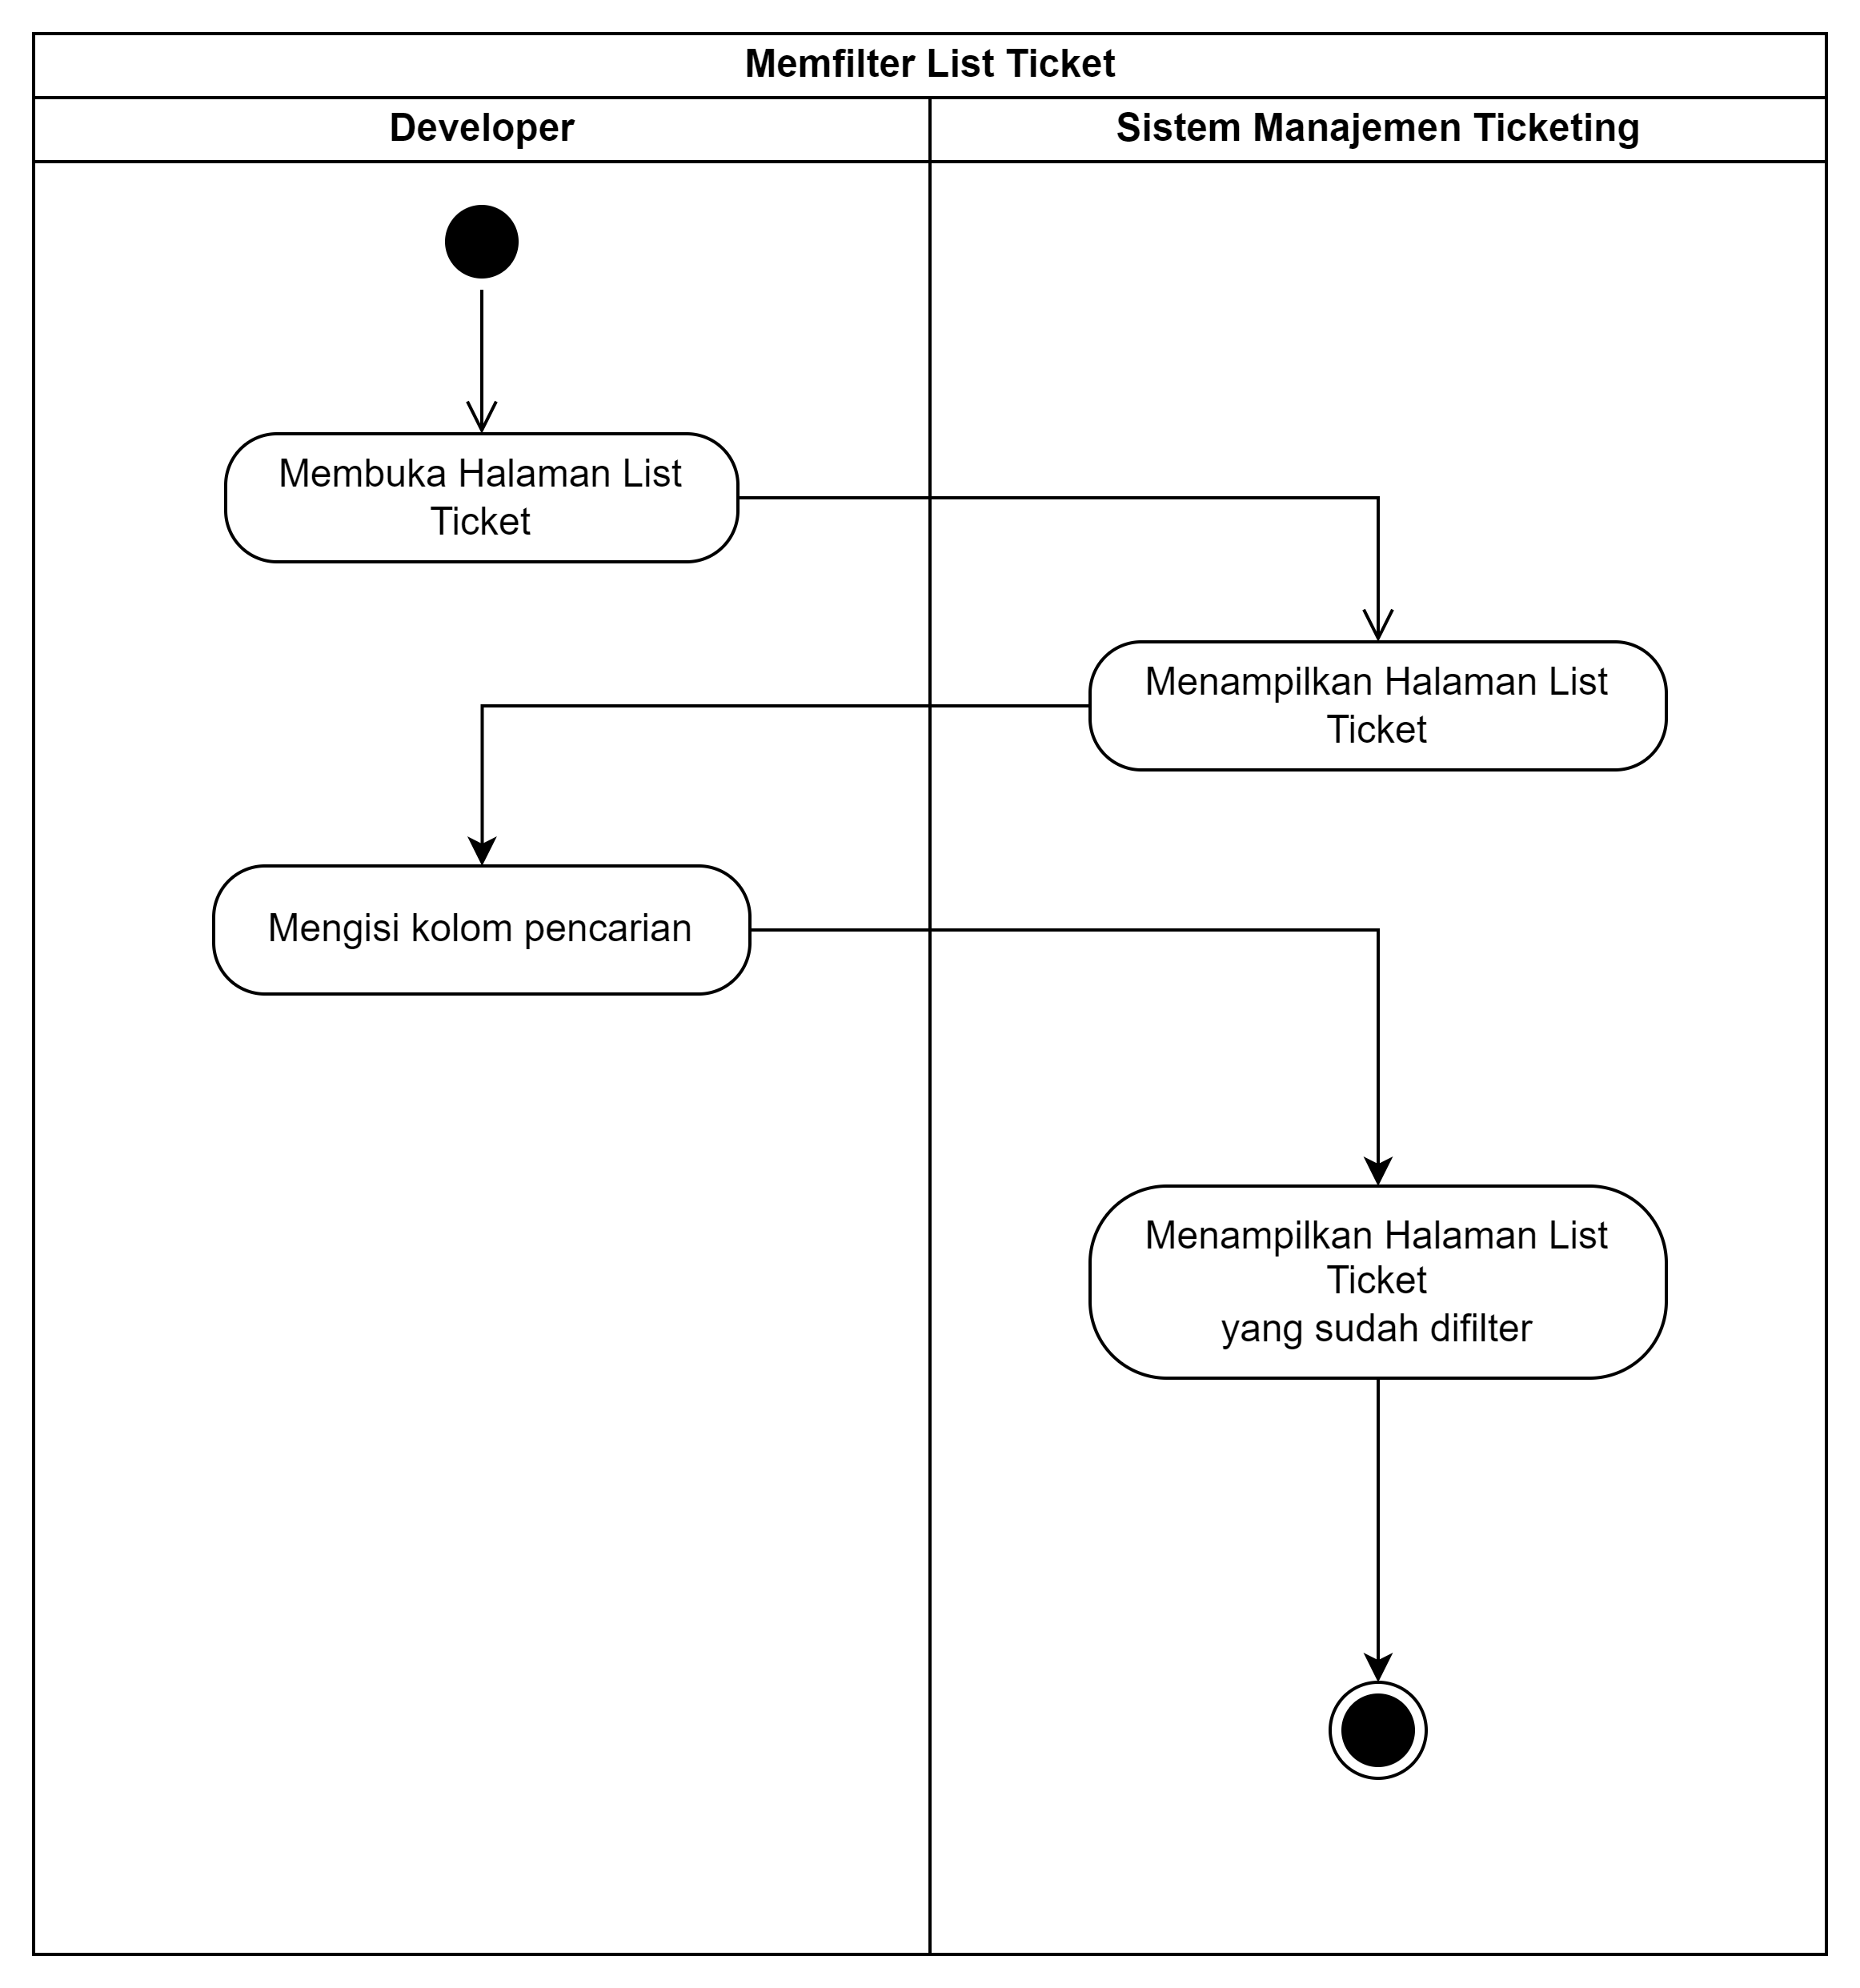
\includegraphics[width=0.75\textwidth]{images/activity/idev/Memfilter List Ticket.png}
                    \caption{Activity Diagram Memfilter List Ticket (DEV)}
                    \label{fig:AD-DEV-02}
                \end{figure}

                \item Activity Diagram Melihat Detail Ticket

                \hspace*{10pt}
                \begin{tabularx}{.9\linewidth}{@{} l l X @{}}
                    ID Activity & : & AD-DEV-03 \\

                    Deskripsi &	: & Activity Diagram berikut merupakan sebuah proses aktivitas yang dilakukan untuk melihat detail ticket oleh internal user dengan role developer yang ditunjukkan pada gambar \ref{fig:AD-DEV-03}.
                \end{tabularx}

                \begin{figure}[H]
                    \centering 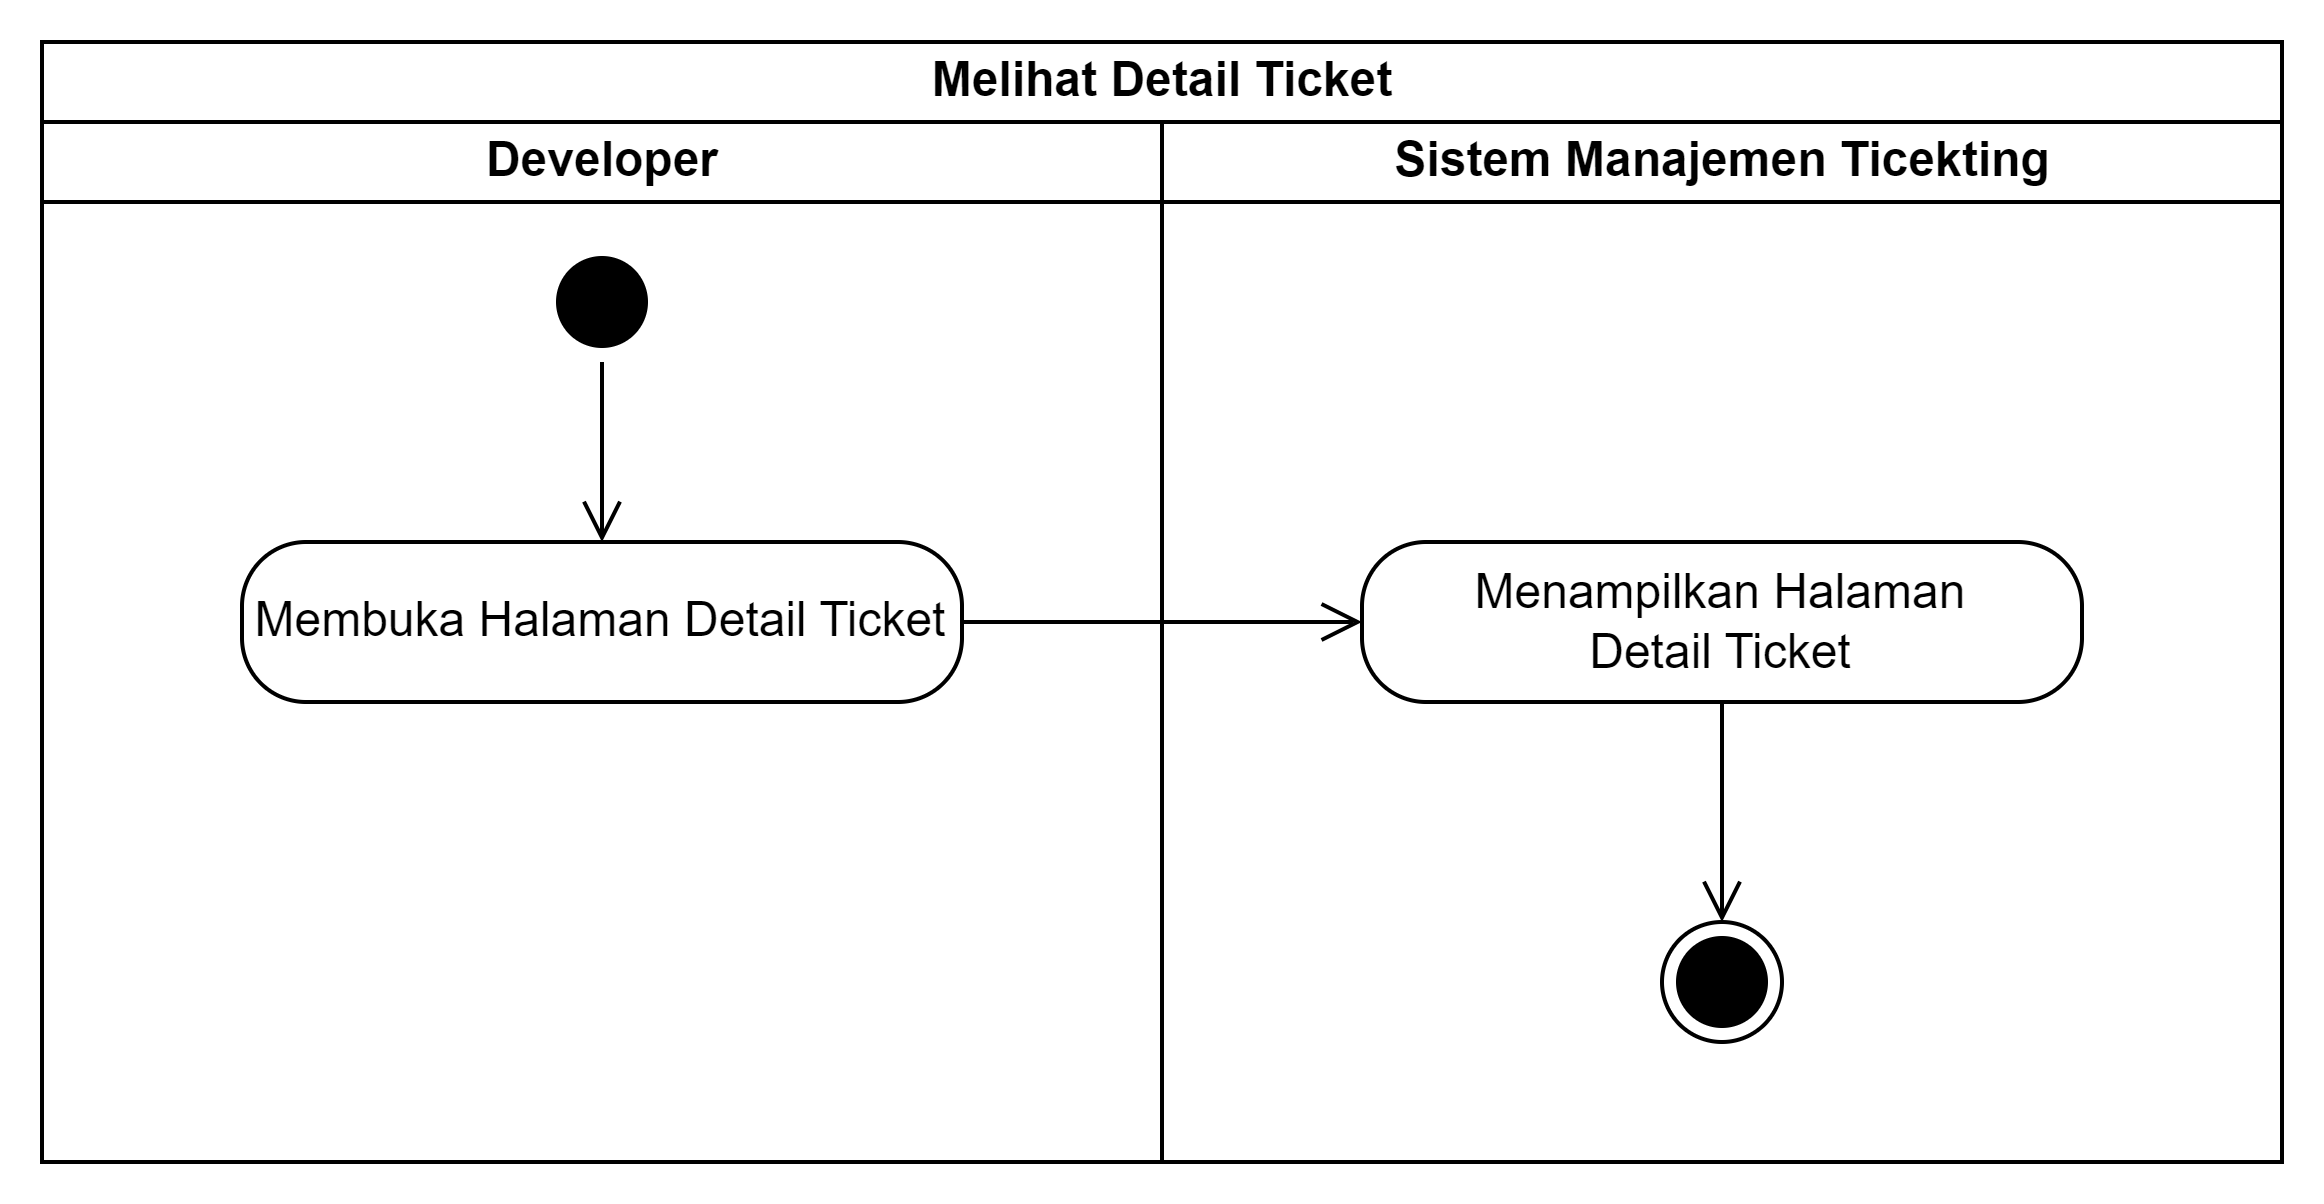
\includegraphics[width=0.75\textwidth]{images/activity/idev/Melihat Detail Ticket.png}
                    \caption{Activity Diagram Melihat Detail Ticket (DEV)}
                    \label{fig:AD-DEV-03}
                \end{figure}

                \item Activity Diagram Melaporkan Pekerjaan Ticket

                \hspace*{10pt}
                \begin{tabularx}{.9\linewidth}{@{} l l X @{}}
                    ID Activity & : & AD-DEV-04 \\

                    Deskripsi &	: & Activity Diagram berikut merupakan sebuah proses aktivitas yang dilakukan untuk melaporkan pengerjaan ticket oleh internal user dengan role developer yang ditunjukkan pada gambar \ref{fig:AD-DEV-04}.
                \end{tabularx}

                \begin{figure}[H]
                    \centering 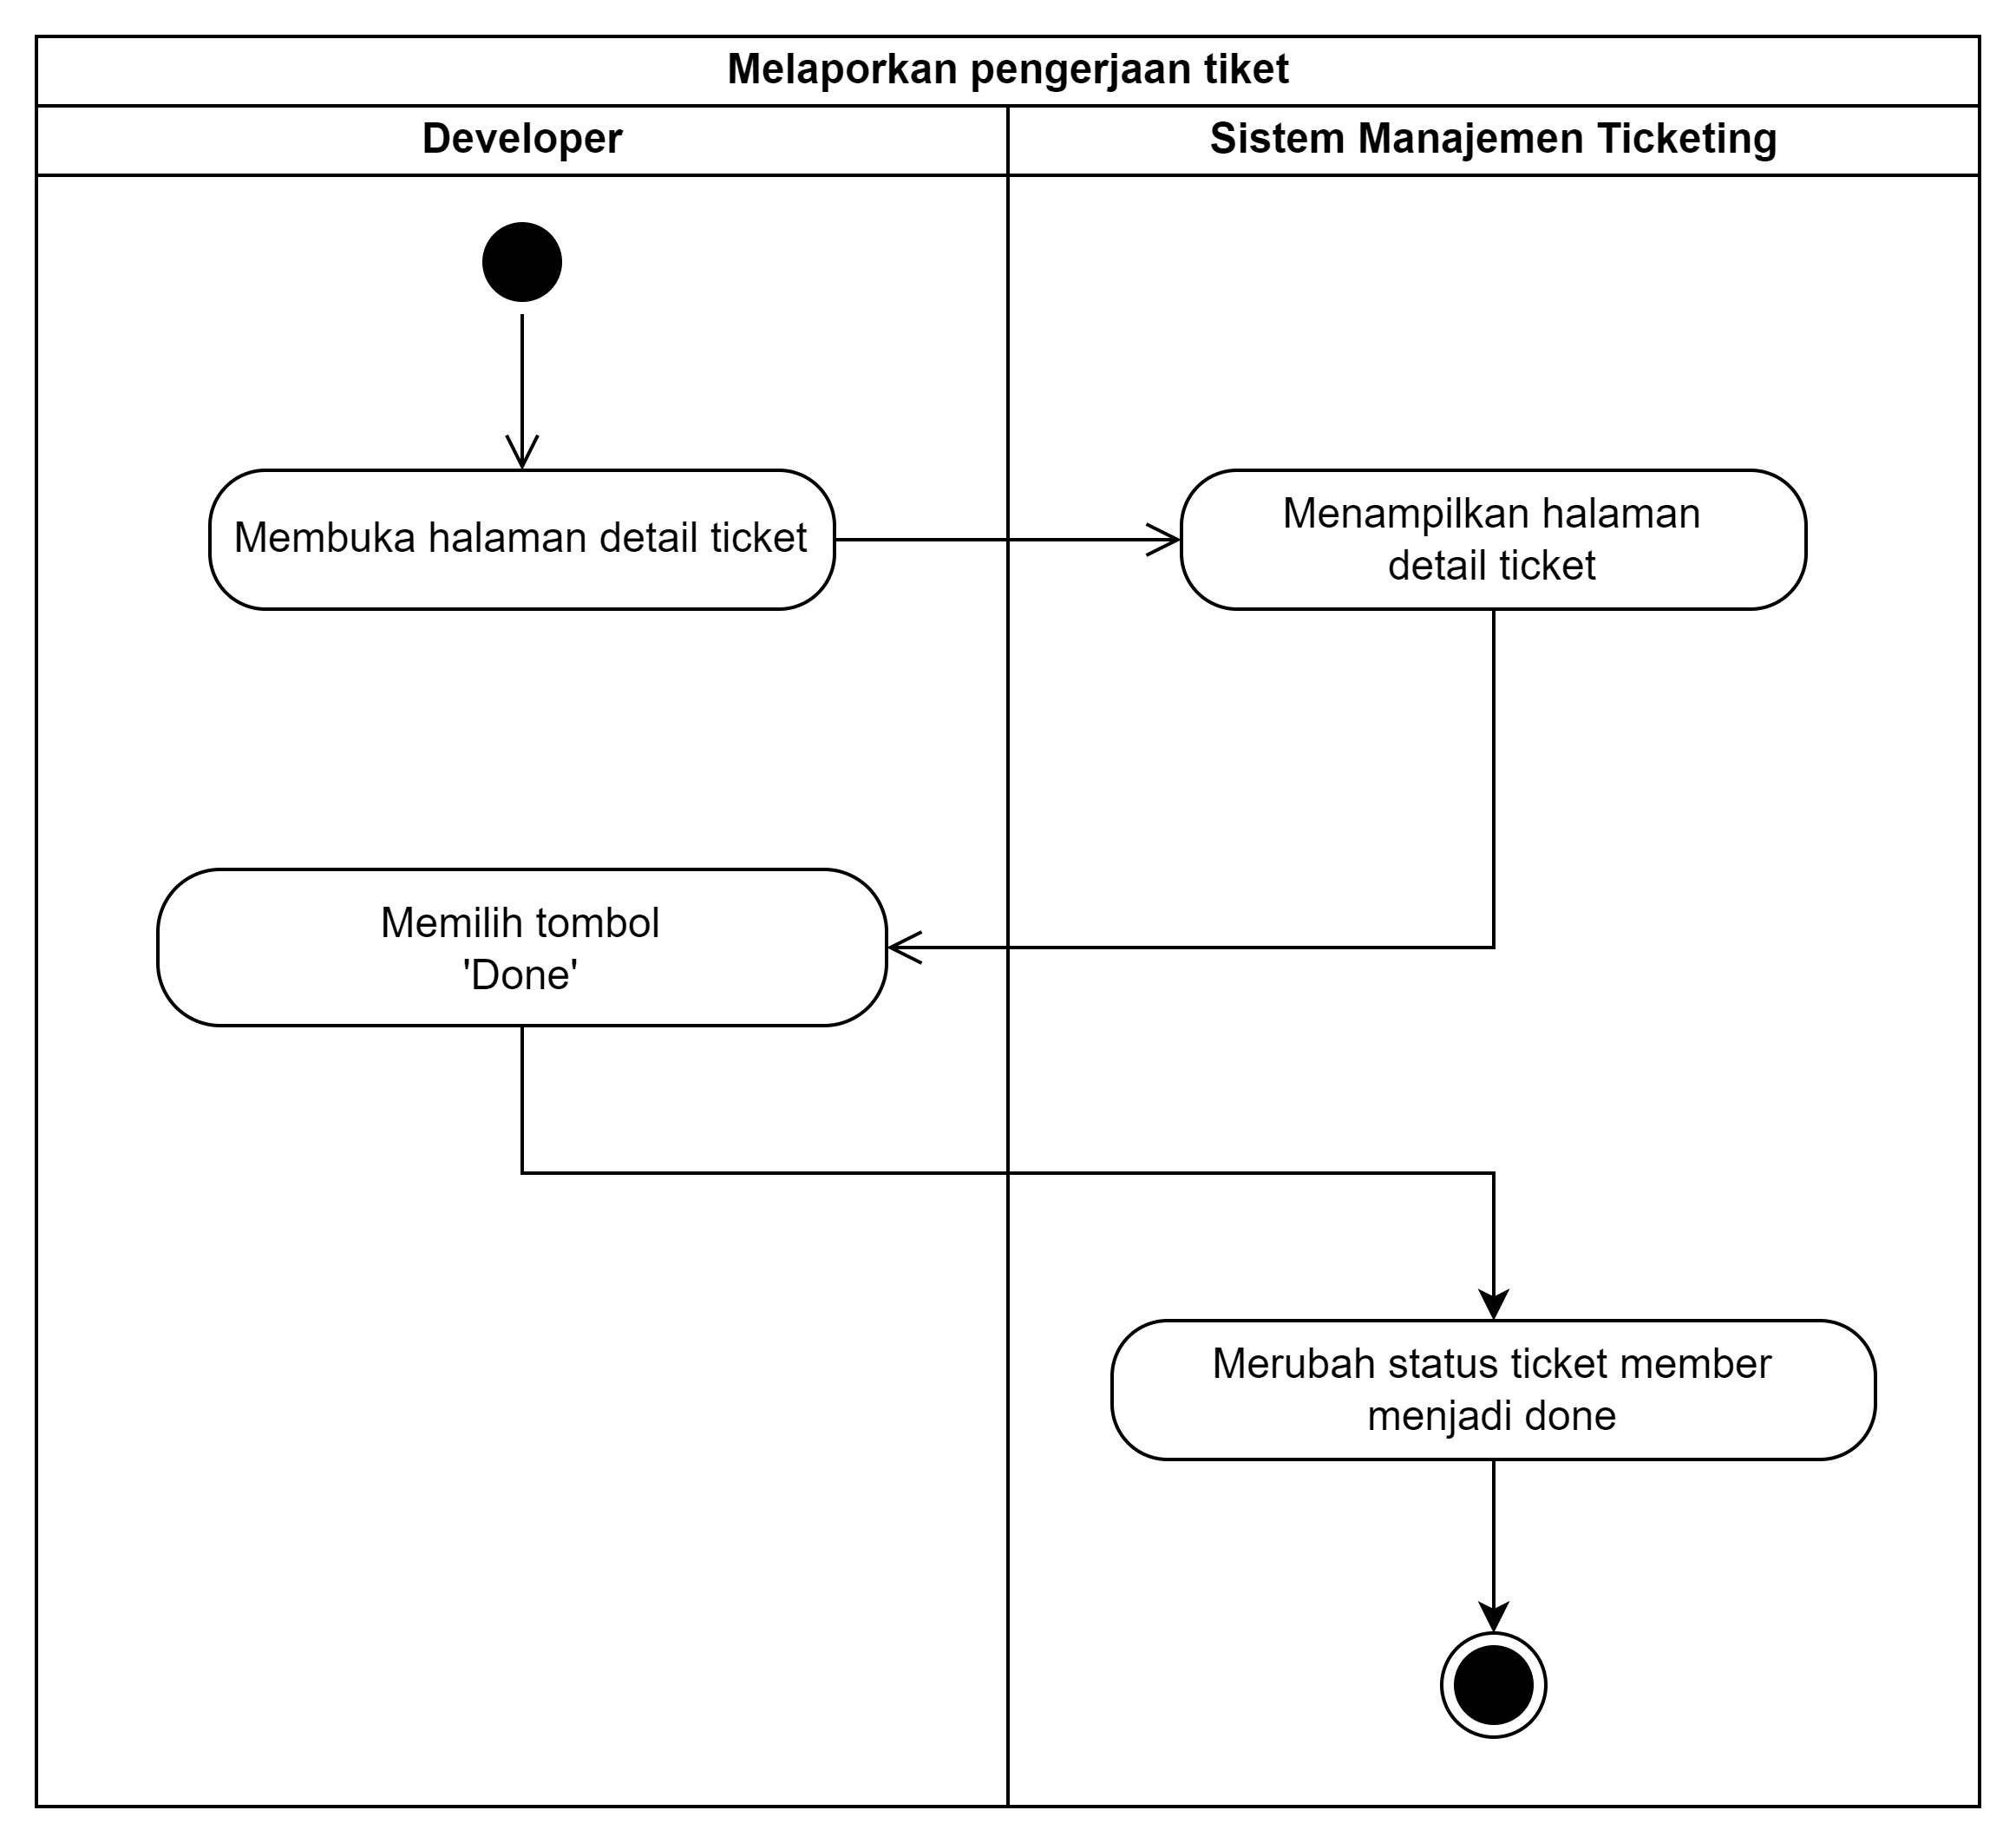
\includegraphics[width=0.75\textwidth]{images/activity/idev/Melaporkan Pengerjaan Ticket.png}
                    \caption{Activity Diagram Melaporkan Pengerjaan Ticket (DEV)}
                    \label{fig:AD-DEV-04}
                \end{figure}
            \end{enumerate}

            \listsection{Activity Diagram External User}
            \begin{enumerate}[label=\arabic*.,wide,labelindent=27pt]
                \item Activity Diagram Melihat List Ticket
                
                \hspace*{10pt}
                \begin{tabularx}{.9\linewidth}{@{} l l X @{}}
                    ID Activity & : & AD-PIC-01 \\

                    Deskripsi &	: & Activity Diagram berikut merupakan sebuah proses aktivitas yang dilakukan untuk melihat list ticket oleh seorang external user yang ditunjukkan pada gambar \ref{fig:AD-PIC-01}.
                \end{tabularx}
                
                \begin{figure}[H]
                    \centering 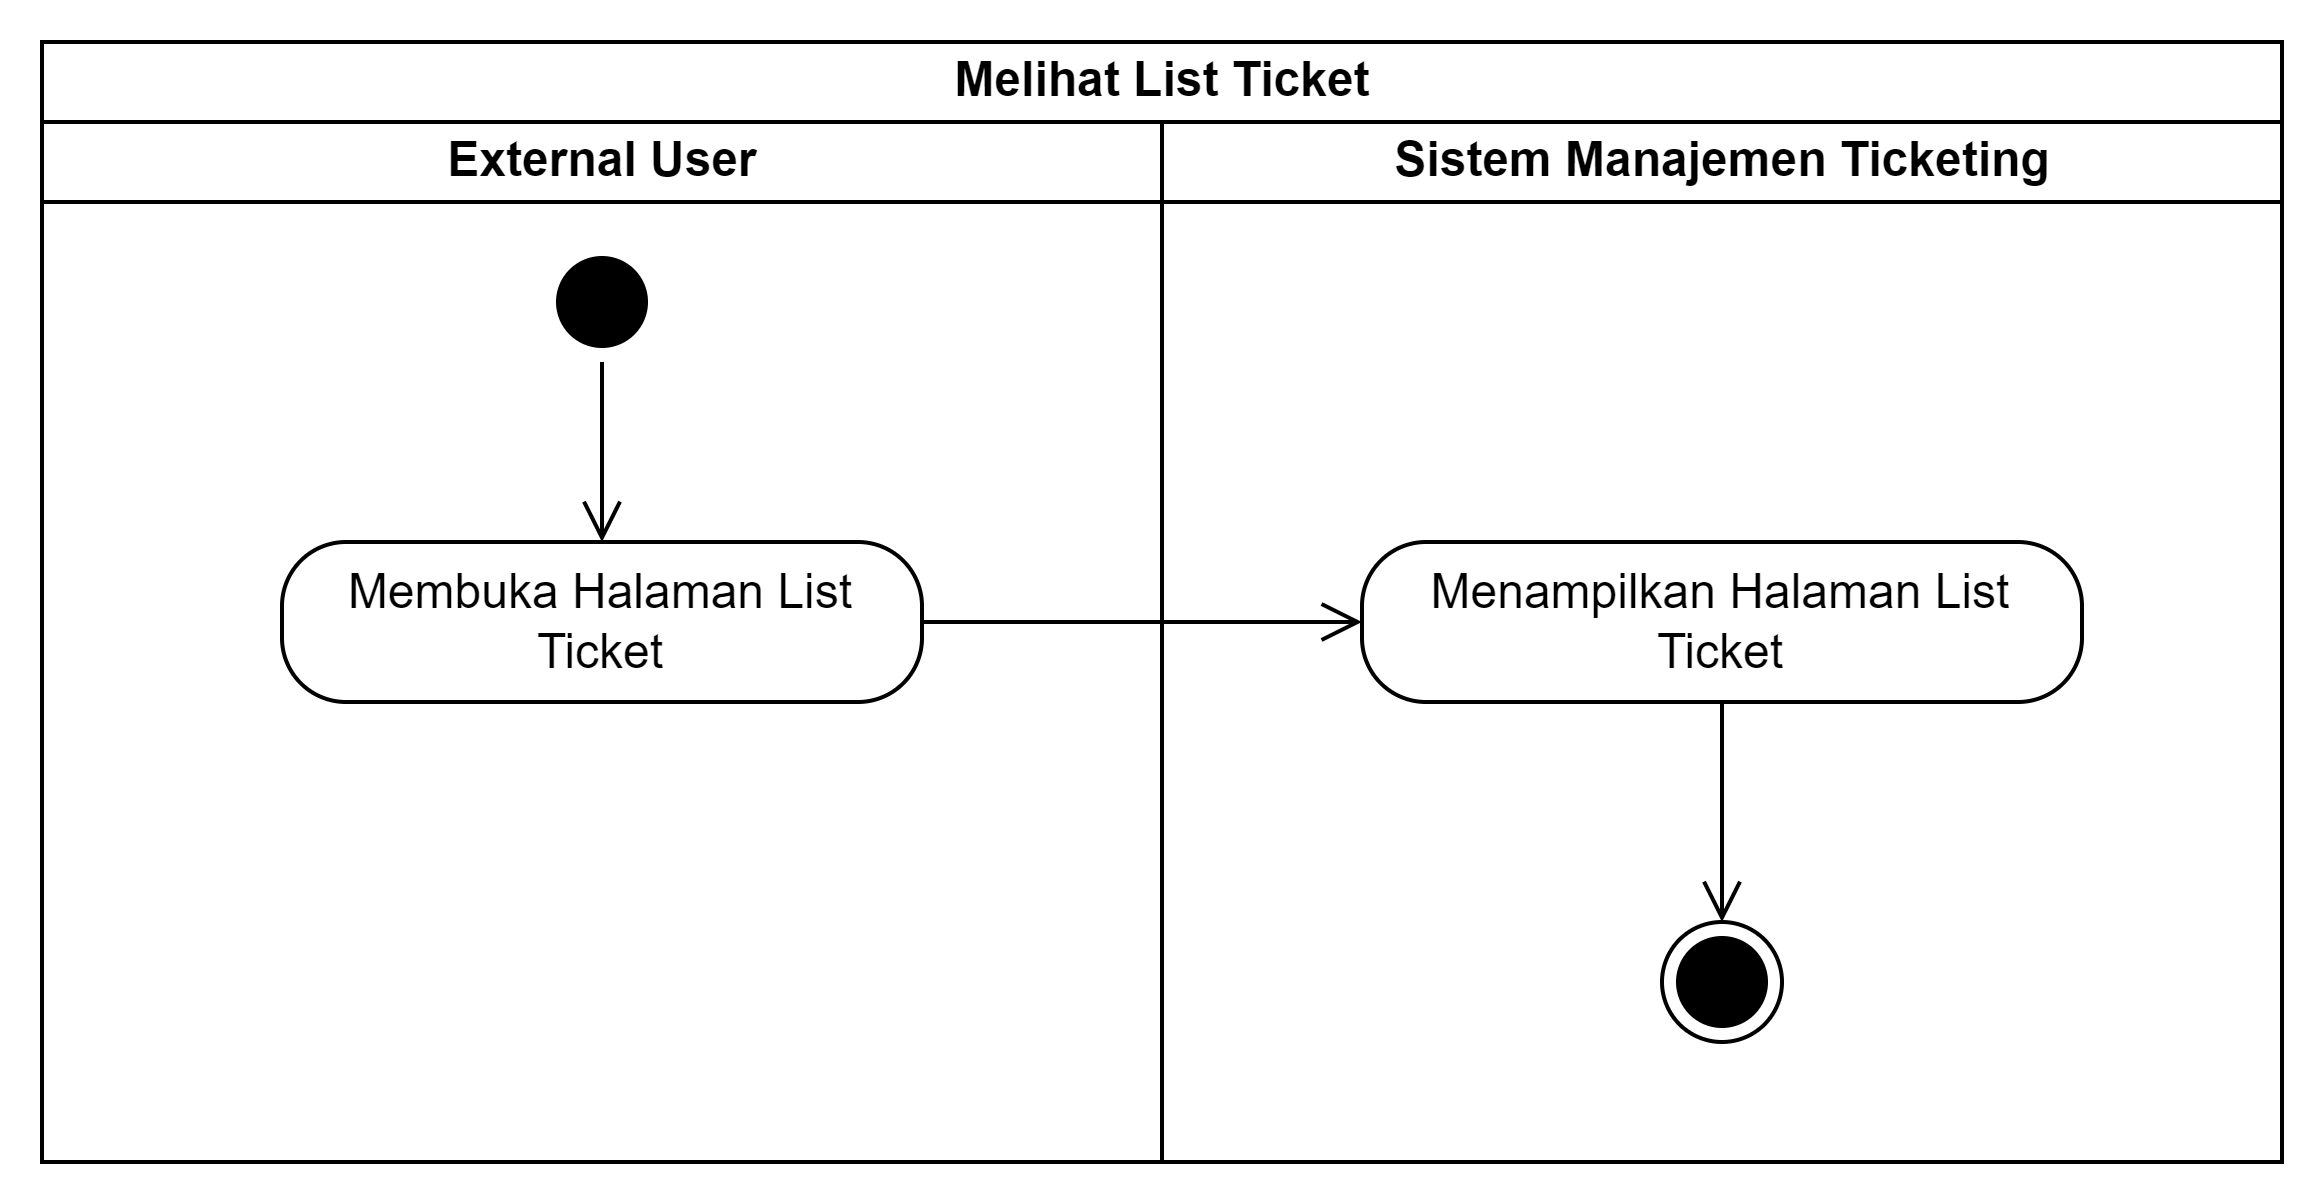
\includegraphics[width=0.75\textwidth]{images/activity/ex/Melihat List Ticket.png}
                    \caption{Activity Diagram Melihat List Ticket (External User)}
                    \label{fig:AD-PIC-01}
                \end{figure}

                \item Activity Diagram Memfilter List Ticket

                \hspace*{10pt}
                \begin{tabularx}{.9\linewidth}{@{} l l X @{}}
                    ID Activity & : & AD-PIC-02 \\

                    Deskripsi &	: & Activity Diagram berikut merupakan sebuah proses aktivitas yang dilakukan untuk memfilter ticket oleh seorang external user yang ditunjukkan pada gambar \ref{fig:AD-PIC-02}.
                \end{tabularx}

                \begin{figure}[H]
                    \centering 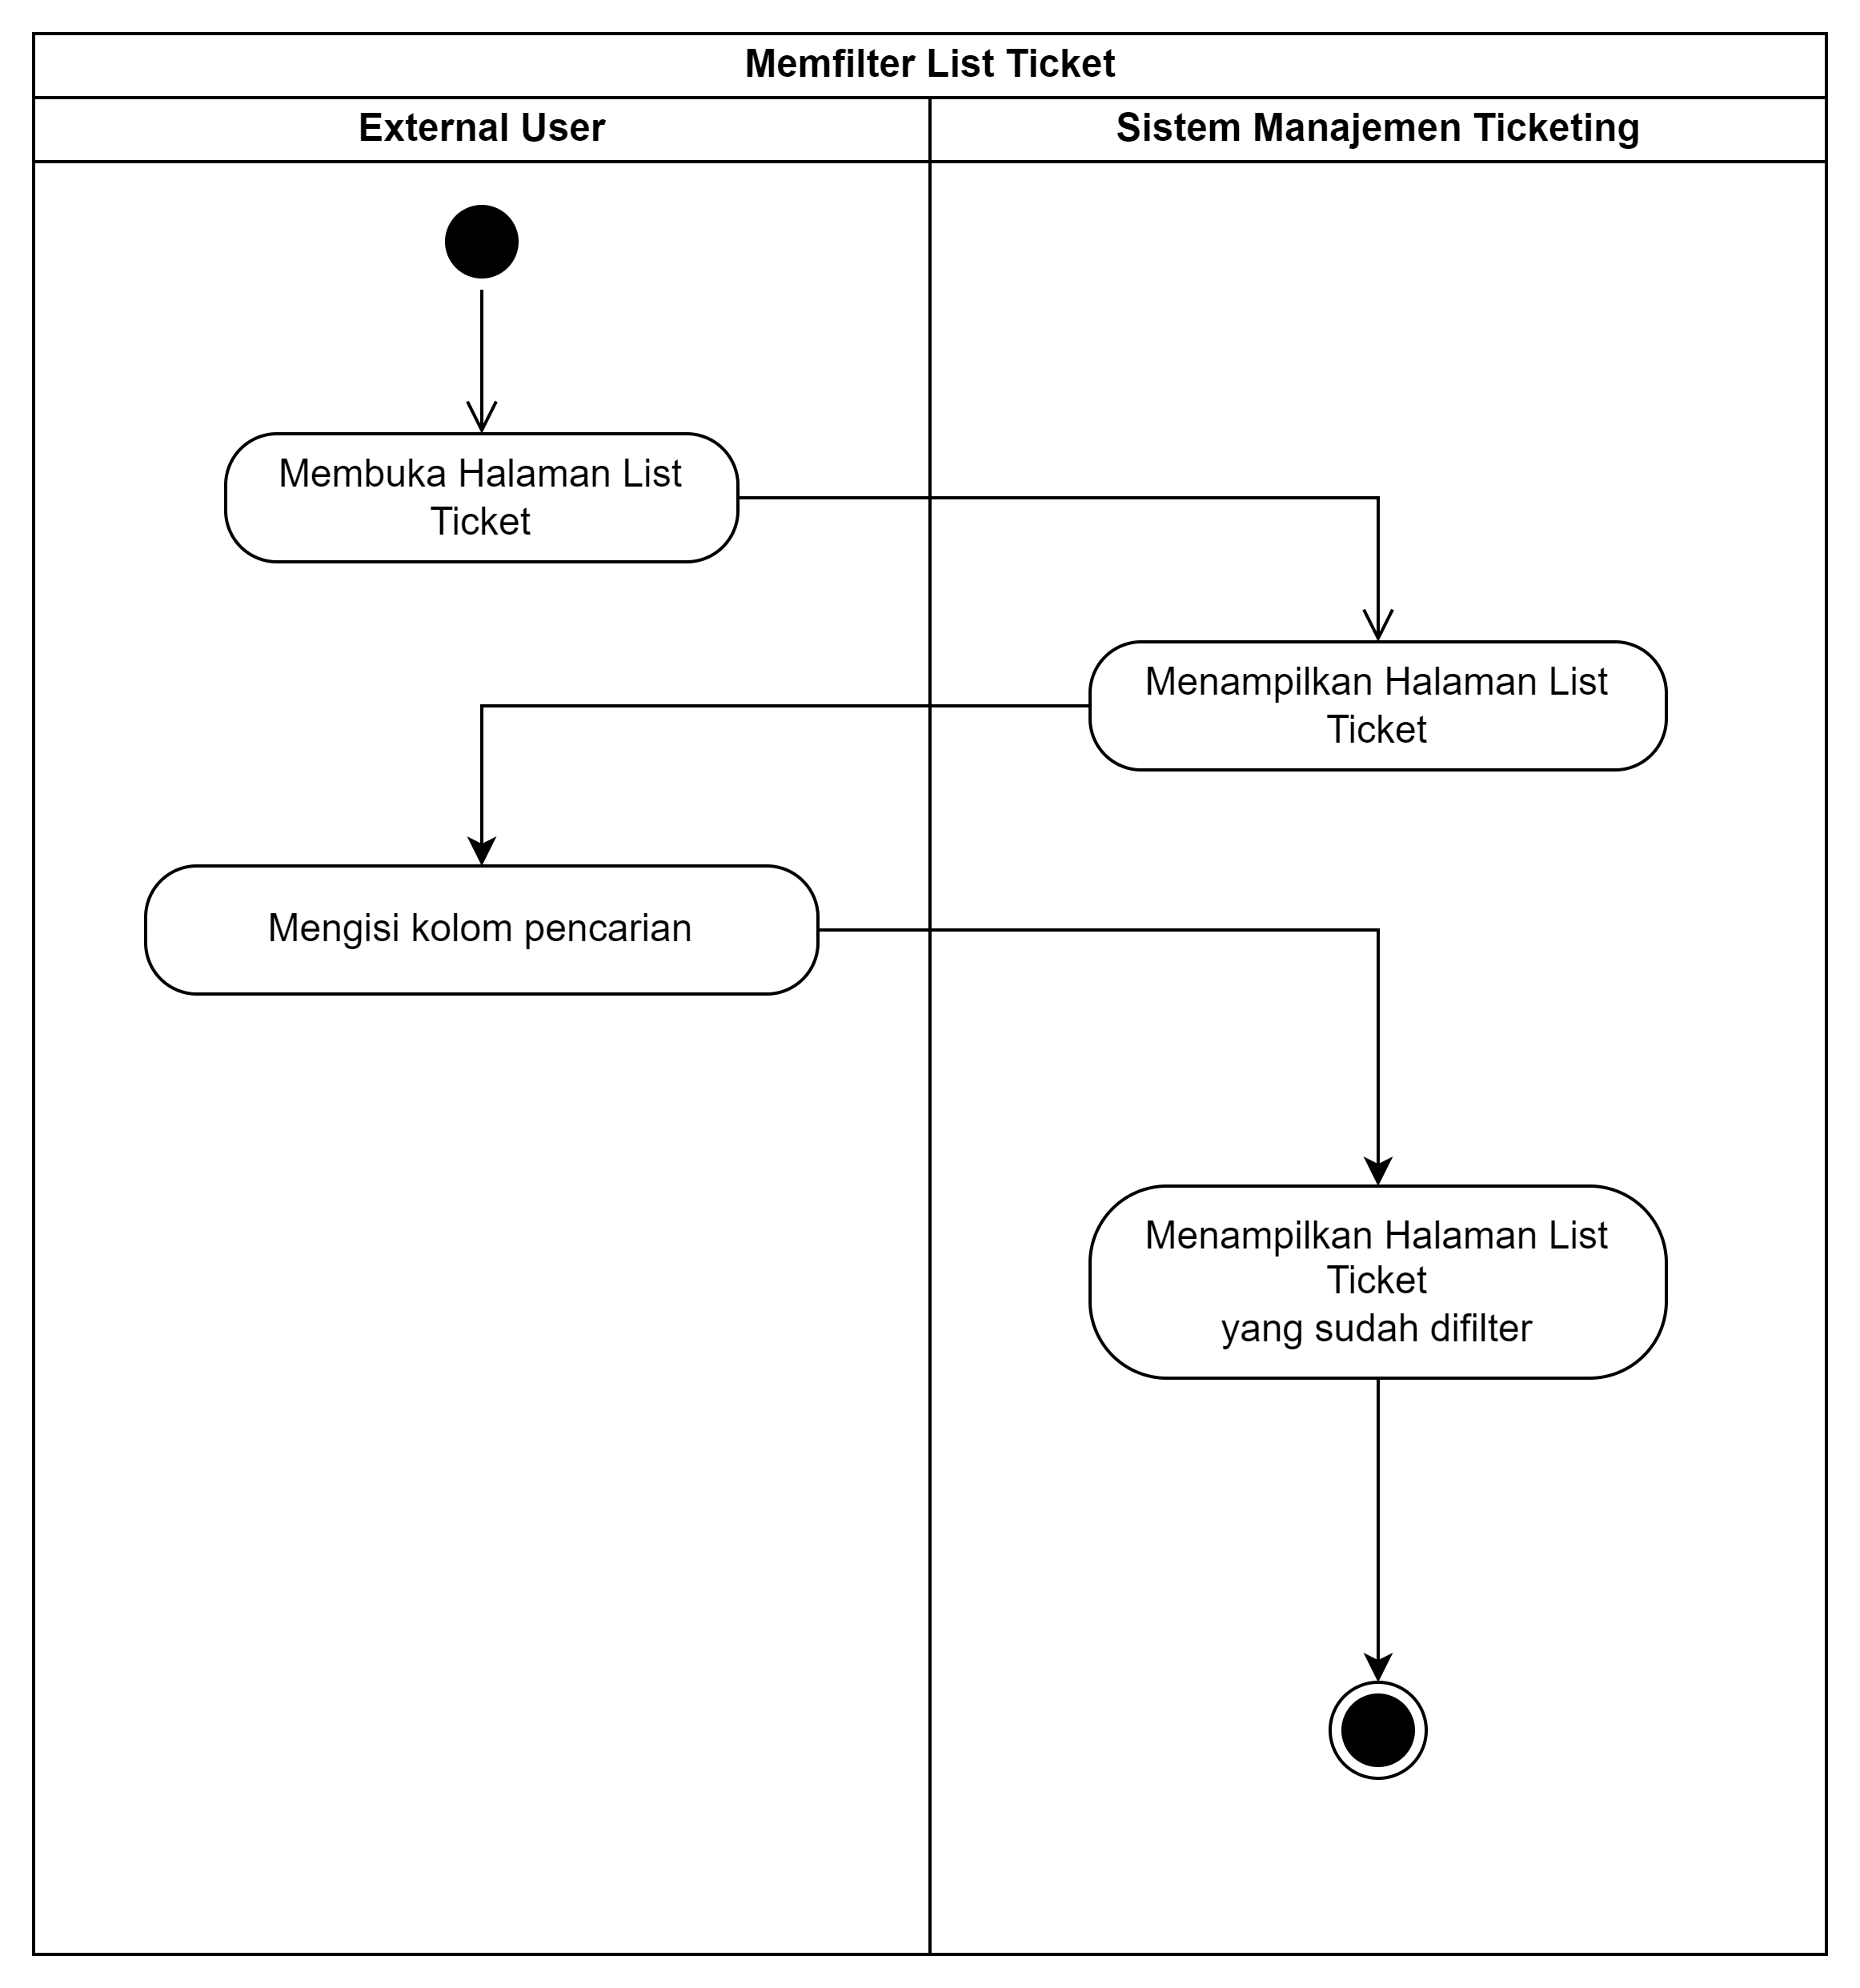
\includegraphics[width=0.75\textwidth]{images/activity/ex/Memfilter List Ticket.png}
                    \caption{Activity Diagram Memfilter List Ticket (External User)}
                    \label{fig:AD-PIC-02}
                \end{figure}

                \item Activity Diagram Membuat Ticket

                \hspace*{10pt}
                \begin{tabularx}{.9\linewidth}{@{} l l X @{}}
                    ID Activity & : & AD-PIC-03 \\

                    Deskripsi &	: & Activity Diagram berikut merupakan sebuah proses aktivitas yang dilakukan untuk membuat ticket oleh seorang external user yang ditunjukkan pada gambar \ref{fig:AD-PIC-03}.
                \end{tabularx}

                \begin{figure}[H]
                    \centering 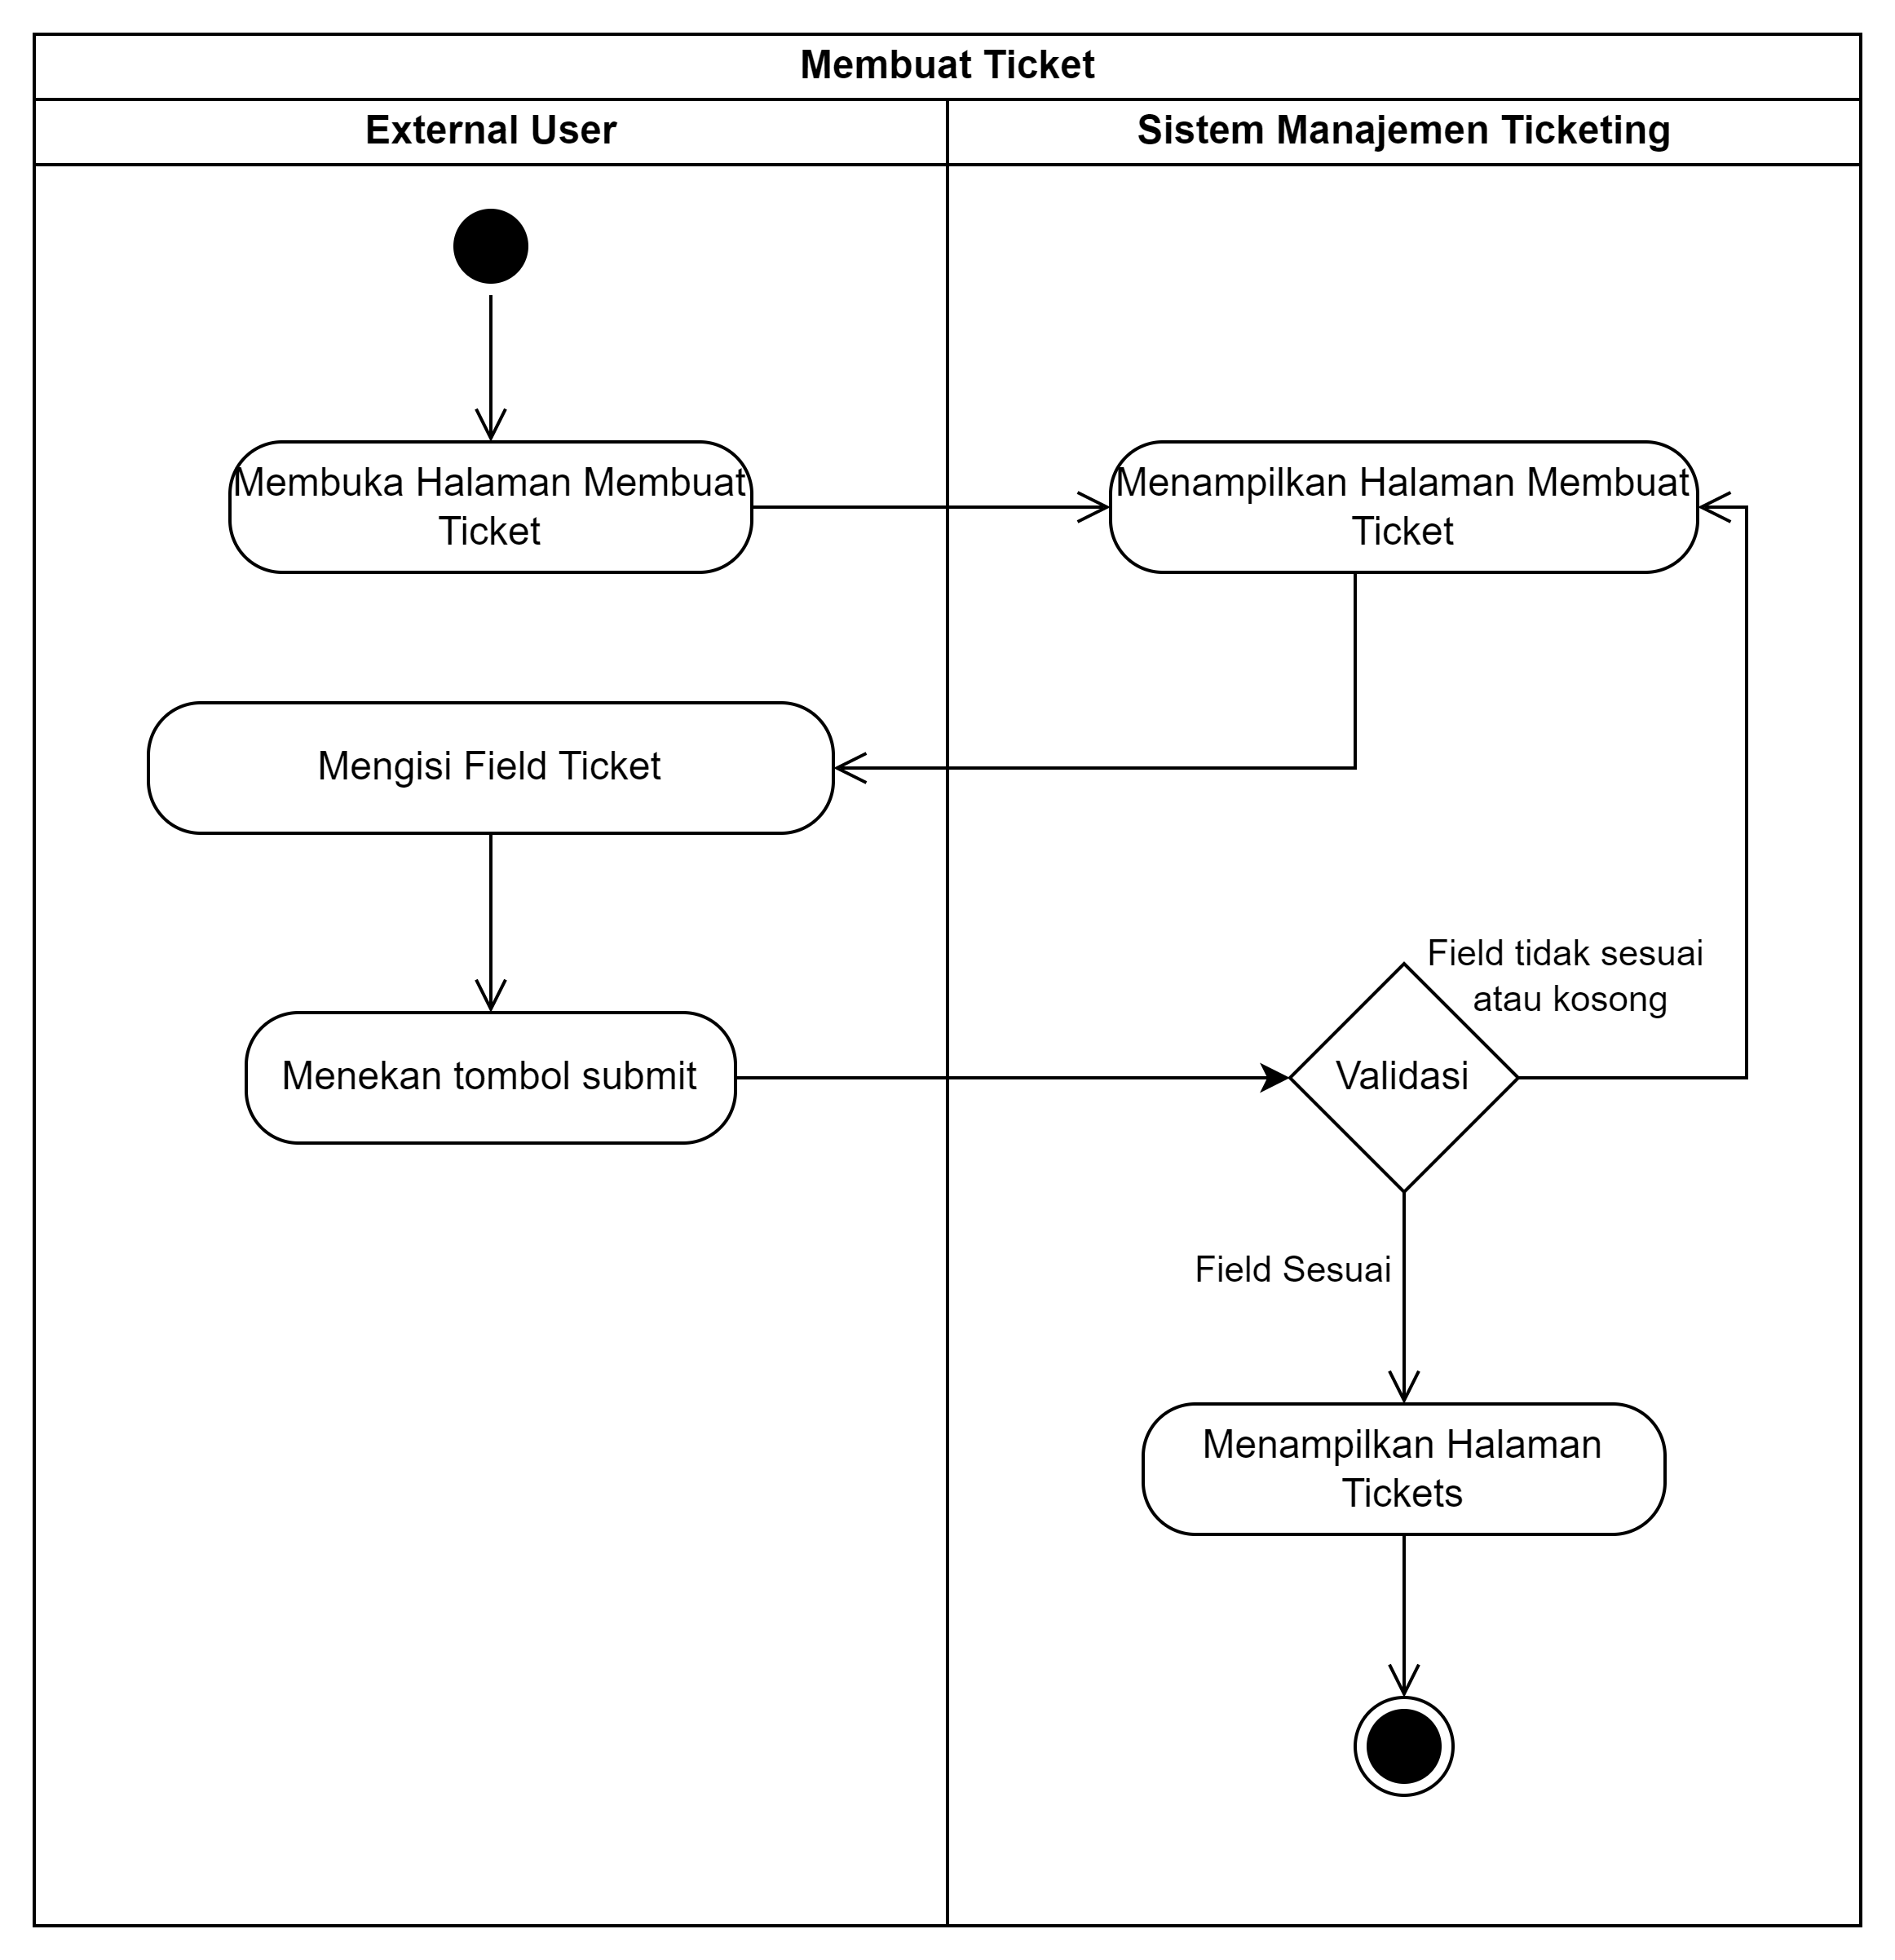
\includegraphics[width=0.75\textwidth]{images/activity/ex/Membuat Ticket.png}
                    \caption{Activity Diagram Membuat Ticket (External User)}
                    \label{fig:AD-PIC-03}
                \end{figure}

                \item Activity Diagram Melihat Detail Ticket

                \hspace*{10pt}
                \begin{tabularx}{.9\linewidth}{@{} l l X @{}}
                    ID Activity & : & AD-PIC-04 \\

                    Deskripsi &	: & Activity Diagram berikut merupakan sebuah proses aktivitas yang dilakukan untuk melihat detail ticket oleh seorang external user yang ditunjukkan pada gambar \ref{fig:AD-PIC-04}.
                \end{tabularx}

                \begin{figure}[H]
                    \centering 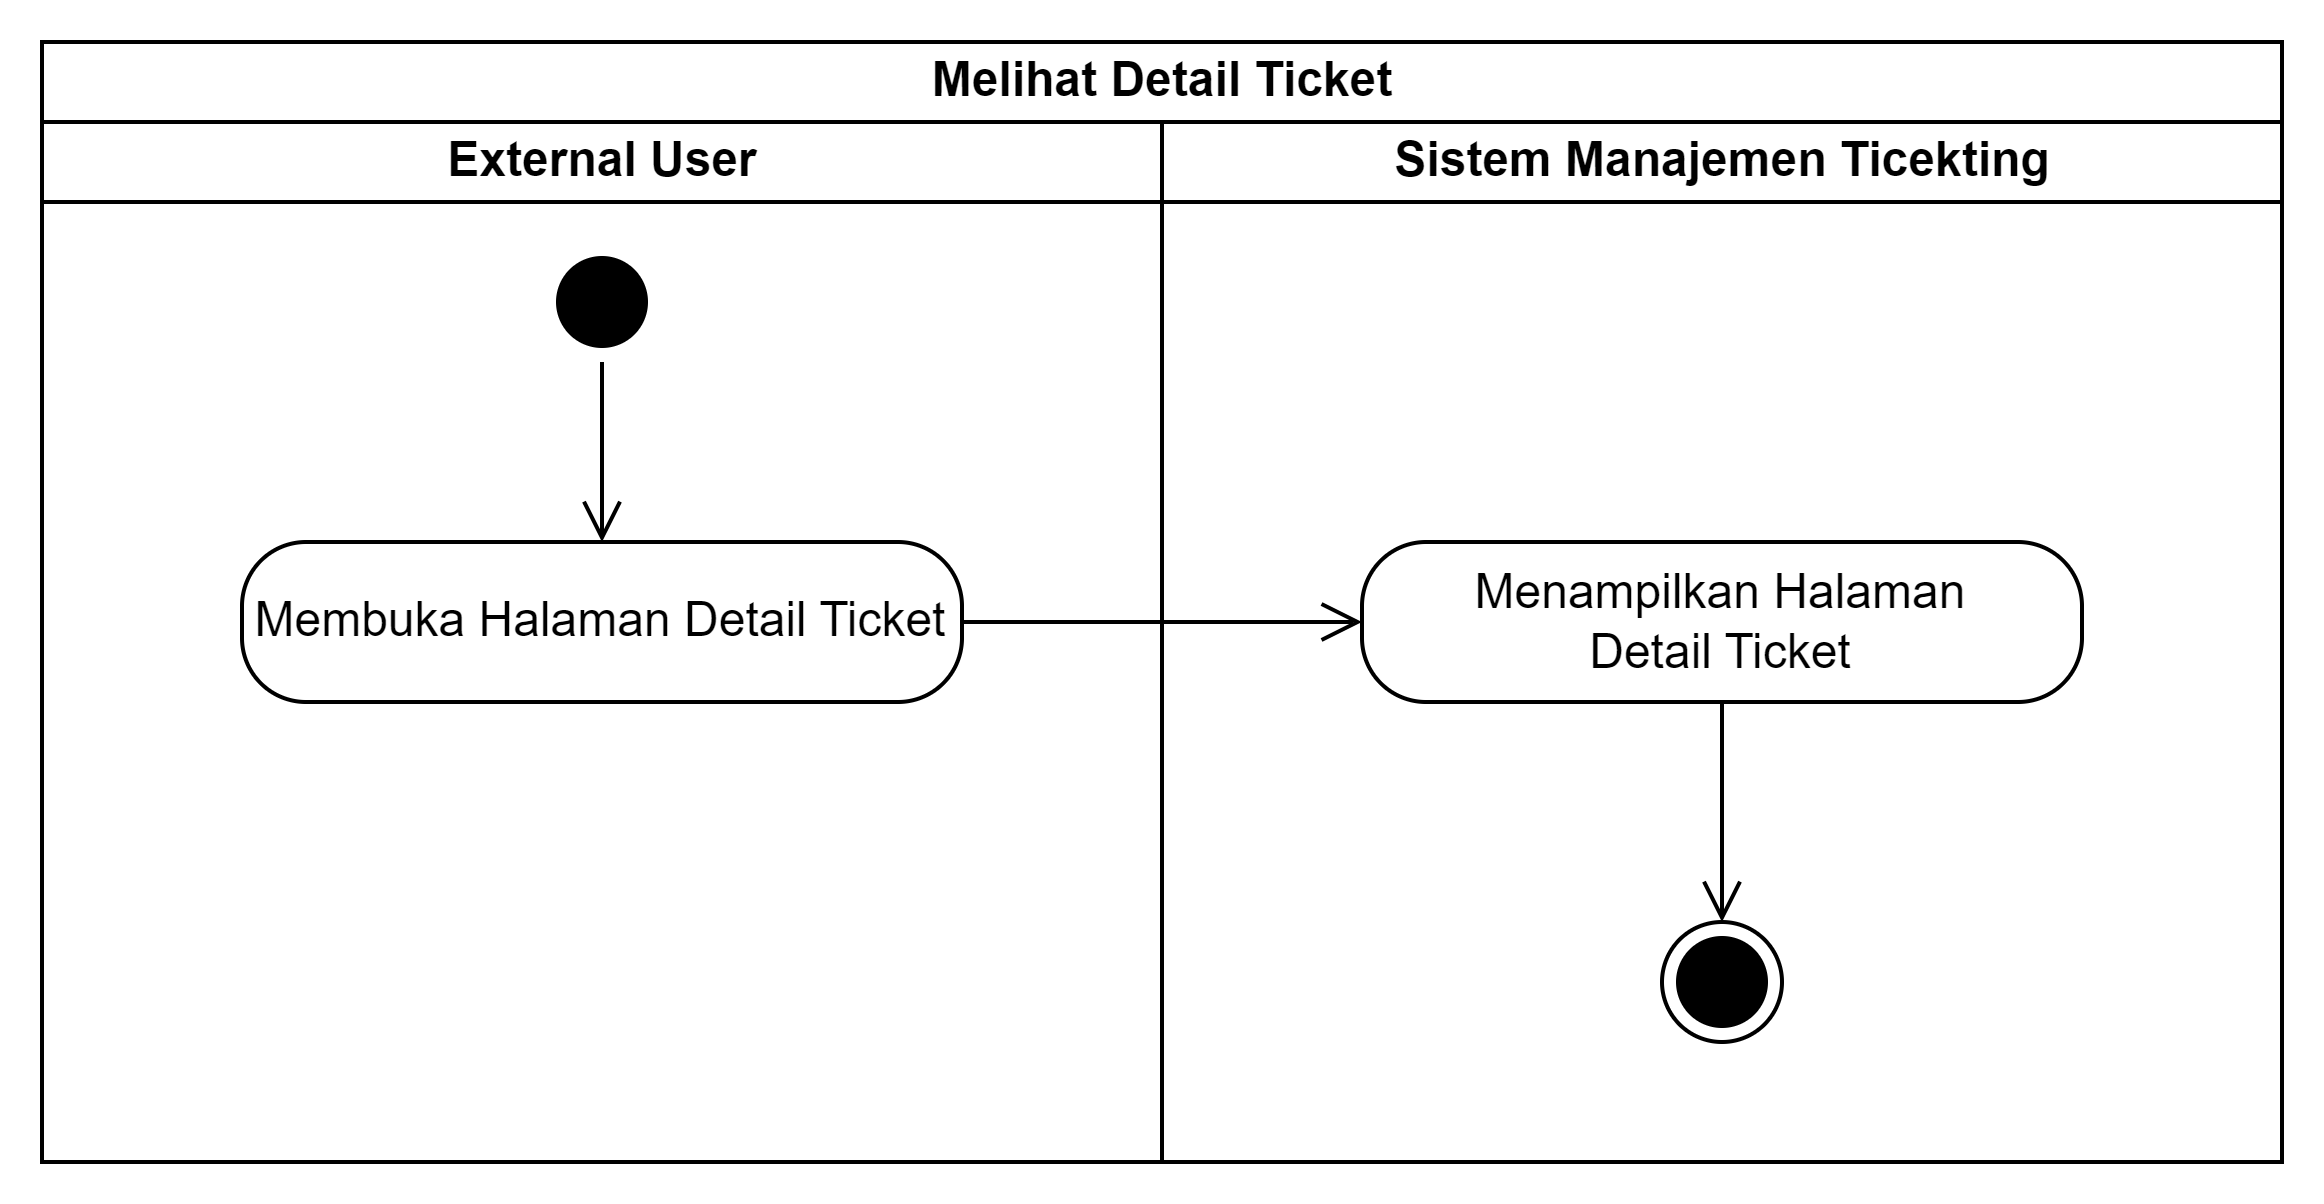
\includegraphics[width=0.75\textwidth]{images/activity/ex/Melihat Detail Ticket.png}
                    \caption{Activity Diagram Melihat Detail Ticket (External User)}
                    \label{fig:AD-PIC-04}
                \end{figure}

                \item Activity Diagram Menutup Ticket

                \hspace*{10pt}
                \begin{tabularx}{.9\linewidth}{@{} l l X @{}}
                    ID Activity & : & AD-PIC-05 \\

                    Deskripsi &	: & Activity Diagram berikut merupakan sebuah proses aktivitas yang dilakukan untuk menutup ticket yang telah dibuat oleh seorang external user dan dikerjakan internal user yang ditunjukkan pada gambar \ref{fig:AD-PIC-05}.
                \end{tabularx}

                \begin{figure}[H]
                    \centering 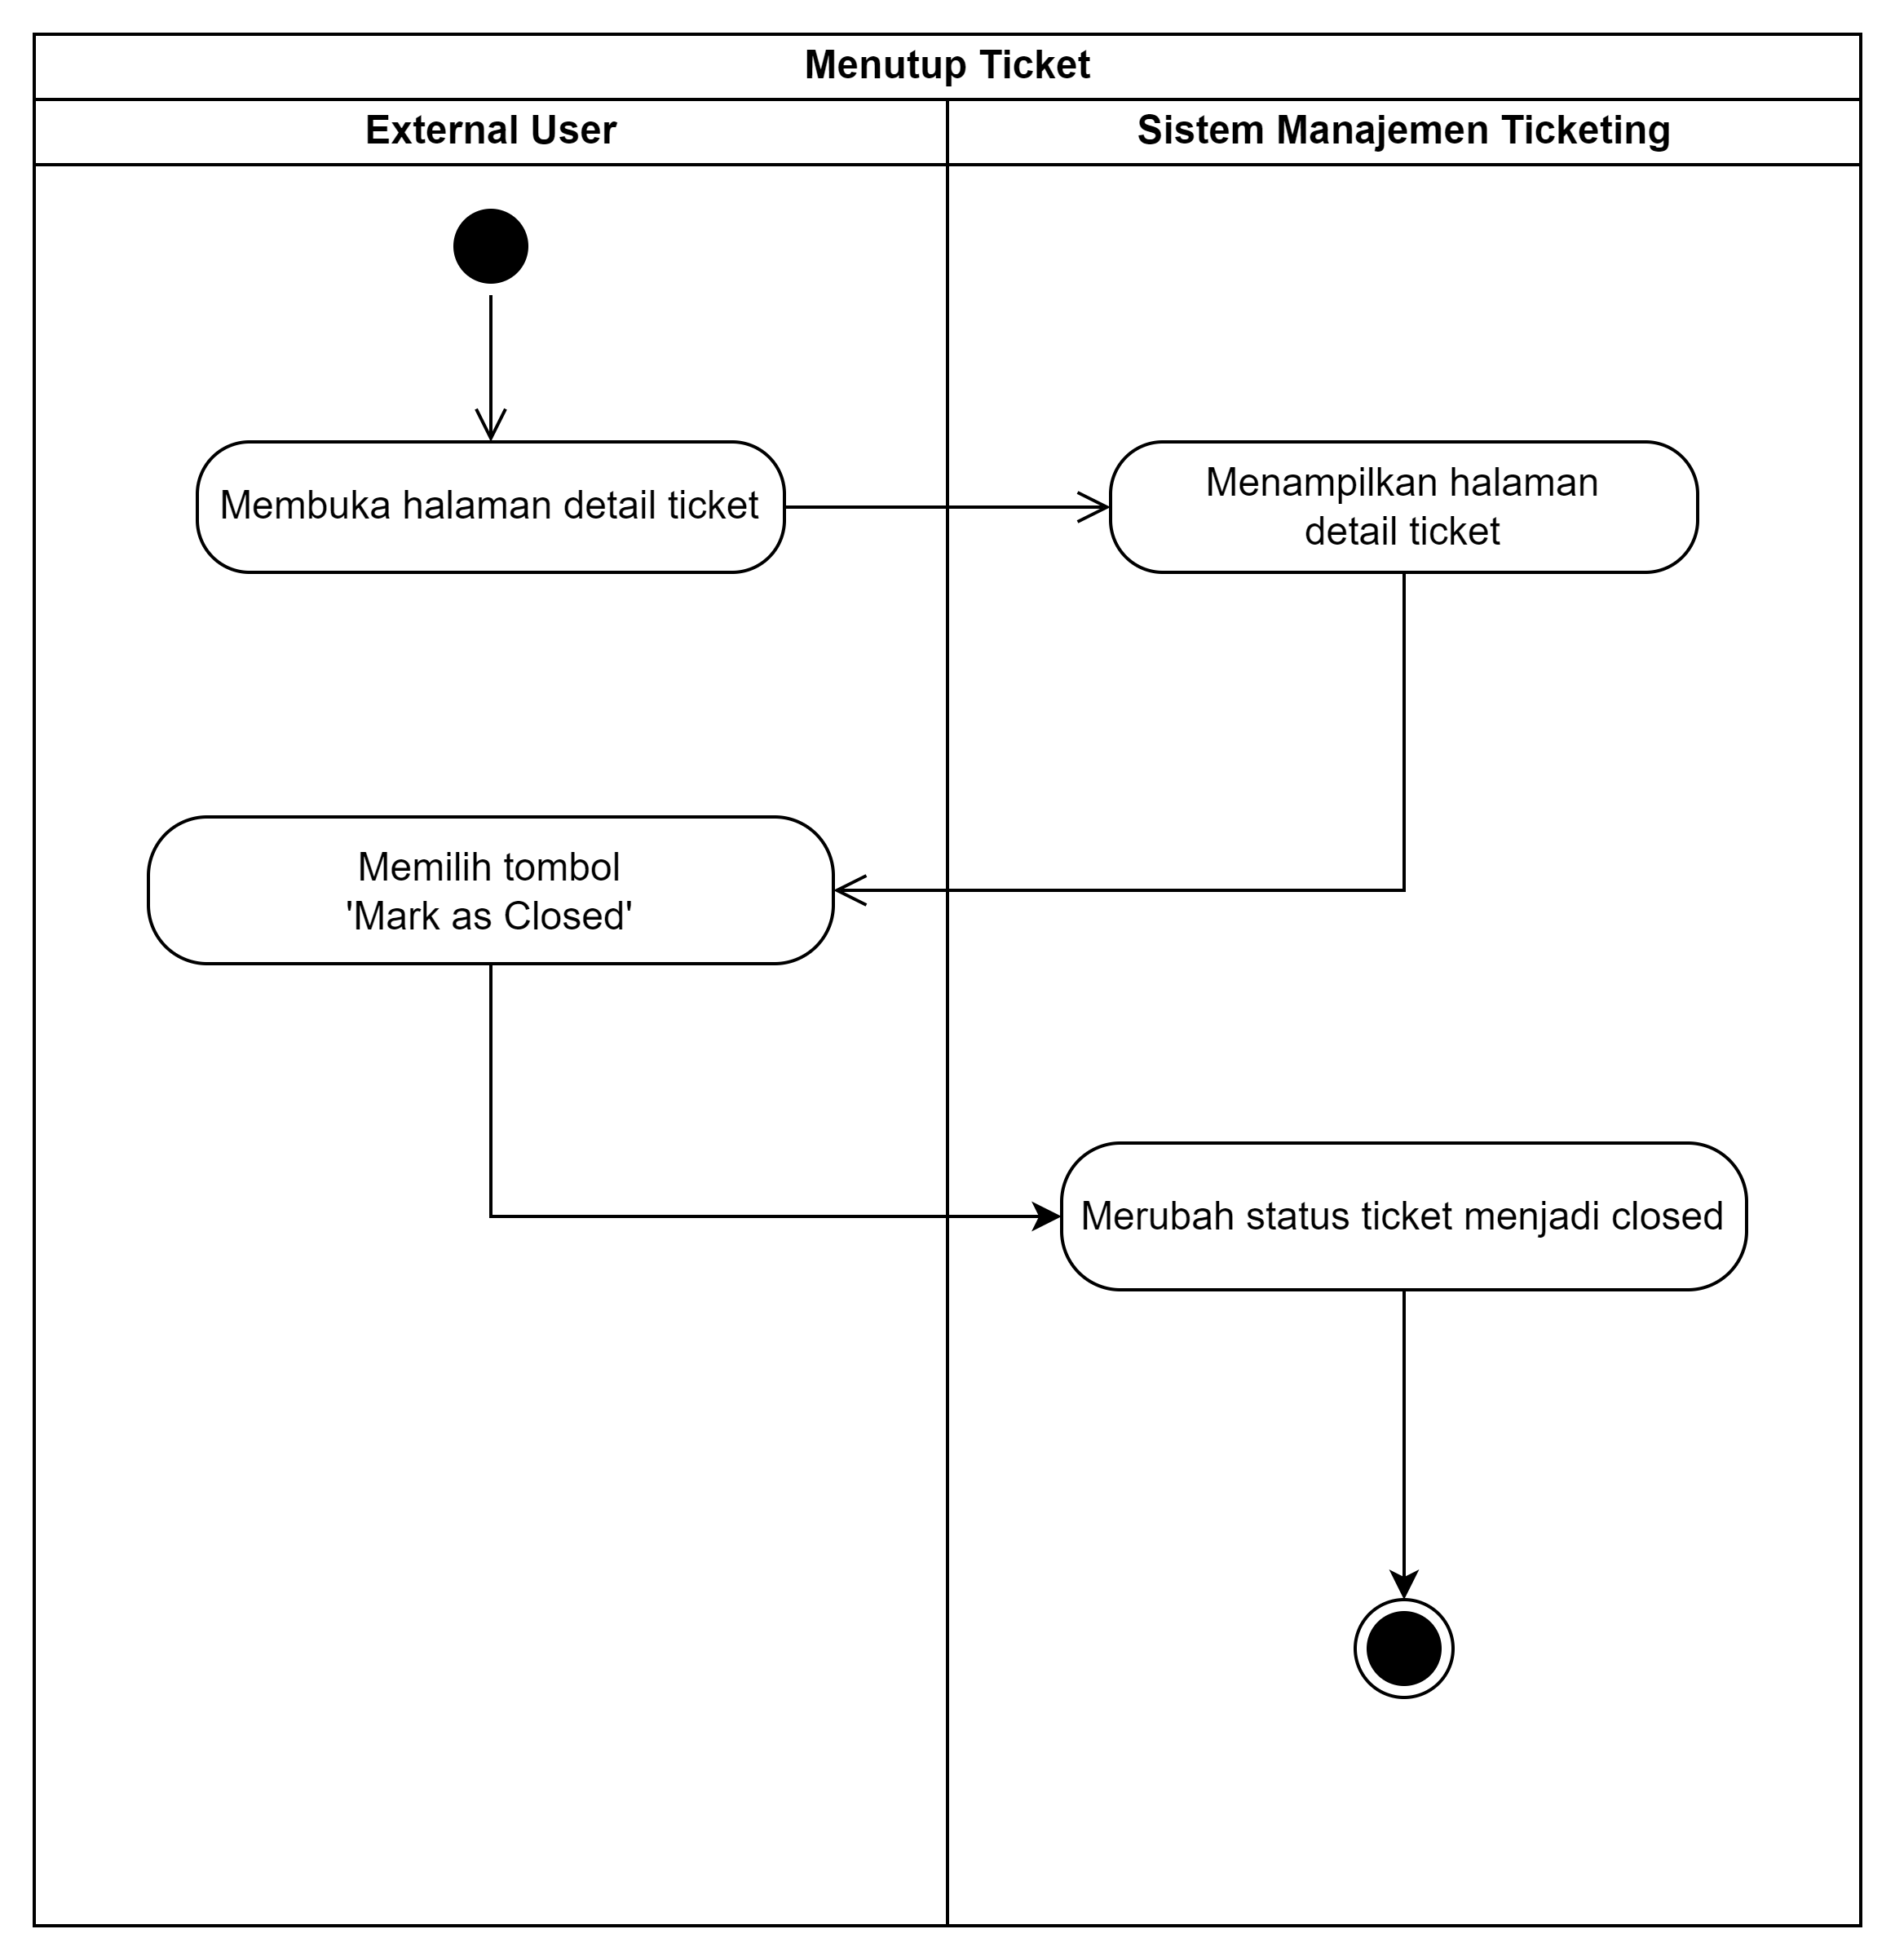
\includegraphics[width=0.75\textwidth]{images/activity/ex/Menutup Ticket.png}
                    \caption{Activity Diagram Menutup Ticket (External User)}
                    \label{fig:AD-PIC-05}
                \end{figure}

                \item Activity Diagram Merevisi Ticket

                \hspace*{10pt}
                \begin{tabularx}{.9\linewidth}{@{} l l X @{}}
                    ID Activity & : & AD-PIC-06 \\

                    Deskripsi &	: & Activity Diagram berikut merupakan sebuah proses aktivitas yang dilakukan untuk merevisi ticket yang telah dibuat oleh seorang external user dan dikerjakan internal user yang ditunjukkan pada gambar \ref{fig:AD-PIC-06}.
                \end{tabularx}

                \begin{figure}[H]
                    \centering 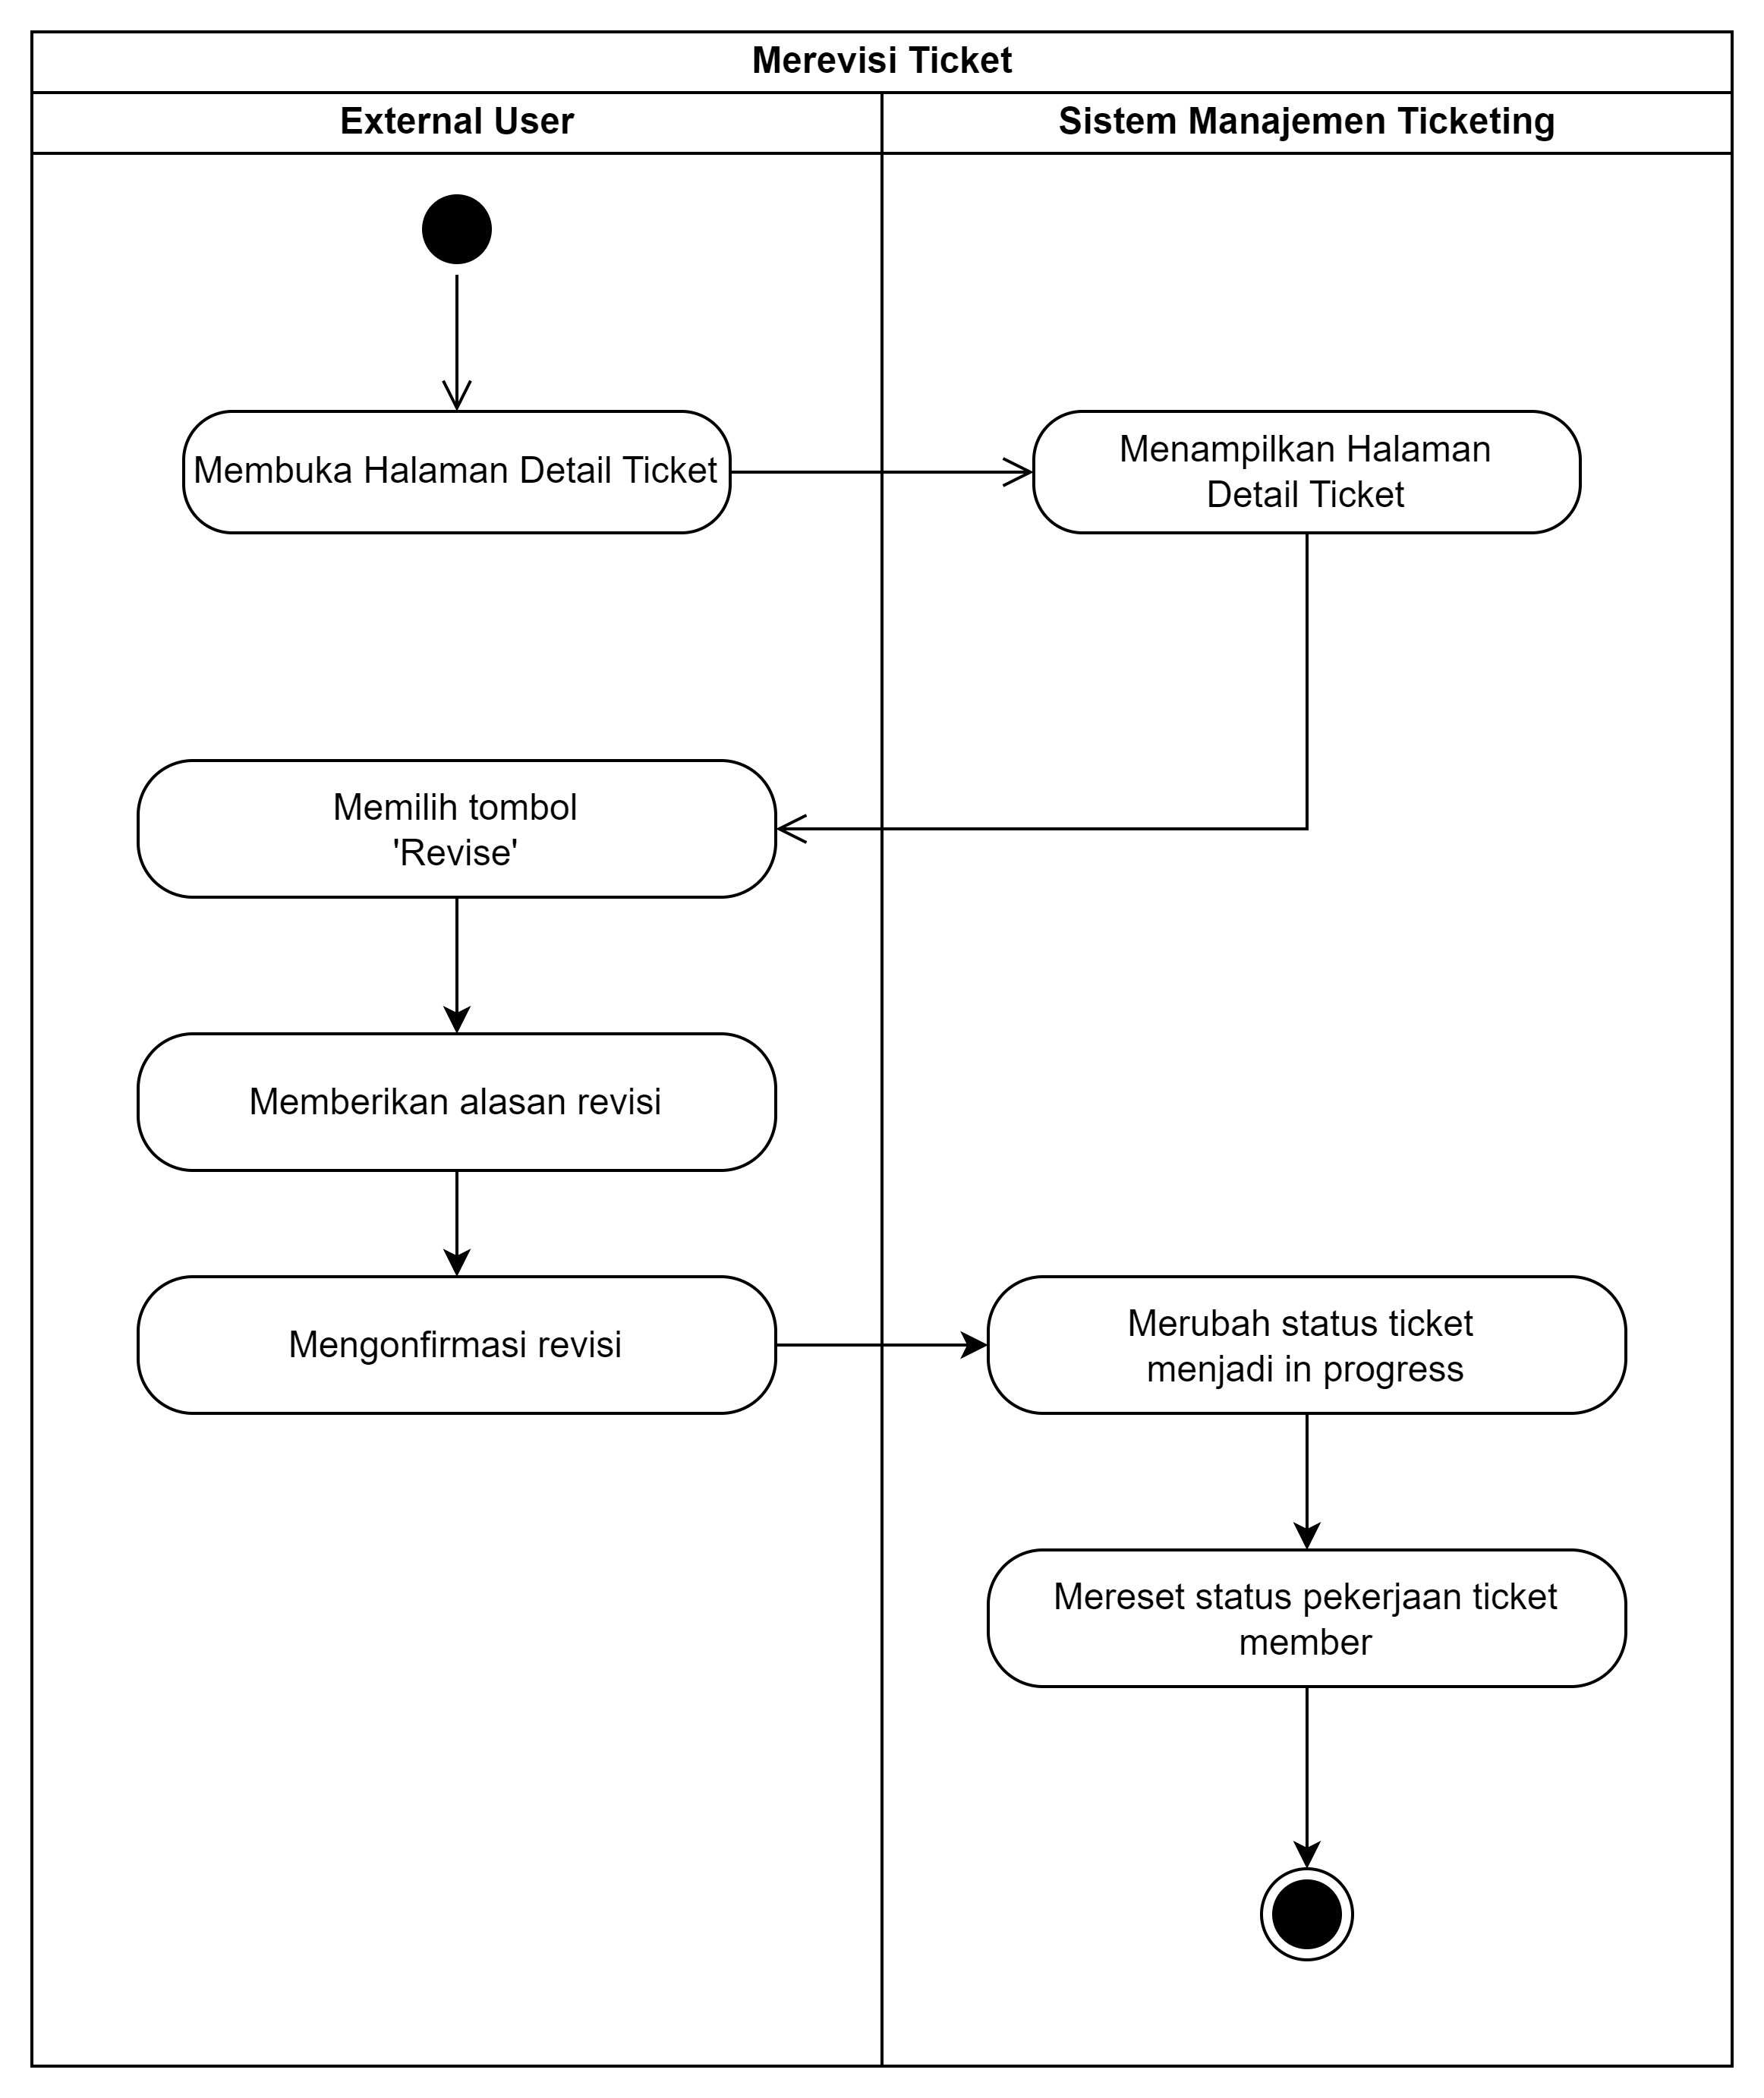
\includegraphics[width=0.75\textwidth]{images/activity/ex/Merevisi Ticket.png}
                    \caption{Activity Diagram Merevisi Ticket (External User)}
                    \label{fig:AD-PIC-06}
                \end{figure}

                \item Activity Diagram Berkomunikasi dengan Product Manager

                \hspace*{10pt}
                \begin{tabularx}{.9\linewidth}{@{} l l X @{}}
                    ID Activity & : & AD-PIC-07 \\
                
                    Deskripsi &	: & Activity Diagram berikut merupakan sebuah proses aktivitas yang dilakukan untuk berkomunikasi dengan Product Manager oleh seorang external user yang ditunjukkan pada gambar \ref{fig:AD-PIC-07}.
                \end{tabularx}

                \begin{figure}[H]
                    \centering 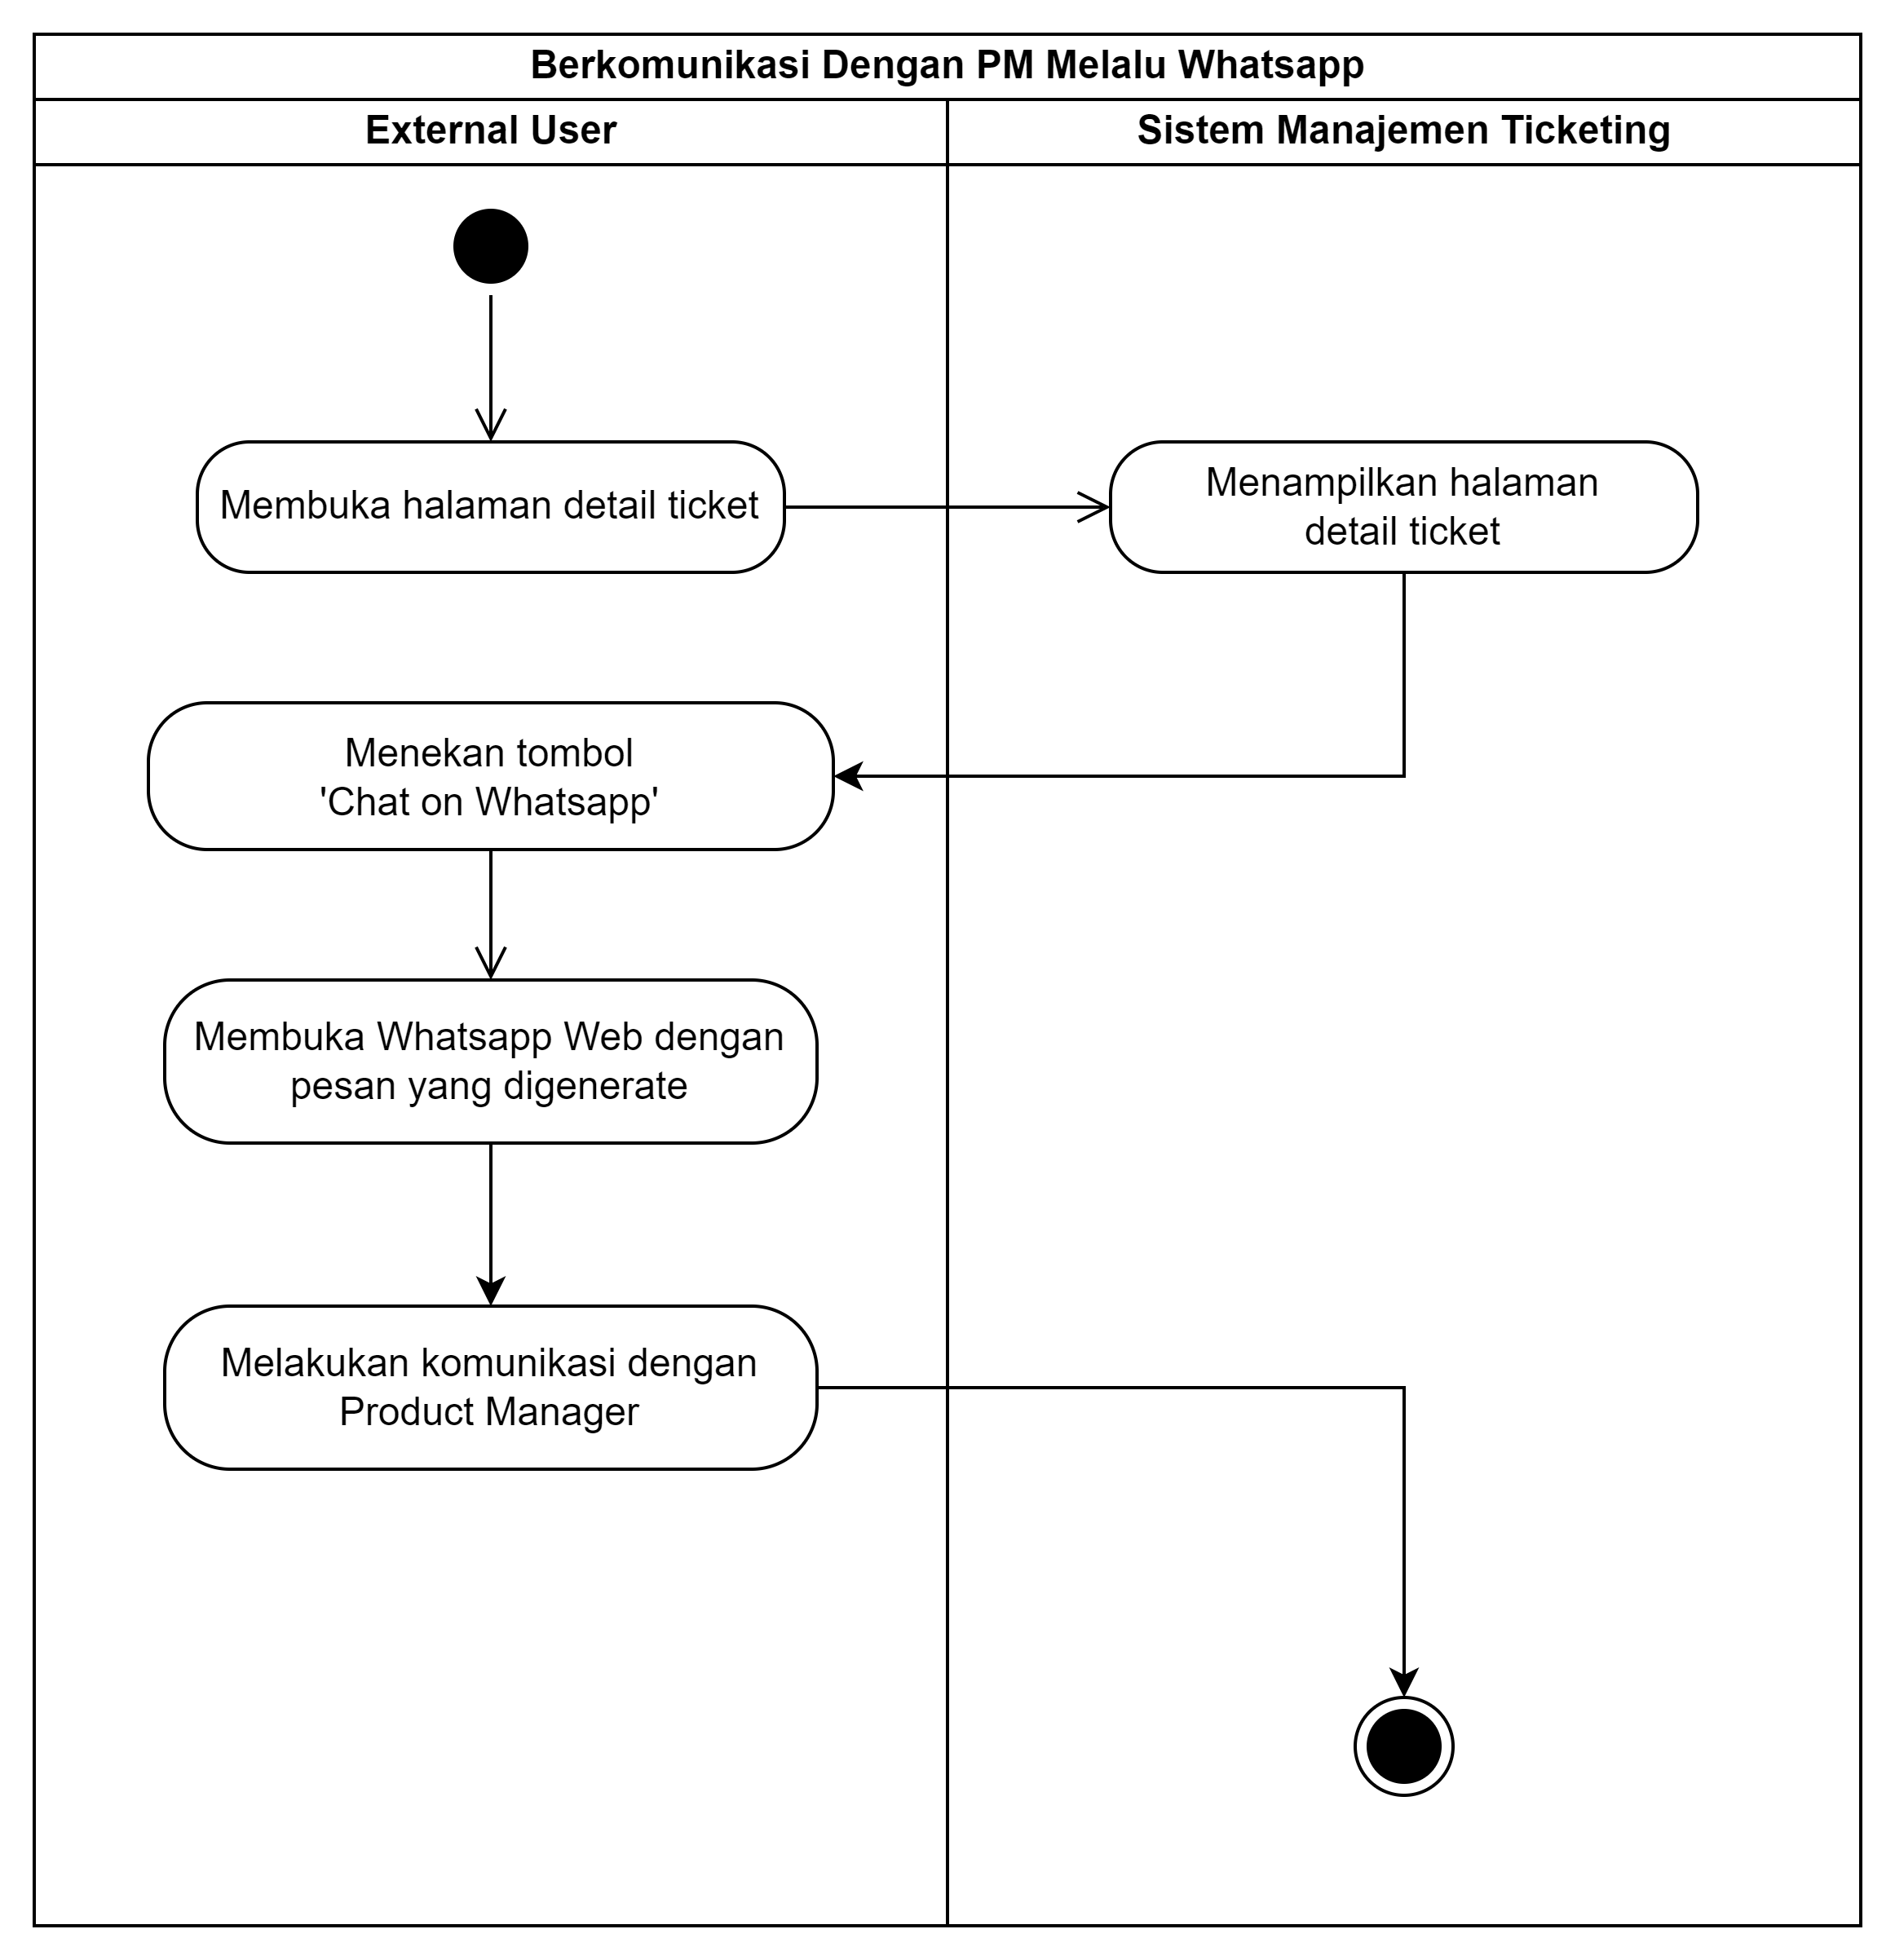
\includegraphics[width=0.75\textwidth]{images/activity/ex/berkomunikasi dengan PM melalui Whatsapp.png}
                    \caption{Activity Diagram Berkomunikasi Dengan PM Melalui Whatsapp (External User)}
                    \label{fig:AD-PIC-07}
                \end{figure}
            \end{enumerate}
        \end{enumerate}
        
        \newpage

        \listsection{Sequence Diagram}

        Berdasarkan activity diagram yang telah dibuat, berikut adalah sequence diagram untuk Sistem Informasi Manajemen Produk dan Ticketing bagian ticketing di PT. Teknologi Aplikasi Sejahtera

        \begin{enumerate}[label=\textbf{4.2.2.\arabic*.}, wide, labelwidth=!, labelindent=0pt]
            \listsection{Sequence Diagram Internal User (Product Manager)}
            
            \begin{enumerate}[label=\arabic*.]
                
                \item Sequence Diagram Melihat List Ticket
                
                % \hspace*{10pt}
                \begin{tabularx}{.9\linewidth}{@{} l l X @{}}
                    ID Sequence & : & SQ-PM-01 \\
                    Deskripsi &	: & Sequence Diagram yang ditunjukkan pada gambar \ref{fig:SQ-PM-01} merupakan sebuah proses aktivitas yang dilakukan untuk melihat list ticket oleh seorang internal user dengan role product manager. 
        
                \end{tabularx}

                % \hspace*{10pt}
                \noindent
                Berikut merupakan class class yang ada pada sequence diagram yang ditunjukkan pada gambar \ref{fig:SQ-PM-01}:

                \begin{tabularx}{.9\linewidth}{@{} l l X @{}}
                    Class Boundary &	: &  TicketPage \\
                    Class Control &	: &  TicketController \\
                    Class Entity &	: &  User, Employee, Ticket, Ticket Member, Product Member, Ticket Category, Ticket Status, dan Ticket Priority

                \end{tabularx}
            
                
                \item Sequence Diagram Memfilter List Ticket
                
                \begin{tabularx}{.9\linewidth}{@{} l l X @{}}
                    ID Sequence &	: & SQ-PM-02 \\
                    Deskripsi &	: & Sequence Diagram berikut merupakan sebuah proses aktivitas yang dilakukan untuk memfilter ticket oleh seorang internal user dengan role product manager. 
        
                \end{tabularx}

                \noindent Berikut merupakan class class yang ada pada sequence diagram yang ditunjukkan pada gambar 4.22:

                \begin{tabularx}{.9\linewidth}{@{} l l X @{}}
                    Class Boundary & : & TicketPage \\
                    Class Control & : & TicketController \\
                    Class Entity & : &  User, Employee, Ticket, Ticket Member, Product Member, Ticket Category, Ticket Status, Ticket Priority
                    
                \end{tabularx}

                
                \item Sequence Diagram Melihat Detail Ticket
                
                \begin{tabularx}{.9\linewidth}{@{} l l X @{}}
                    ID Sequence &	: & SQ-PM-03 \\
                    Deskripsi &	: & Sequence Diagram berikut merupakan sebuah proses aktivitas yang dilakukan untuk melihat detail ticket oleh seorang internal user dengan role product manager. 
        
                \end{tabularx}

                \noindent Berikut merupakan class class yang ada pada sequence diagram yang ditunjukkan pada gambar 4.23:

                \begin{tabularx}{.9\linewidth}{@{} l l X @{}}
                    Class Boundary & : & TicketPage \\
                    Class Control & : & TicketController \\
                    Class Entity & : & Ticket
                
                \end{tabularx}
                
                \item Sequence Diagram Memverifikasi List Ticket
                
                \begin{tabularx}{.9\linewidth}{@{} l l X @{}}
                    ID Sequence &	: & SQ-PM-04 \\
                    Deskripsi &	: & Sequence Diagram berikut merupakan sebuah proses aktivitas yang dilakukan untuk memverifikasi ticket yang dibuat external user oleh seorang internal user dengan role product manager. 
        
                \end{tabularx}

                \noindent Berikut merupakan class class yang ada pada sequence diagram yang ditunjukkan pada gambar 4.24:

                \begin{tabularx}{.9\linewidth}{@{} l l X @{}}
                    Class Boundary & : & TicketPage \\
                    Class Control & : & TicketController \\
                    Class Entity & : & Ticket
                
                \end{tabularx}
                
                \item Sequence Diagram Menolak Ticket
                
                \begin{tabularx}{.9\linewidth}{@{} l l X @{}}
                    ID Sequence &	: & SQ-PM-05 \\
                    Deskripsi &	: & Sequence Diagram berikut merupakan sebuah proses aktivitas yang dilakukan untuk menolak ticket yang dibuat external user oleh seorang internal user dengan role product manager. 
        
                \end{tabularx}

                \noindent Berikut merupakan class class yang ada pada sequence diagram yang ditunjukkan pada gambar 4.25:

                \begin{tabularx}{.9\linewidth}{@{} l l X @{}}
                    Class Boundary & : & TicketPage \\
                    Class Control & : & TicketController \\
                    Class Entity & : & Ticket, ProductMember, TicketMember  
                
                \end{tabularx}

                \item Sequence Diagram Merevisi Ticket
                
                \begin{tabularx}{.9\linewidth}{@{} l l X @{}}
                    ID Sequence &	: & SQ-PM-06 \\
                    Deskripsi &	: & Sequence Diagram berikut merupakan sebuah proses aktivitas yang dilakukan untuk merevisi ticket yang telah dikerjakan developer oleh seorang internal user dengan role product manager. 
        
                \end{tabularx}

                \noindent Berikut merupakan class class yang ada pada sequence diagram yang ditunjukkan pada gambar 4.26:

                \begin{tabularx}{.9\linewidth}{@{} l l X @{}}
                    Class Boundary & : & TicketPage \\
                    Class Control & : & TicketController \\
                    Class Entity & : & Ticket
                
                \end{tabularx}
            
                
                \item Sequence Diagram Berkomunikasi dengan external user
                
                \begin{tabularx}{.9\linewidth}{@{} l l X @{}}
                    ID Sequence &	: & SQ-PM-07 \\
                    Deskripsi &	: & Sequence Diagram berikut merupakan sebuah proses aktivitas yang dilakukan untuk berkomunikasi dengan external user oleh seorang internal user dengan role product manager. 
        
                \end{tabularx}

                \noindent Berikut merupakan class class yang ada pada sequence diagram yang ditunjukkan pada gambar 4.27:

                \begin{tabularx}{.9\linewidth}{@{} l l X @{}}
                    Class Boundary & : & TicketPage \\
                    Class Control & : & TicketController \\
                    Class Entity & : & Ticket
                
                \end{tabularx}


                \item Sequence Diagram Mengubah Status Ticket Menjadi Done
                
                \begin{tabularx}{.9\linewidth}{@{} l l X @{}}
                    ID Sequence &	: & SQ-PM-08 \\
                    Deskripsi &	: & Sequence Diagram berikut merupakan sebuah proses aktivitas yang dilakukan untuk mengubah status ticket menjadi done oleh internal user dengan role product manager. 
        
                \end{tabularx}

                \noindent Berikut merupakan class class yang ada pada sequence diagram yang ditunjukkan pada gambar 4.28:

                \begin{tabularx}{.9\linewidth}{@{} l l X @{}}
                    Class Boundary & : & TicketPage \\
                    Class Control & : & TicketController \\
                    Class Entity & : & Ticket
                
                \end{tabularx}
            
                
                \begin{sidewaysfigure}
                    \centering 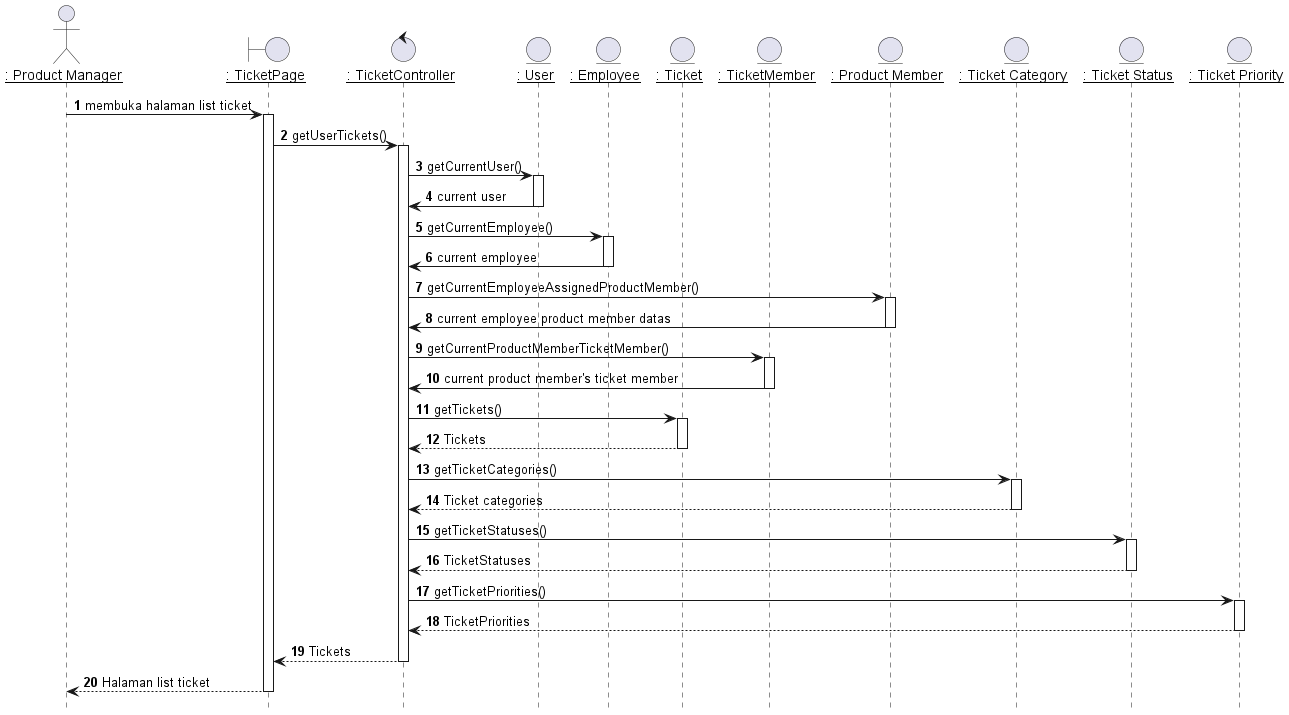
\includegraphics[width=\textwidth]{out/plantuml/sequence/ipm/ipm1/Melihat List Ticket.png}
                    \caption{Sequence Diagram Melihat List Ticket (PM)}
                    \label{fig:SQ-PM-01}
                \end{sidewaysfigure}

                \begin{sidewaysfigure}
                    \centering 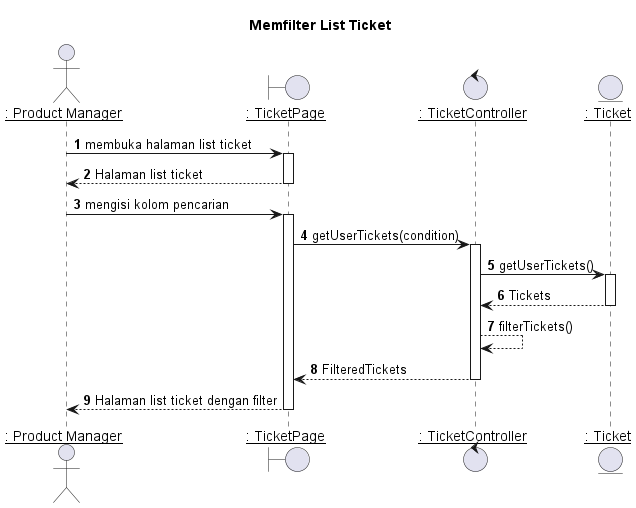
\includegraphics[width=\textwidth]{out/plantuml/sequence/ipm/ipm2/Memfilter List Ticket.png}
                    \caption{Sequence Diagram Memfilter List Ticket (PM)}
                    \label{fig:SQ-PM-02}
                \end{sidewaysfigure}

                \begin{sidewaysfigure}
                    \centering 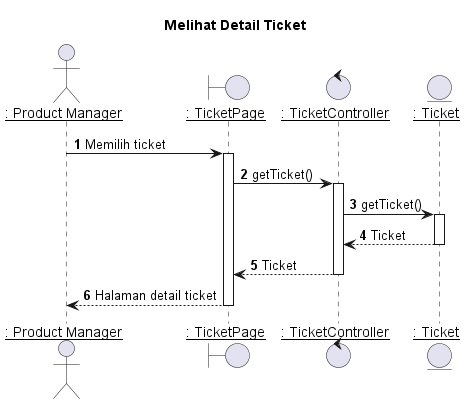
\includegraphics[width=\textwidth]{out/plantuml/sequence/ipm/ipm3/Melihat Detail Ticket.png}
                    \caption{Sequence Diagram Melihat Detail Ticket (PM)}
                    \label{fig:SQ-PM-03}
                \end{sidewaysfigure}

                \begin{sidewaysfigure}
                    \centering 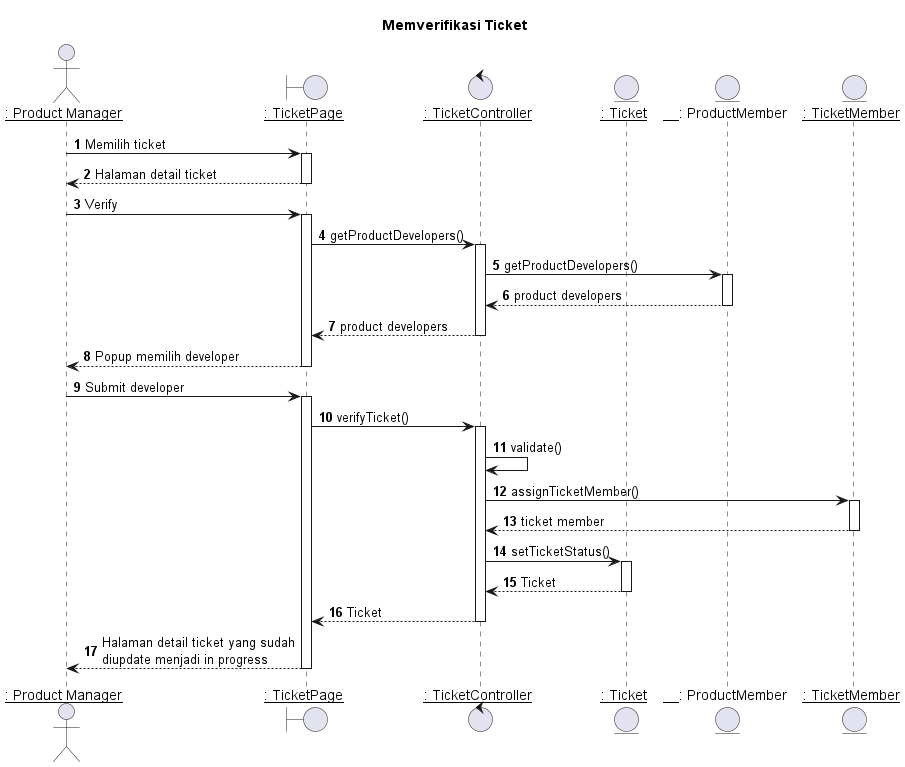
\includegraphics[width=\textwidth]{out/plantuml/sequence/ipm/ipm4/Memverifikasi Ticket.png}
                    \caption{Sequence Diagram Memverifikasi Ticket (PM)}
                    \label{fig:SQ-PM-04}
                \end{sidewaysfigure}

                \begin{sidewaysfigure}
                    \centering 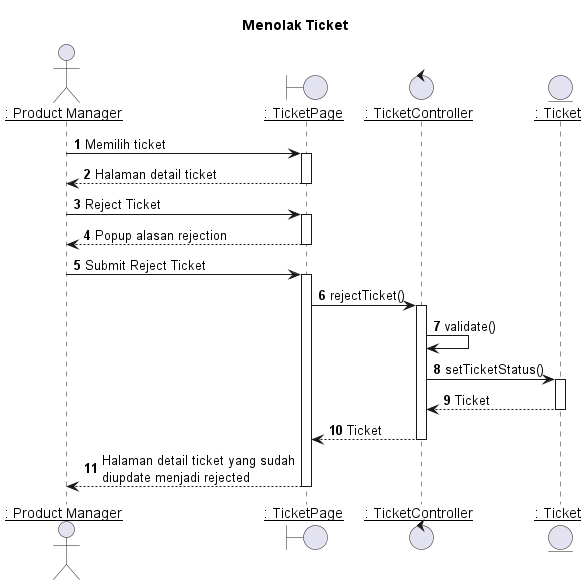
\includegraphics[width=\textwidth]{out/plantuml/sequence/ipm/ipm5/Menolak Ticket.png}
                    \caption{Sequence Diagram Menolak Ticket (PM)}
                    \label{fig:SQ-PM-05}
                \end{sidewaysfigure}

                \begin{sidewaysfigure}
                    \centering 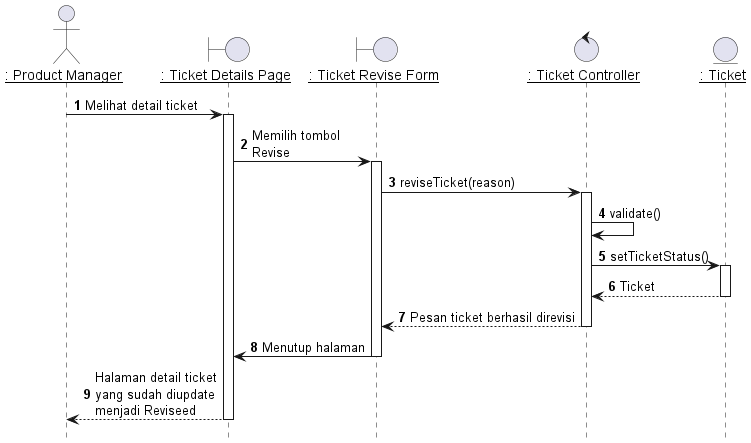
\includegraphics[width=\textwidth]{out/plantuml/sequence/ipm/ipm6/Merevisi Ticket.png}
                    \caption{Sequence Diagram Merevisi Ticket (PM)}
                    \label{fig:SQ-PM-06}
                \end{sidewaysfigure}

                \begin{sidewaysfigure}
                    \centering 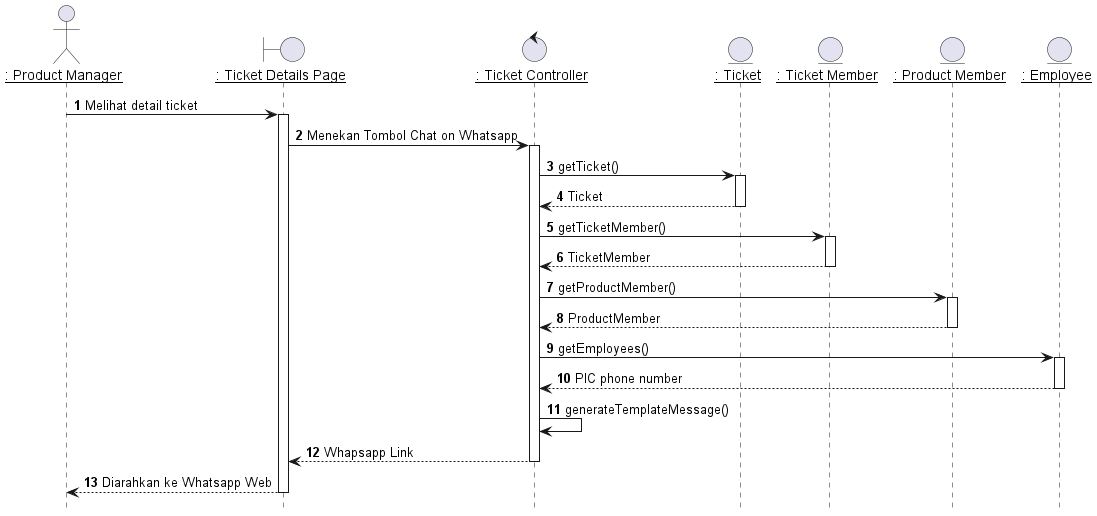
\includegraphics[width=\textwidth]{out/plantuml/sequence/ipm/ipm7/Berkomunikasi Dengan PIC Melalui Whatsapp.png}
                    \caption{Sequence Diagram Berkomunikasi Dengan PM Melalui Whatsapp (PM)}
                    \label{fig:SQ-PM-07}
                \end{sidewaysfigure}

                \begin{sidewaysfigure}
                    \centering 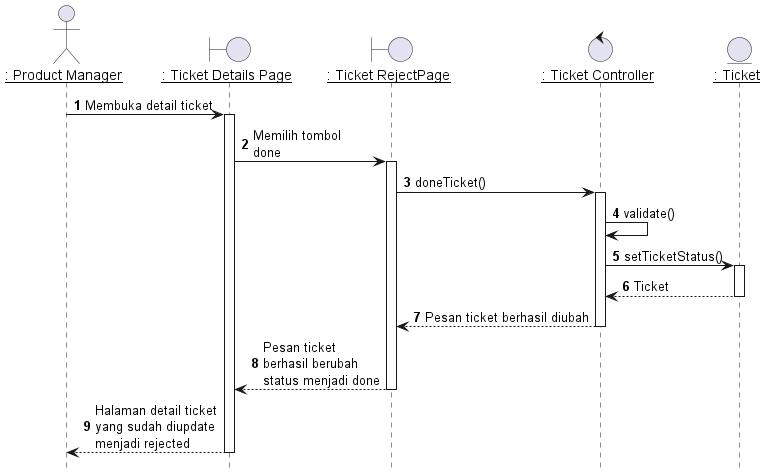
\includegraphics[width=\textwidth]{out/plantuml/sequence/ipm/ipm8/Mengubah Status Ticket Menjadi Done.png}
                    \caption{Sequence Diagram Mengubah Status Ticket Menjadi Done (PM)}
                    \label{fig:SQ-PM-08}
                \end{sidewaysfigure}
            \end{enumerate}

            \newpage
            \listsection{Sequence Diagram Internal User (Developer)}
            
            \begin{enumerate}[label=\arabic*.]
                \item Sequence Diagram Melihat List Ticket
                
                \begin{tabularx}{.9\linewidth}{@{} l l X @{}}
                    ID Sequence &	: & SQ-DEV-01 \\
                    Deskripsi &	: & Sequence Diagram berikut merupakan sebuah proses aktivitas yang dilakukan untuk melihat list ticket oleh internal user dengan role developer. 
        
                \end{tabularx}

                \noindent Berikut merupakan class class yang ada pada sequence diagram yang ditunjukkan pada gambar 4.29:

                \begin{tabularx}{.9\linewidth}{@{} l l X @{}}
                    Class Boundary & : & TicketPage \\
                    Class Control & : & TicketController \\
                    Class Entity & : & Ticket
                
                \end{tabularx}
                
                \item Sequence Diagram Memfilter Ticket
                
                \begin{tabularx}{.9\linewidth}{@{} l l X @{}}
                    ID Sequence &	: & SQ-DEV-02 \\
                    Deskripsi &	: & Sequence Diagram berikut merupakan sebuah proses aktivitas yang dilakukan untuk memfilter list ticket oleh internal user dengan role developer. 
        
                \end{tabularx}

                \noindent Berikut merupakan class class yang ada pada sequence diagram yang ditunjukkan pada gambar 4.30:

                \begin{tabularx}{.9\linewidth}{@{} l l X @{}}
                    Class Boundary & : & TicketPage \\
                    Class Control & : & TicketController \\
                    Class Entity & : & Ticket
                
                \end{tabularx}
                
                \item Sequence Diagram Melihat Detail Ticket
                
                \begin{tabularx}{.9\linewidth}{@{} l l X @{}}
                    ID Sequence &	: & SQ-DEV-03 \\
                    Deskripsi &	: & Sequence Diagram berikut merupakan sebuah proses aktivitas yang dilakukan untuk melihat detail ticket oleh internal user dengan role developer. 
        
                \end{tabularx}

                \noindent Berikut merupakan class class yang ada pada sequence diagram yang ditunjukkan pada gambar 4.31:

                \begin{tabularx}{.9\linewidth}{@{} l l X @{}}
                    Class Boundary & : & TicketPage \\
                    Class Control & : & TicketController \\
                    Class Entity & : & Ticket
                
                \end{tabularx}
                
                \item Sequence Diagram Melaporkan Pengerjaan Ticket
                
                \begin{tabularx}{.9\linewidth}{@{} l l X @{}}
                    ID Sequence &	: & SQ-DEV-04 \\
                    Deskripsi &	: & Sequence Diagram berikut merupakan sebuah proses aktivitas yang dilakukan untuk melaporkan pengerjaan ticket oleh internal user dengan role developer. 
        
                \end{tabularx}

                \noindent Berikut merupakan class class yang ada pada sequence diagram yang ditunjukkan pada gambar 4.32:

                \begin{tabularx}{.9\linewidth}{@{} l l X @{}}
                    Class Boundary & : & TicketPage \\
                    Class Control & : & TicketController \\
                    Class Entity & : & Ticket
                
                \end{tabularx}


                
                
                \begin{sidewaysfigure}
                    \centering 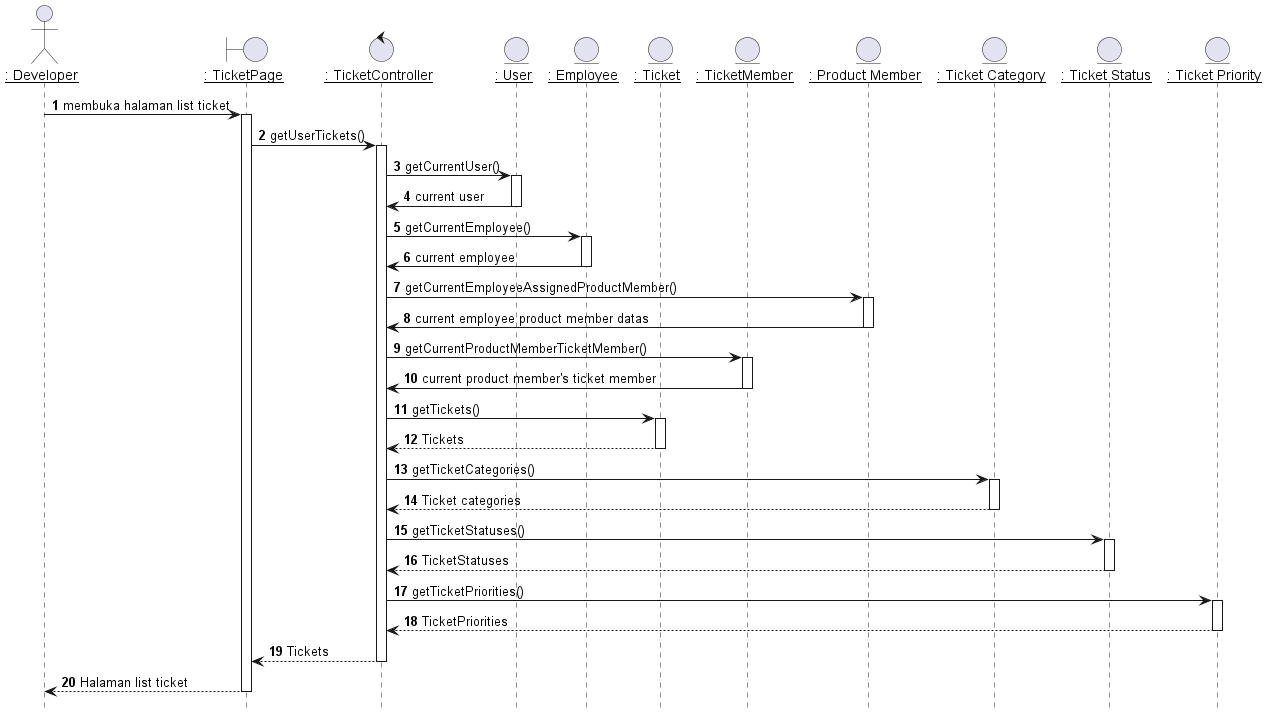
\includegraphics[width=\textwidth]{out/plantuml/sequence/idev/idev1/Melihat List Ticket.png}
                    \caption{Sequence Diagram Melihat List Ticket (DEV)}
                    \label{fig:SQ-DEV-01}
                \end{sidewaysfigure}

                \begin{sidewaysfigure}
                    \centering 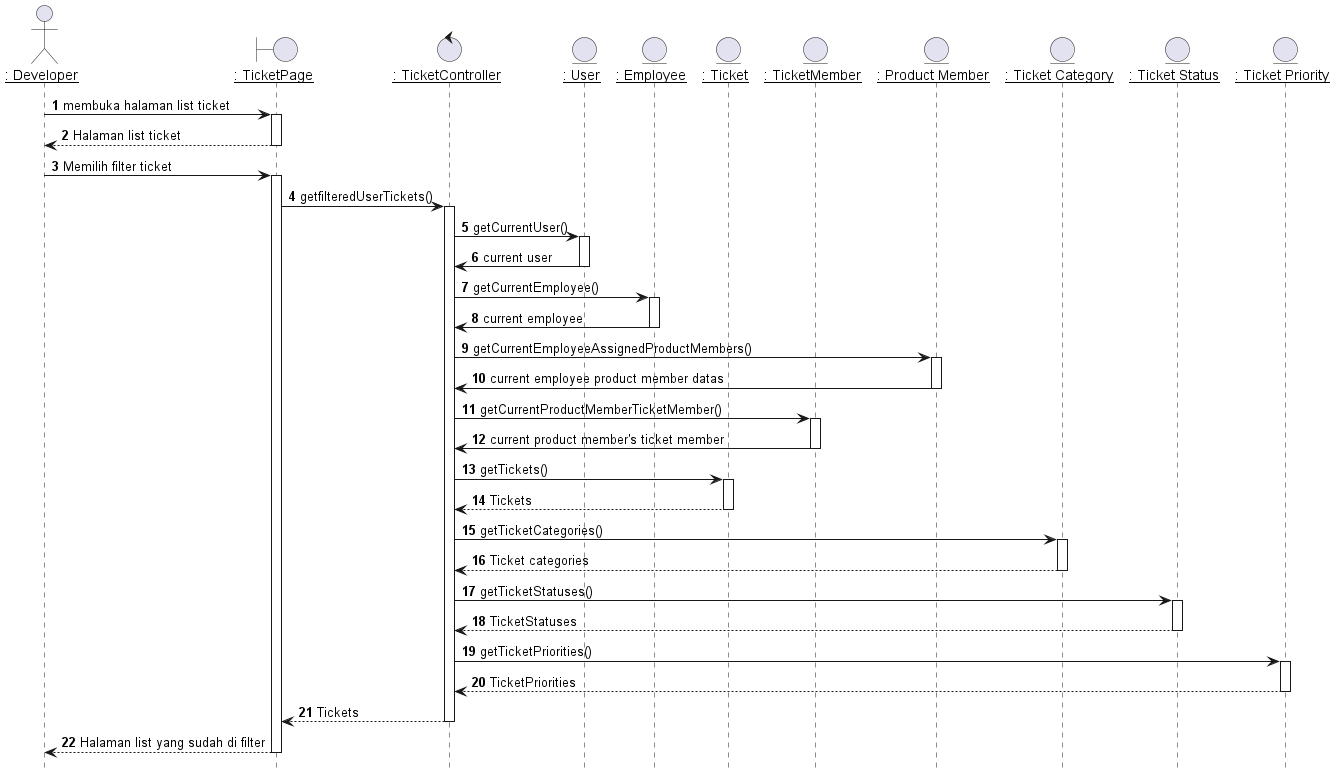
\includegraphics[width=\textwidth]{out/plantuml/sequence/idev/idev2/Memfilter List Ticket.png}
                    \caption{Sequence Diagram Memfilter List Ticket (DEV)}
                    \label{fig:SQ-DEV-02}
                \end{sidewaysfigure}

                \begin{sidewaysfigure}
                    \centering 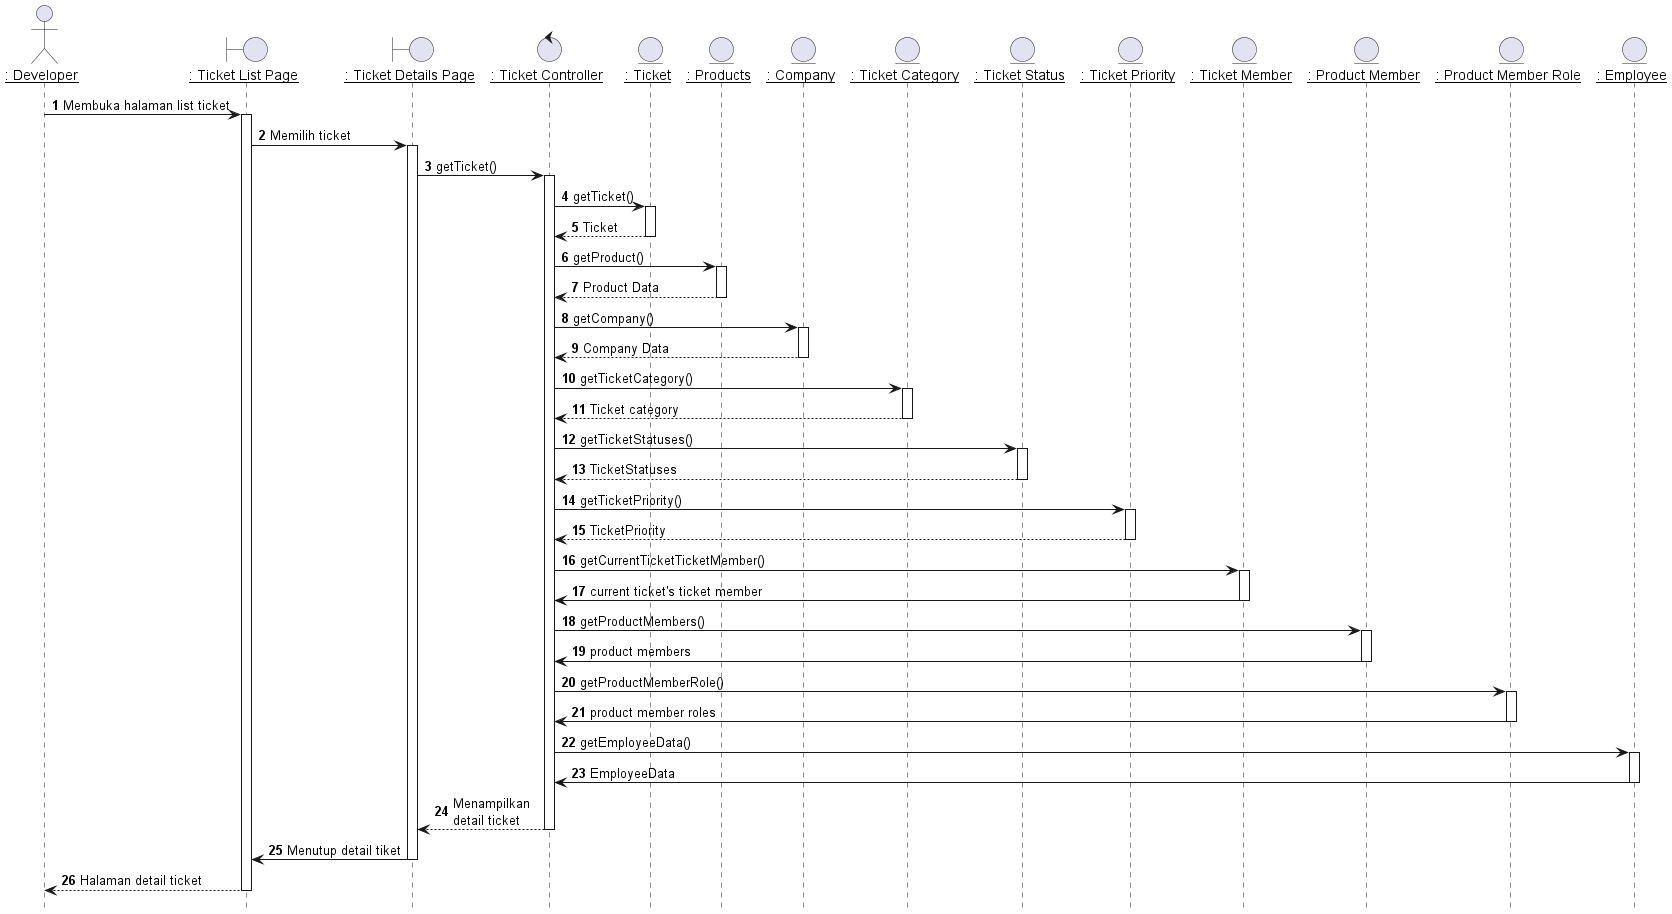
\includegraphics[width=\textwidth]{out/plantuml/sequence/idev/idev3/Melihat Detail Ticket.png}
                    \caption{Sequence Diagram Melihat Detail Ticket (DEV)}
                    \label{fig:SQ-DEV-03}
                \end{sidewaysfigure}

                \begin{sidewaysfigure}
                    \centering 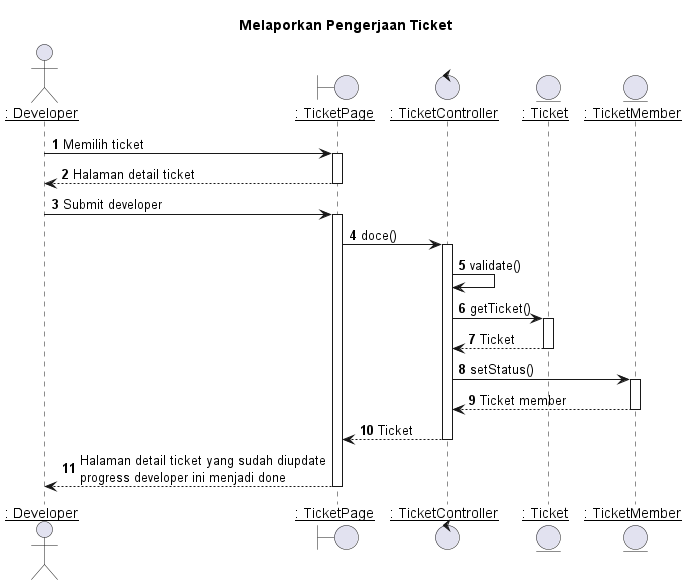
\includegraphics[width=\textwidth]{out/plantuml/sequence/idev/idev4/Melaporkan Pengerjaan Ticket.png}
                    \caption{Sequence Diagram Melaporkan Pengerjaan Ticket (DEV)}
                    \label{fig:SQ-DEV-04}
                \end{sidewaysfigure}
            \end{enumerate}

            \newpage
            \listsection{Sequence Diagram External User}

            \begin{enumerate}[label=\arabic*.]
                \item Sequence Diagram Melihat List Ticket
                
                \begin{tabularx}{.9\linewidth}{@{} l l X @{}}
                    ID Sequence &	: & SQ-PIC-01 \\
                    Deskripsi &	: & Sequence Diagram berikut merupakan sebuah proses aktivitas yang dilakukan untuk melihat list ticket oleh seorang external user. 
        
                \end{tabularx}

                \noindent Berikut merupakan class class yang ada pada sequence diagram yang ditunjukkan pada gambar 4.33:

                \begin{tabularx}{.9\linewidth}{@{} l l X @{}}
                    Class Boundary & : & TicketPage \\
                    Class Control & : & TicketController \\
                    Class Entity & : & Ticket
                
                \end{tabularx}

                \item Sequence Diagram Memfilter List Ticket
                
                \begin{tabularx}{.9\linewidth}{@{} l l X @{}}
                    ID Sequence &	: & SQ-PIC-02 \\
                    Deskripsi &	: & Sequence Diagram berikut merupakan sebuah proses aktivitas yang dilakukan untuk memfilter ticket oleh seorang external user. 
        
                \end{tabularx}

                \noindent Berikut merupakan class class yang ada pada sequence diagram yang ditunjukkan pada gambar 4.34:

                \begin{tabularx}{.9\linewidth}{@{} l l X @{}}
                    Class Boundary & : & TicketPage \\
                    Class Control & : & TicketController \\
                    Class Entity & : & Ticket
                
                \end{tabularx}

                \item Sequence Diagram Membuat Ticket
                
                \begin{tabularx}{.9\linewidth}{@{} l l X @{}}
                    ID Sequence &	: & SQ-PIC-03 \\
                    Deskripsi &	: & Sequence Diagram berikut merupakan sebuah proses aktivitas yang dilakukan untuk membuat ticket oleh seorang external user. 
        
                \end{tabularx}

                \noindent Berikut merupakan class class yang ada pada sequence diagram yang ditunjukkan pada gambar 4.35:

                \begin{tabularx}{.9\linewidth}{@{} l l X @{}}
                    Class Boundary & : & TicketPage \\
                    Class Control & : & TicketController \\
                    Class Entity & : & Ticket
                
                \end{tabularx}
                
                \item Sequence Diagram Melihat Detail Ticket
                
                \begin{tabularx}{.9\linewidth}{@{} l l X @{}}
                    ID Sequence &	: & SQ-PIC-04 \\
                    Deskripsi &	: & Sequence Diagram berikut merupakan sebuah proses aktivitas yang dilakukan untuk melihat detail ticket oleh seorang external user. 
        
                \end{tabularx}

                \noindent Berikut merupakan class class yang ada pada sequence diagram yang ditunjukkan pada gambar 4.36:

                \begin{tabularx}{.9\linewidth}{@{} l l X @{}}
                    Class Boundary & : & TicketPage \\
                    Class Control & : & TicketController \\
                    Class Entity & : & Ticket
                
                \end{tabularx}
                
                \item Sequence Diagram Menutup Ticket
                
                \begin{tabularx}{.9\linewidth}{@{} l l X @{}}
                    ID Sequence &	: & SQ-PIC-05 \\
                    Deskripsi &	: & Sequence Diagram berikut merupakan sebuah proses aktivitas yang dilakukan untuk menutup ticket oleh seorang external user. 
        
                \end{tabularx}

                \noindent Berikut merupakan class class yang ada pada sequence diagram yang ditunjukkan pada gambar 4.37:

                \begin{tabularx}{.9\linewidth}{@{} l l X @{}}
                    Class Boundary & : & TicketPage \\
                    Class Control & : & TicketController \\
                    Class Entity & : & Ticket
                
                \end{tabularx}
                
                \item Sequence Diagram Merevisi Ticket
                
                \begin{tabularx}{.9\linewidth}{@{} l l X @{}}
                    ID Sequence &	: & SQ-PIC-06 \\
                    Deskripsi &	: & Sequence Diagram berikut merupakan sebuah proses aktivitas yang dilakukan untuk merevisi ticket oleh seorang external user. 
        
                \end{tabularx}

                \noindent Berikut merupakan class class yang ada pada sequence diagram yang ditunjukkan pada gambar 4.38:

                \begin{tabularx}{.9\linewidth}{@{} l l X @{}}
                    Class Boundary & : & TicketPage \\
                    Class Control & : & TicketController \\
                    Class Entity & : & Ticket
                
                \end{tabularx}
                
                \item Sequence Diagram Berkomunikasi dengan Product Manager
                
                \begin{tabularx}{.9\linewidth}{@{} l l X @{}}
                    ID Sequence &	: & SQ-PIC-07 \\
                    Deskripsi &	: & Sequence Diagram berikut merupakan sebuah proses aktivitas yang dilakukan untuk berkomunikasi dengan Product Manager oleh seorang external user. 
        
                \end{tabularx}

                \noindent Berikut merupakan class class yang ada pada sequence diagram yang ditunjukkan pada gambar 4.39:

                \begin{tabularx}{.9\linewidth}{@{} l l X @{}}
                    Class Boundary & : & TicketPage \\
                    Class Control & : & TicketController \\
                    Class Entity & : & Ticket
                
                \end{tabularx}




                
                
                \begin{sidewaysfigure}
                    \centering 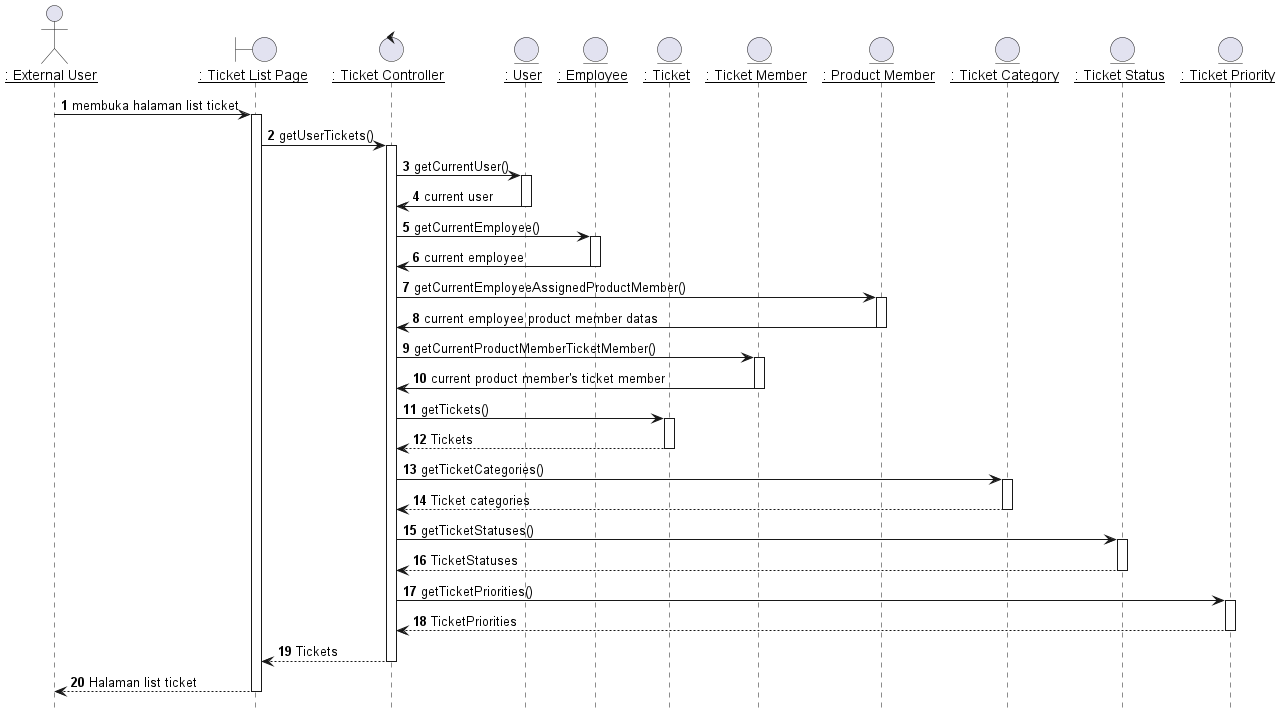
\includegraphics[width=\textwidth]{out/plantuml/sequence/ex/ex1/Melihat List Ticket.png}
                    \caption{Sequence Diagram Melihat List Ticket (External User)}
                    \label{fig:SQ-PIC-01}
                \end{sidewaysfigure}

                \begin{sidewaysfigure}
                    \centering 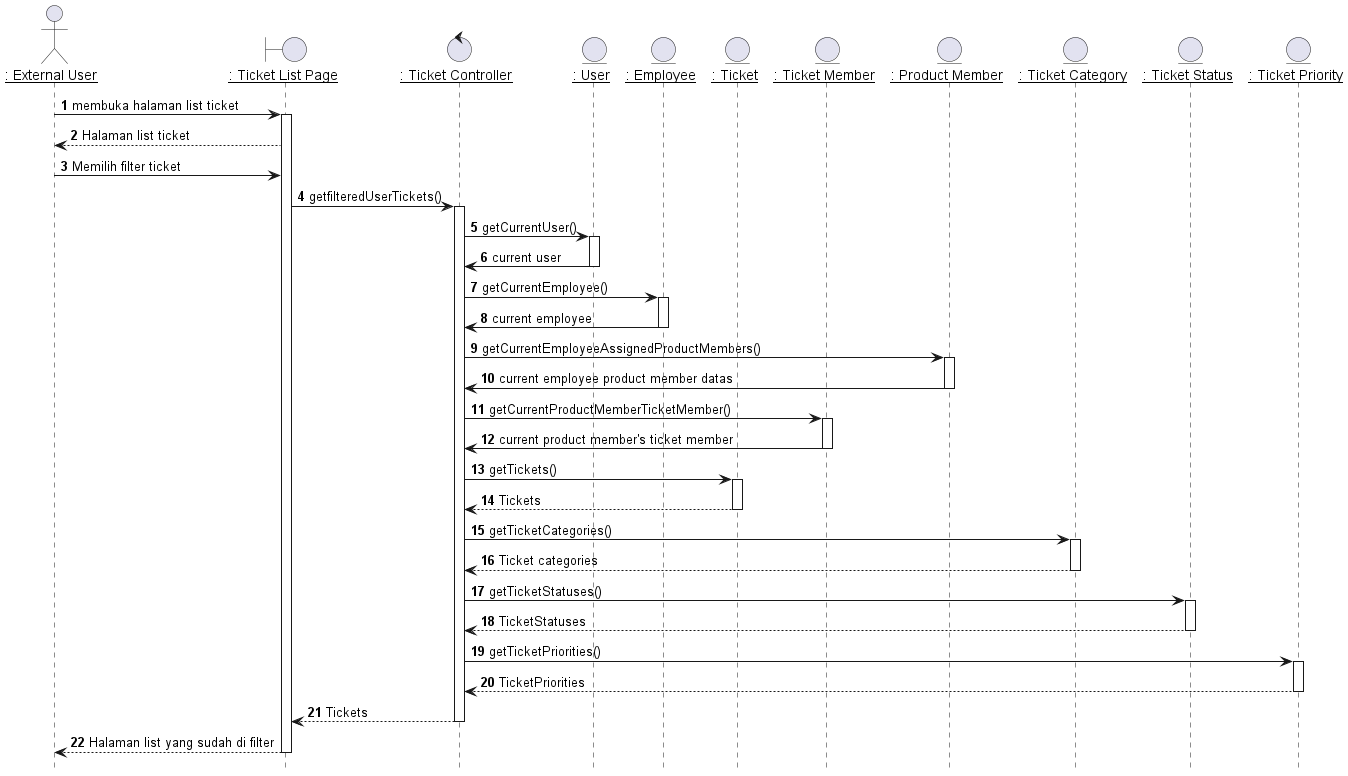
\includegraphics[width=\textwidth]{out/plantuml/sequence/ex/ex2/Memfilter List Ticket.png}
                    \caption{Sequence Diagram Memfilter List Ticket (External User)}
                    \label{fig:SQ-PIC-02}
                \end{sidewaysfigure}

                \begin{sidewaysfigure}
                    \centering 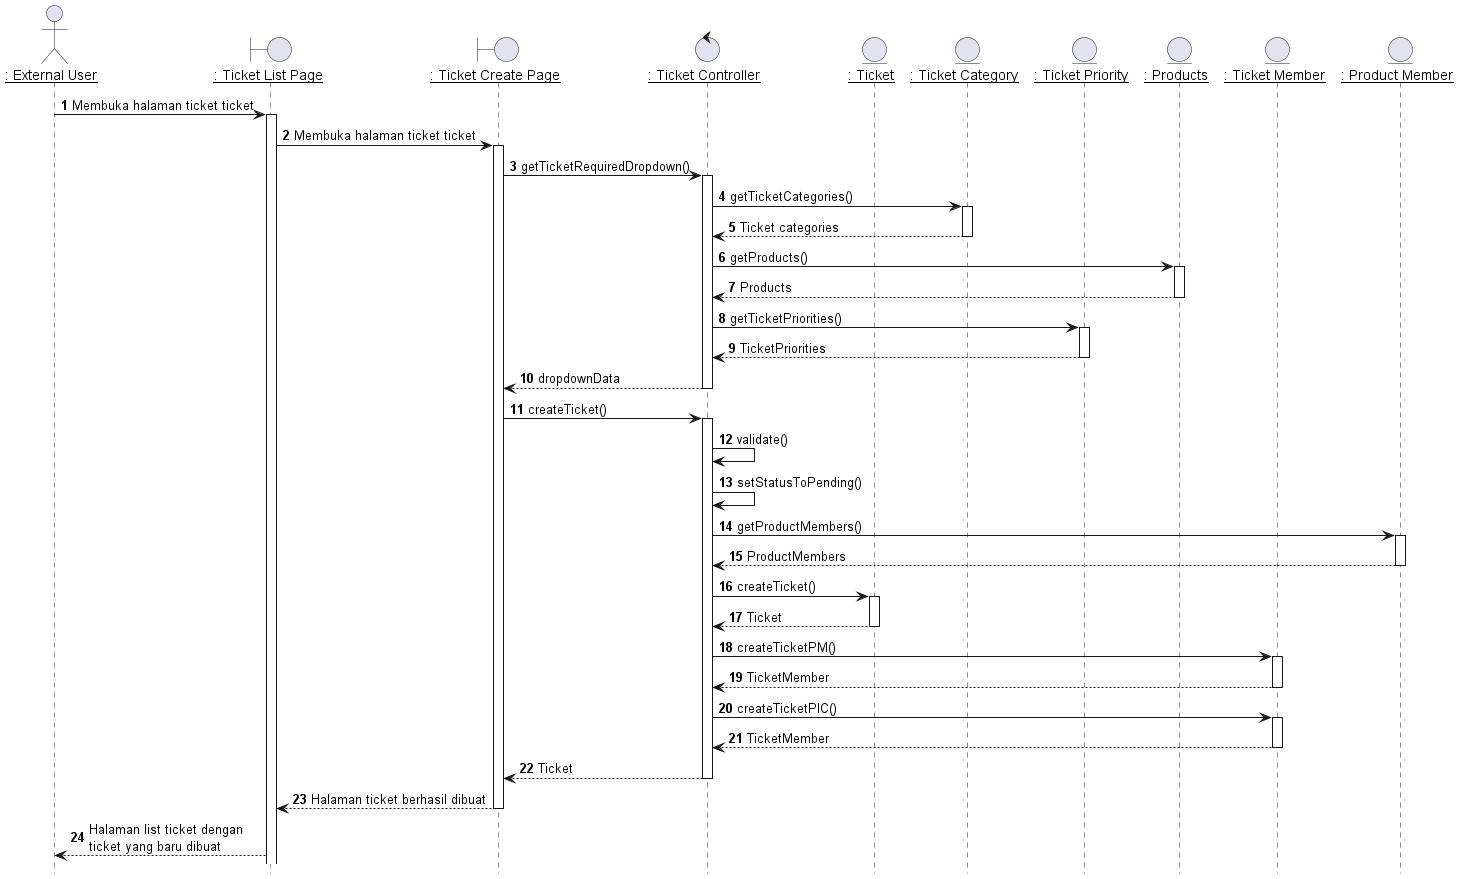
\includegraphics[width=\textwidth]{out/plantuml/sequence/ex/ex3/Membuat Ticket.png}
                    \caption{Sequence Diagram Membuat Ticket (External User)}
                    \label{fig:SQ-PIC-03}
                \end{sidewaysfigure}

                \begin{sidewaysfigure}
                    \centering 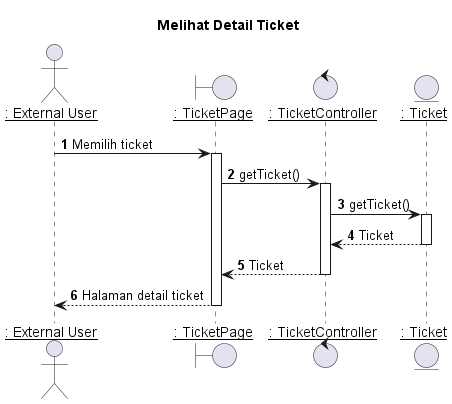
\includegraphics[width=\textwidth]{out/plantuml/sequence/ex/ex4/Melihat Detail Ticket.png}
                    \caption{Sequence Diagram Melihat Detail Ticket (External User)}
                    \label{fig:SQ-PIC-04}
                \end{sidewaysfigure}

                \begin{sidewaysfigure}
                    \centering 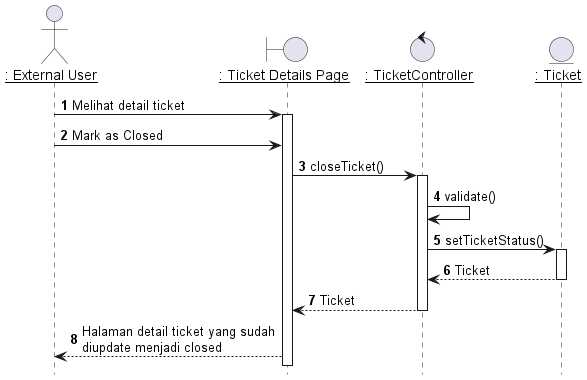
\includegraphics[width=\textwidth]{out/plantuml/sequence/ex/ex5/Menutup Ticket.png}
                    \caption{Sequence Diagram Menutup Ticket (External User)}
                    \label{fig:SQ-PIC-05}
                \end{sidewaysfigure}

                \begin{sidewaysfigure}
                    \centering 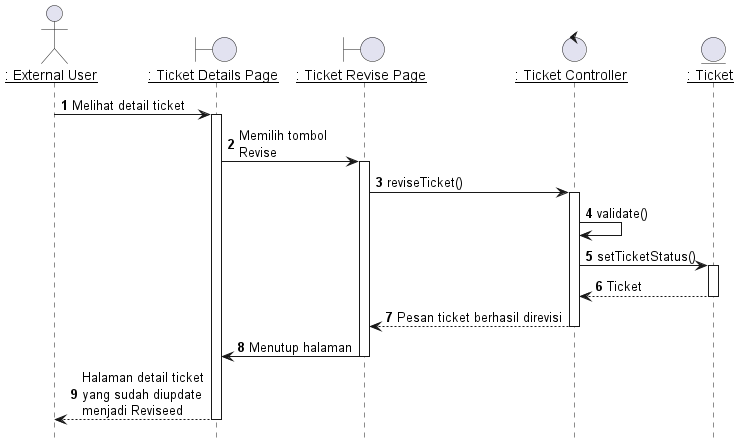
\includegraphics[width=\textwidth]{out/plantuml/sequence/ex/ex6/Merevisi Ticket.png}
                    \caption{Sequence Diagram Merevisi Ticket (External User)}
                    \label{fig:SQ-PIC-06}
                \end{sidewaysfigure}

                \begin{sidewaysfigure}
                    \centering 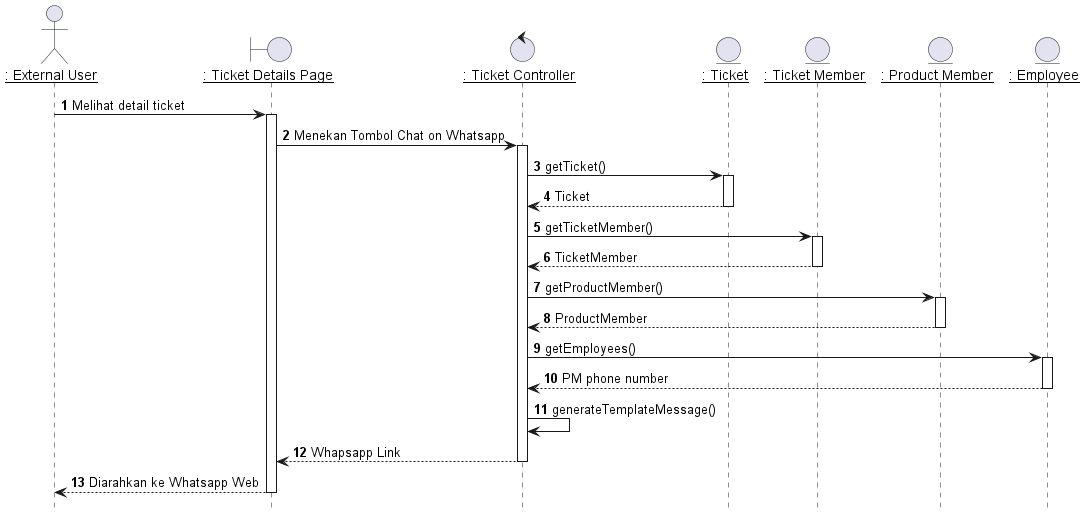
\includegraphics[width=\textwidth]{out/plantuml/sequence/ex/ex7/Berkomunikasi Dengan PM Melalui Whatsapp.png}
                    \caption{Sequence Diagram Berkomunikasi Dengan PM Melalui Whatsapp (External User)}
                    \label{fig:SQ-PIC-07}
                \end{sidewaysfigure}
            \end{enumerate}
        \end{enumerate}

        \newpage

        \listsection{Class Diagram}

            Class diagram merupakan diagram yang menggambarkan kelas-kelas yang akan digunakan dalam perangkat lunak beserta hubungan antar kelas. Setiap kelas memiliki nama kelas, atribut, dan metode dari kelas yang dibuat. Bagian ini akan membahas class diagram dari aplikasi Sistem Informasi Manajemen Produk dan Ticketing bagian modul ticketing yang telah dianalisa di bagian sequence diagram.

            \begin{enumerate}[label=\textbf{4.3.\arabic*.}]
                \listsection{Identifikasi Class}

                Identifikasi class class yang ada pada Sistem Informasi Manajemen Produk dan Ticketing bagian modul ticketing dapat dilihat pada tabel \ref{table:identifikasi-class}

                \begin{longtable}{ |l|l|l|p{0.6\textwidth}| }
                    \caption{Identifikasi Class} \label{table:identifikasi-class} \\
                    \hline
                    \textbf{No.} & \textbf{Stereotype} & \textbf{Nama Class} & \textbf{Deskripsi}\\
                    \hline
                    \endfirsthead
                  
                    \hline
                    \textbf{No.} & \textbf{Stereotype} & \textbf{Nama Class} & \textbf{Deskripsi}\\
                    \hline
                    \endhead
                  
                    1 & Entity & User & Entitas yang menyimpan informasi pengguna login. Seorang user menyimpan informasi login dan memiliki relasi ke employee yang dimiliki user ini.\\
                    \hline
                    2 & Entity & Employee & Entitas yang menyimpan informasi karyawan. Entitas ini berelasi 1:m dengan Product sebagai product manager dan berelasi 1:m dengan ProductMember sebagai member dari sebuah Product \\
                    \hline
                    3 & Entity & Product & Entitas yang menyimpan informasi suatu produk. Entitas ini berelasi 1:m dengan ticket untuk aggregasi ticket pada product serta berelasi 1:m dengan ProductMember untuk aggregasi employee yang bekerja pada product ini \\
                    \hline
                    4 & Entity & Ticket & Entitas yang menyimpan informasi ticket, berelasi m:n dengan ProductMember karena tiap product member bisa saja mengerjakan banyak ticket dan tiap ticket bisa saja dikerjakan banyak product member. \\
                    \hline
                    5 & Entity & TicketMember & Entitas yang menyimpan informasi mengenai ProductMember yang mengerjakan suatu ticket. Class ini juga menyimpan status pengerjaan dari Employee yang mengerjakan ticket tersebut \\
                    \hline
                    6 & Entity & TicketCategory & Entitas yang menyimpan informasi mengenai kategori dari suatu ticket. \\
                    \hline
                    7 & Entity & TicketStatus & Entitas yang menyimpan informasi mengenai status dari suatu ticket. \\
                    \hline
                    8 & Entity & TicketPriority & Entitas yang menyimpan informasi mengenai prioritas dari suatu ticket. \\
                    \hline
                    9 & Entity & ProductMember & Entitas yang memberikan role dari employee yang bekerja di suatu product \\
                    \hline
                    10 & Control & TicketController & Class control yang menyediakan manipulasi data dan perantara antara entity dan boundary ticketing \\
                    \hline
                    11 & Boundary & TicketCreatePage & Page yang menyediakan form pembuatan ticket \\
                    \hline
                    12 & Boundary & TicketDetailsPage & Page yang menampilkan detail ticket serta transaksi ticket berupa verify, reject, done, dan close juga menyediakan form assign developer. \\
                    \hline
                    13 & Boundary & TicketListPage & Page yang menampilkan list ticket yang berguna sebagai mulai alur transaksi ticketing. \\
                    \hline
        
                \end{longtable}

                \listsection{Class Diagram}

                Setelah mendefinisikan class yang terlibat pada identifikasi class, tahap selanjutnya adalah memodelkan class diagram berupa visualisasi yang terdiri atas entitas, method dan relasi antar class yang dapat dilihat pada gambar \ref{fig:class-diagram}.

                \begin{figure}[H]
                    \centering 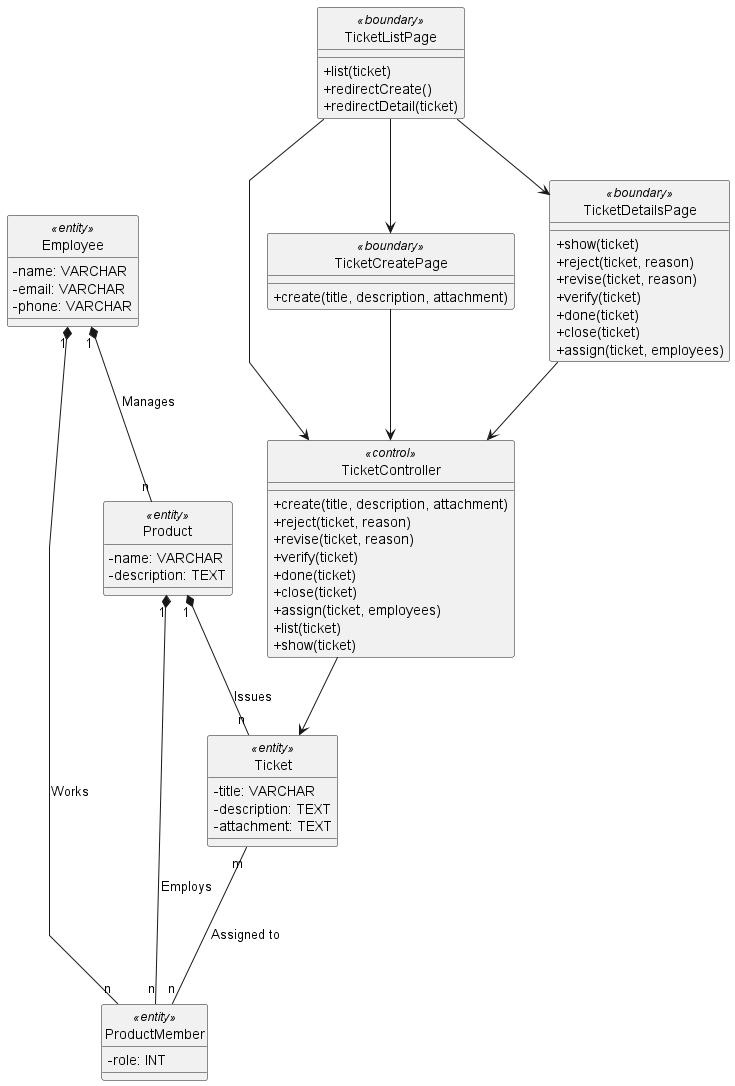
\includegraphics[width=0.9\textwidth]{out/plantuml/class_diagram/class diagram.png}
                    \caption{Class Diagram Modul Ticketing}
                    \label{fig:class-diagram}
                \end{figure}


            \end{enumerate}

  
          
    \end{enumerate}

    \listsection{Design}

    Eksplorasi mendalam mengenai desain arsitektural dari sistem yang sedang dikembangkan akan dilakukan. Untuk memastikan pemahaman yang komprehensif mengenai integrasi dan interaksi antar-komponen dalam aplikasi, dua bentuk diagram utama akan diperkenalkan: Package Diagram dan Deployment Diagram. Package Diagram akan menguraikan struktur organisasi dan modularisasi dari komponen-komponen sistem, menunjukkan pemecahan dan pengelompokan fungsi-fungsi sistem. Deployment Diagram akan menyediakan perspektif terkait dengan distribusi fisik sumber daya komputasi yang digunakan oleh aplikasi serta cara berkomunikasi antar-komponen di lingkungan produksi. Pemaparan ini bertujuan untuk mendukung analisis terhadap aspek skalabilitas, performa, dan keamanan sistem, sehingga memberikan gambaran yang lebih jelas dan menyeluruh tentang kerangka kerja arsitektural yang dipilih.
    
    \begin{enumerate} [label=\textbf{4.3.\arabic*.}, wide, labelwidth=!, labelindent=0pt]
        \listsection{Package Diagram}

        Package Diagram digunakan untuk mengilustrasikan organisasi struktural serta hubungan antar komponen yang ada dalam Sistem IT Service Desk di PT Teknologi Aplikasi Sejahtera.  

        \listsection{Deployment Diagram}

        Deployment diagram ini memberikan visualisasi tentang bagaimana aplikasi di-deploy dalam lingkungan produksi, termasuk perangkat keras dan perangkat lunak yang digunakan dalam mendistribusikan dan menjalankan komponen aplikasi. Deployment diagram Sistem Informasi Manajemen Produk dan Ticketing dapat dilihat pada gambar \ref{fig:deployement-diagram}.
        
        \begin{figure}[H]
            \centering 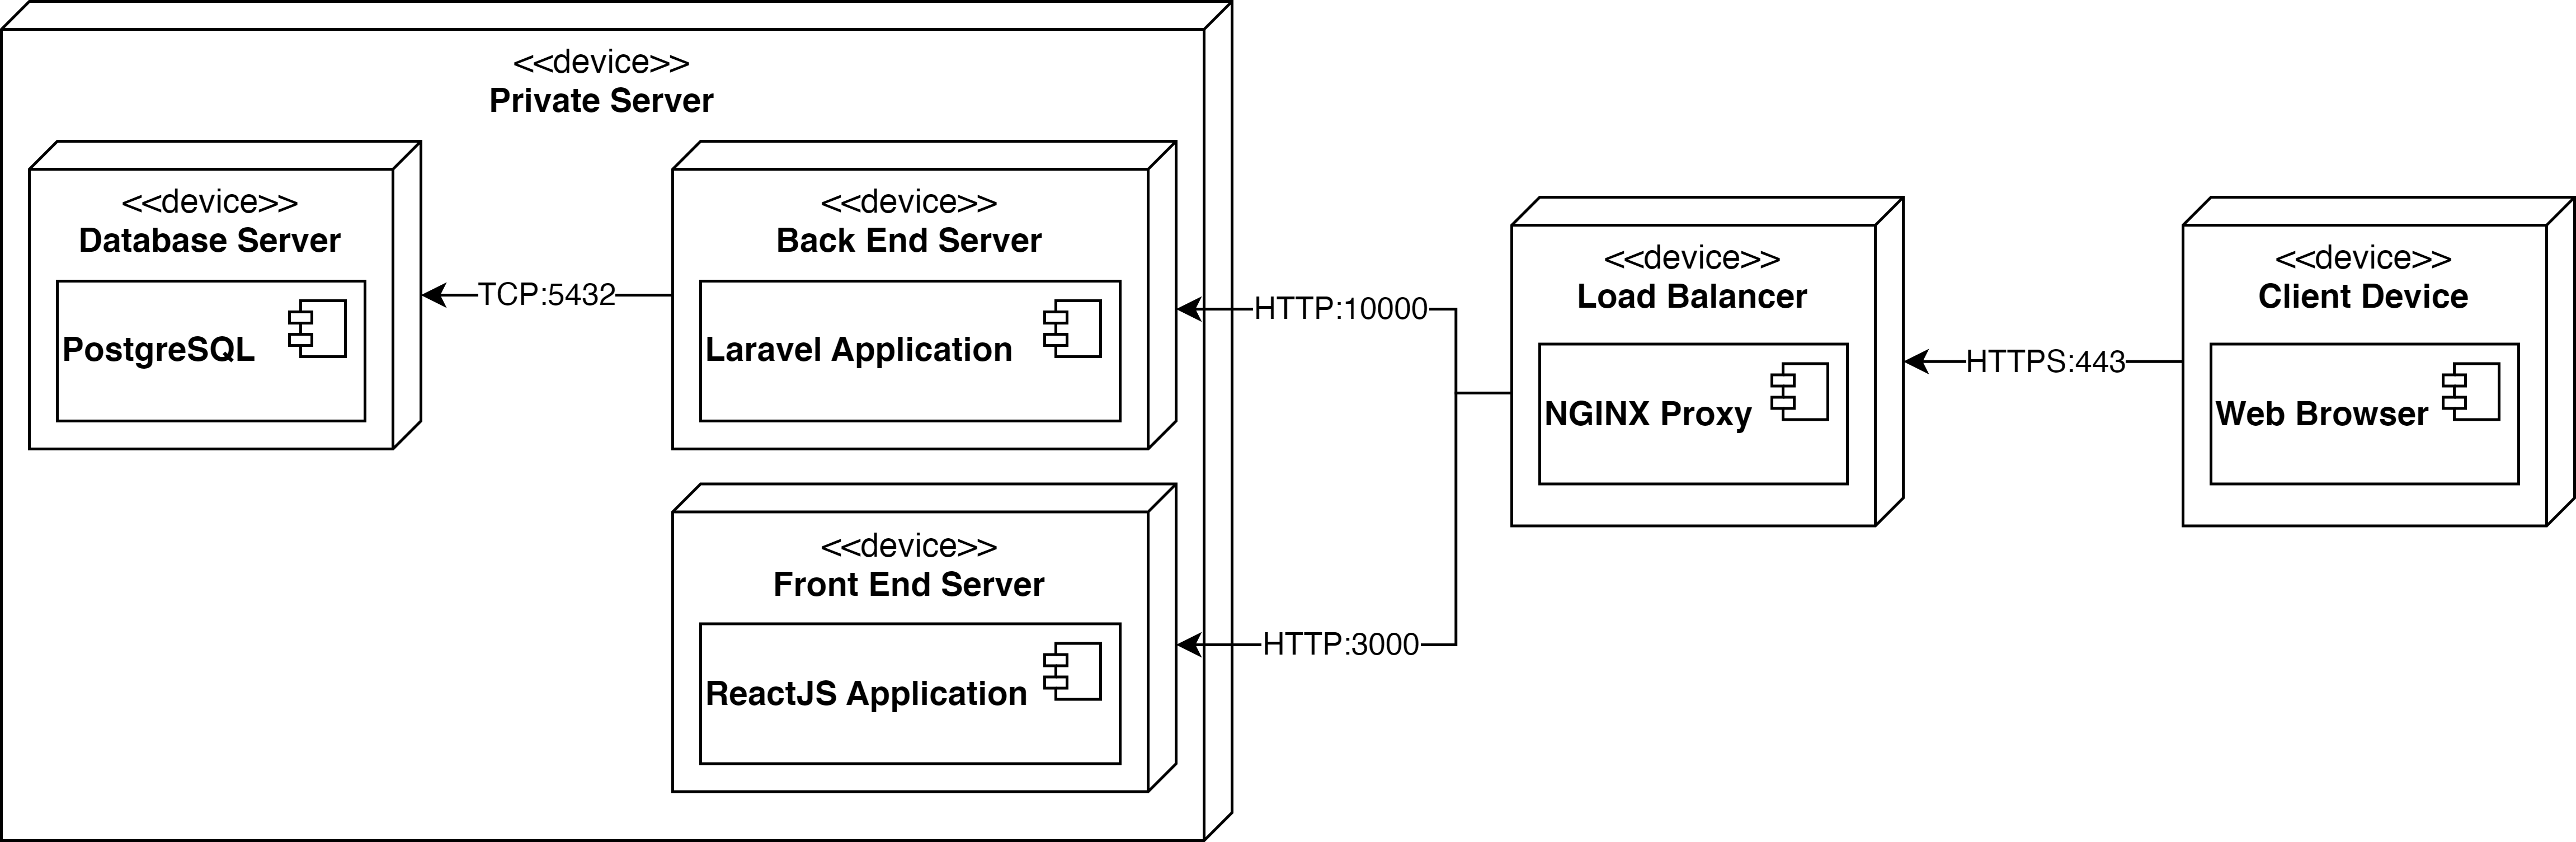
\includegraphics[width=0.9\textwidth]{images/deployment.png}
            \caption{Deployment Diagram}
            \label{fig:deployement-diagram}
        \end{figure}

        Diagram diatas menunjukkan bagian bagian utama deployment Sistem Informasi Manajemen Produk dan Ticketing. Penjelasan untuk masing masing komponen akan dijelaskan sebagai berikut:

        \begin{enumerate}[label=\arabic*.]
            \item Private Server
            
            Private server merupakan device utama yang digunakan sebagai host dari backend server, frontend server, dan database server. Mesin ini memiliki kemampuan komputasi yang tinggi dengan ram yang cukup besar. Alasan private server melakukan virtualisasi ini adalah untuk memungkinkan isolasi antar service dan dapat mengalokasikan sumber daya dengan efisien, sehingga setiap service yang dibuat server dapat dikelola secara independen dan fleksibel. Penggunaan satu mesin seperti ini dapat memudahkan untuk memanage service yang ada pada satu device. Namun, dengan hanya ada satu mesin saja skalabilitas aplikasi menjadi terbatas.


            \item Database Server dan PostgreSQL
            
            Database server perangkat yang dirancang khusus untuk menyediakan layanan database kepada backend server. Database server dipisah dengan backend dengan tujuan tim pengembang dapat menggunakan database bersama tanpa menghiraukan masa pemeliharaan server backend. Database server beroperasi sebagai virtual machine di bawah private server.
            
            Database server memiliki satu layanan yakni PostgreSQL. PostgreSQL akan digunakan sebagai sumber penyimpanan persistent backend server.

            \item Backend Server dan Laravel Application
            
            Backend server merupakan perangkat yang akan digunakan sebagai penyedia layanan backend dari Sistem Informasi Manajemen Produk dan Ticketing. Backend server akan lebih berfokus pada manipulasi data yang persisten serta mengatur logika bisnis. Untuk implementasinya, tim pengembang memilih menggunakan PHP dengan framework Laravel sebagai backend.
            
            \item Frontend Server dan React.JS Application
            
            Frontend server merupakan perangkat yang akan digunakan sebagai penyedia layanan frontend dari Sistem Informasi Manajemen Produk dan Ticketing. Berbeda dari backend, frontend lebih berfokus kepada bagaimana data disajikan dan ditampilkan. Untuk implementasinya, tim pengembang memilih menggunakan React.JS sebagai framework frontend.
            
            \item Load Balancer dengan NGINX Proxy
            
            Load balancer digunakan sebagai penyeimbang beban requests yang masuk. Load balancer akan di-host di layanan cloud yang memiliki IP publik. Selain sebagai penyeimbang beban, mesin ini juga akan digunakan sebagai gateway akses ke bagian private server karena private server tidak memiliki IP publik yang statis. Dengan menggunakan NGINX proxy, mesin dapat meneruskan request sesuai service yang dituju meskipun berada di IP yang sama namun dengan domain yang berbeda.

            \item PC Client dan Web Browser
            
            PC client merupakan device yang digunakan pengguna untuk mengakses Sistem Informasi Manajemen Produk dan Ticketing. Pengguna akan memasukkan url ke dalam navigasi web browser yang akan melakukan request ke frontend server dan backend server melalu load balancer.
            

        \end{enumerate}


        \listsection{Desain Antarmuka Aplikasi}

        Berikut merupakan penjelasan rancangan desain antarmuka Sistem Informasi Manajemen Produk dan Ticketing bagian ticketing di PT. Teknologi Aplikasi Sejahtera:

        \begin{enumerate}[label=\arabic*.]
            \item Halaman List Ticket
            
            Pada halaman list ticket akan ditampilkan list ticket yang user sedang login memiliki tanggung jawab. Semisal sebagai PM maka seluruh tiket product yang di assign akan muncul dan jika sebagai external user maka semua ticket yang ia buat akan muncul di sini. Sebagai tambahan user dapat melakukan searching menggunakan kolom search. User juga bisa melakukan filter berdasarkan statusnya. User juga bisa melakukan sorting berdasarkan seberapa baru ticket itu dibuat. Jika user merasa tampilan dalam satu halaman terlalu sedikit atau terlalu banyak, user juga bisa mengatur banyaknya ticket yang ditampilkan dalam satu halaman. Khusus untuk external user, akan muncul tombol new ticket untuk membuat ticket baru. Tampilan mockup ui halaman list ticket dapat dilihat pada gambar \ref{fig:figma-list}.
        
            \begin{figure}[H]
                \centering 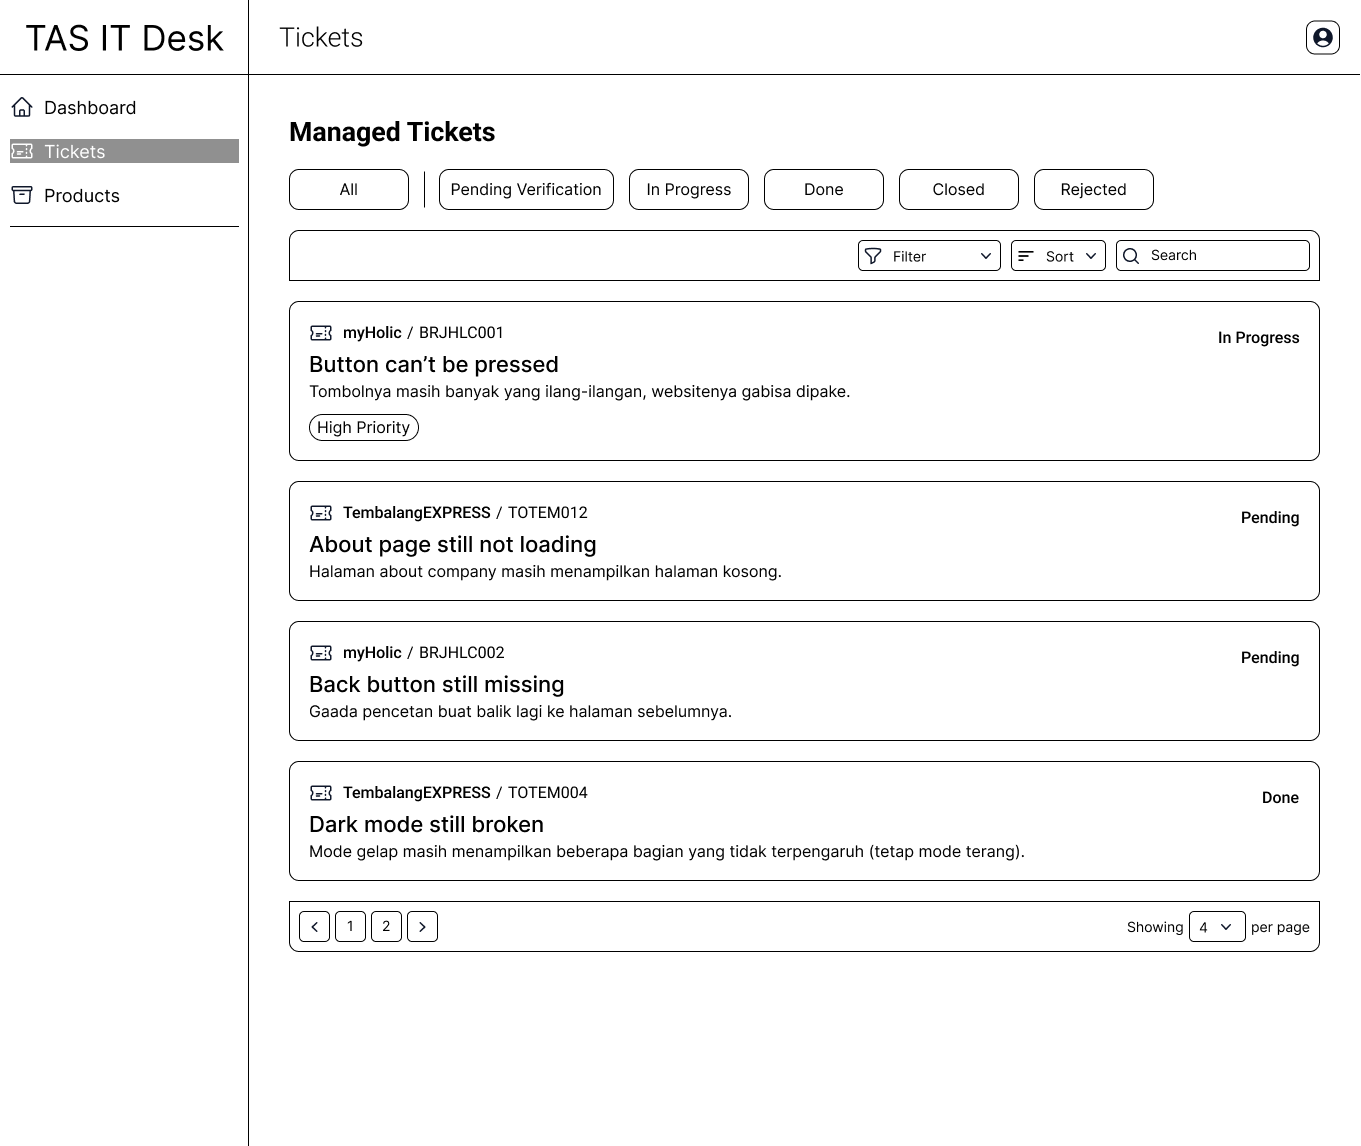
\includegraphics[width=0.9\textwidth]{images/figma/[Project Manager] Tickets.png}
                \caption{Prototype List Ticket}
                \label{fig:figma-list}
            \end{figure}

            \item Halaman Membuat Ticket
        
            Untuk external user yang ingin membuat ticket, akan diteruskan ke halaman ini, user akan mengisi informasi yang diperlukan untuk membuat ticket dengan field yang wajib adalah project, tingkat prioritas, judul atau nama ticket, serta deskripsi permasalahan. User dapat menambahkan attachment untuk memberikan tambahan informasi jika tidak dapat dijelaskan menggunakan kata kata. Tampilan mockup ui halaman pembuatan ticket dapat dilihat pada gambar \ref{fig:figma-create}.

            \begin{figure}[H]
                \centering 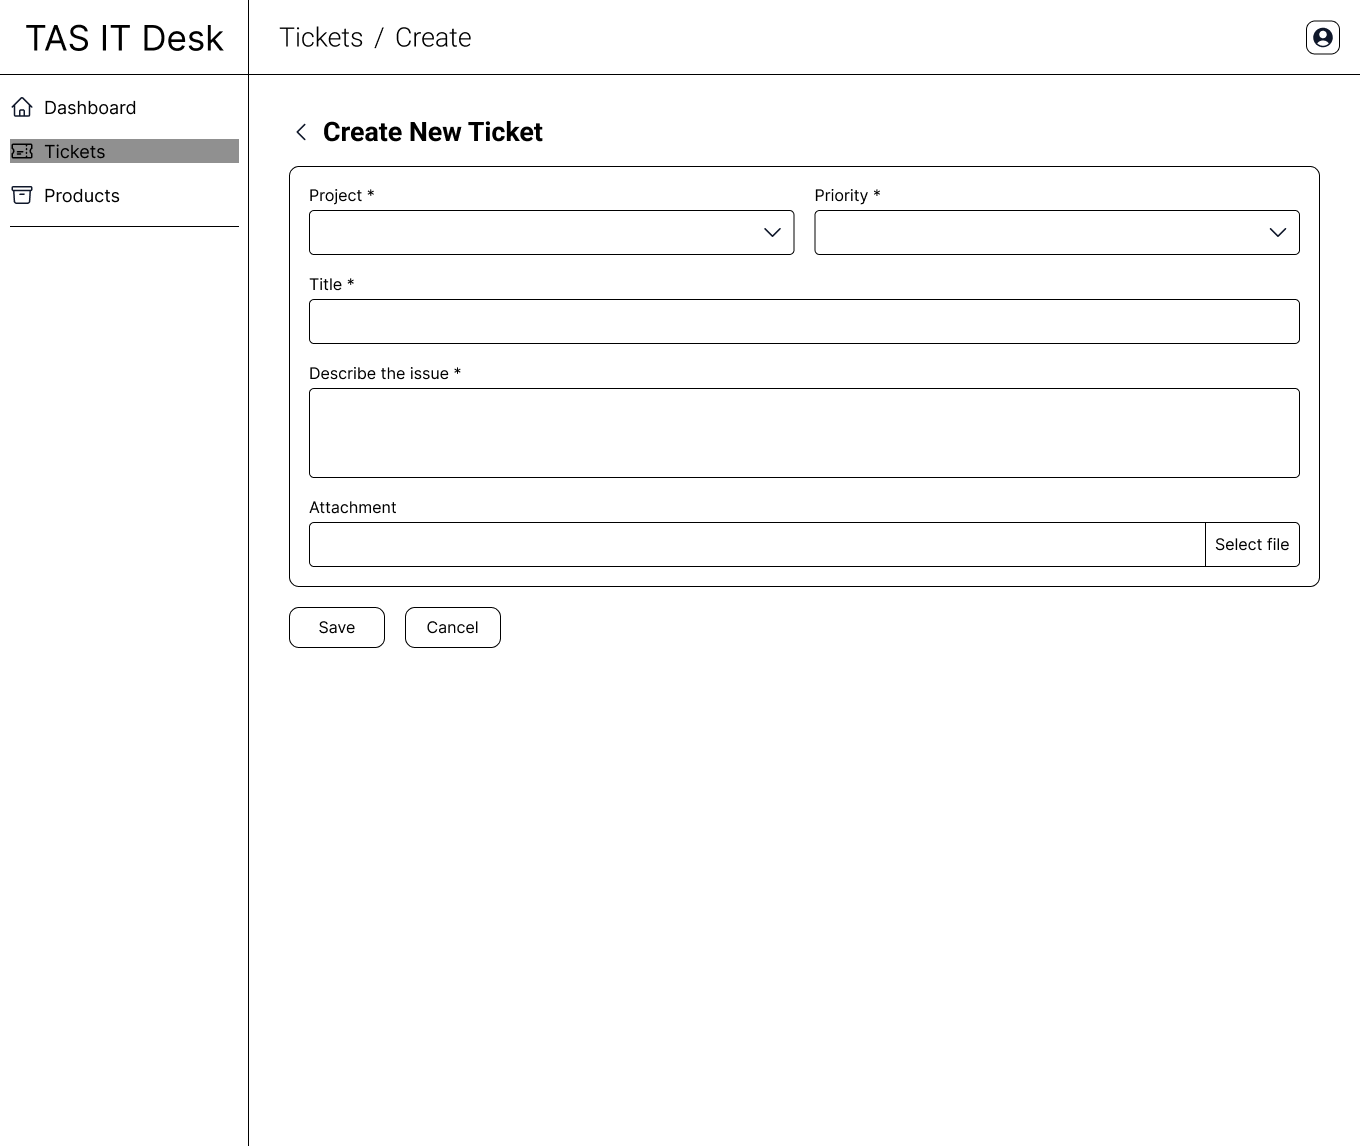
\includegraphics[width=0.9\textwidth]{images/figma/[Client] Ticket Create.png}
                \caption{Prototype Create Ticket}
                \label{fig:figma-create}
            \end{figure}
        

            \item Halaman Detail Ticket

            Halaman ini adalah halaman di mana transaksi ticket berlangsung. Fungsionalitas halaman ini akan berubah tergantung role user dan kondisi ticket. Ketika ticket menunggu verifikasi, hanya product manager yang dapat memverifikasi ticket tersebut atau menolak ticket tersebut. Jika product manager memilih untuk memverifikasi ticket tersebut, akan muncul popup untuk memilih developer mana yang akan mengerjakan ticket tersebut. Developer yang mengerjakan ticket tersebut dapat melaporkan pekerjaannya dengan menekan tombol done. Setelah semua developer sudah OK, product manager dapat melakukan pengecekan apakah pekerjaan sudah selesai dan benar. Jika belum progress pekerjaan developer akan direset ulang. Jika sudah, ticket akan ke tahap selanjutnya untuk divalidasi dari sisi client atau pembuat ticket. Jika tidak sesuai maka akan dikembalikan ke fase pengerjaan, jika sesuai ticket akan menjadi closed. Tampilan mockup ui halaman detail ticket dapat dilihat pada gambar \ref{fig:figma-details}.

            \begin{figure}[H]
                \centering 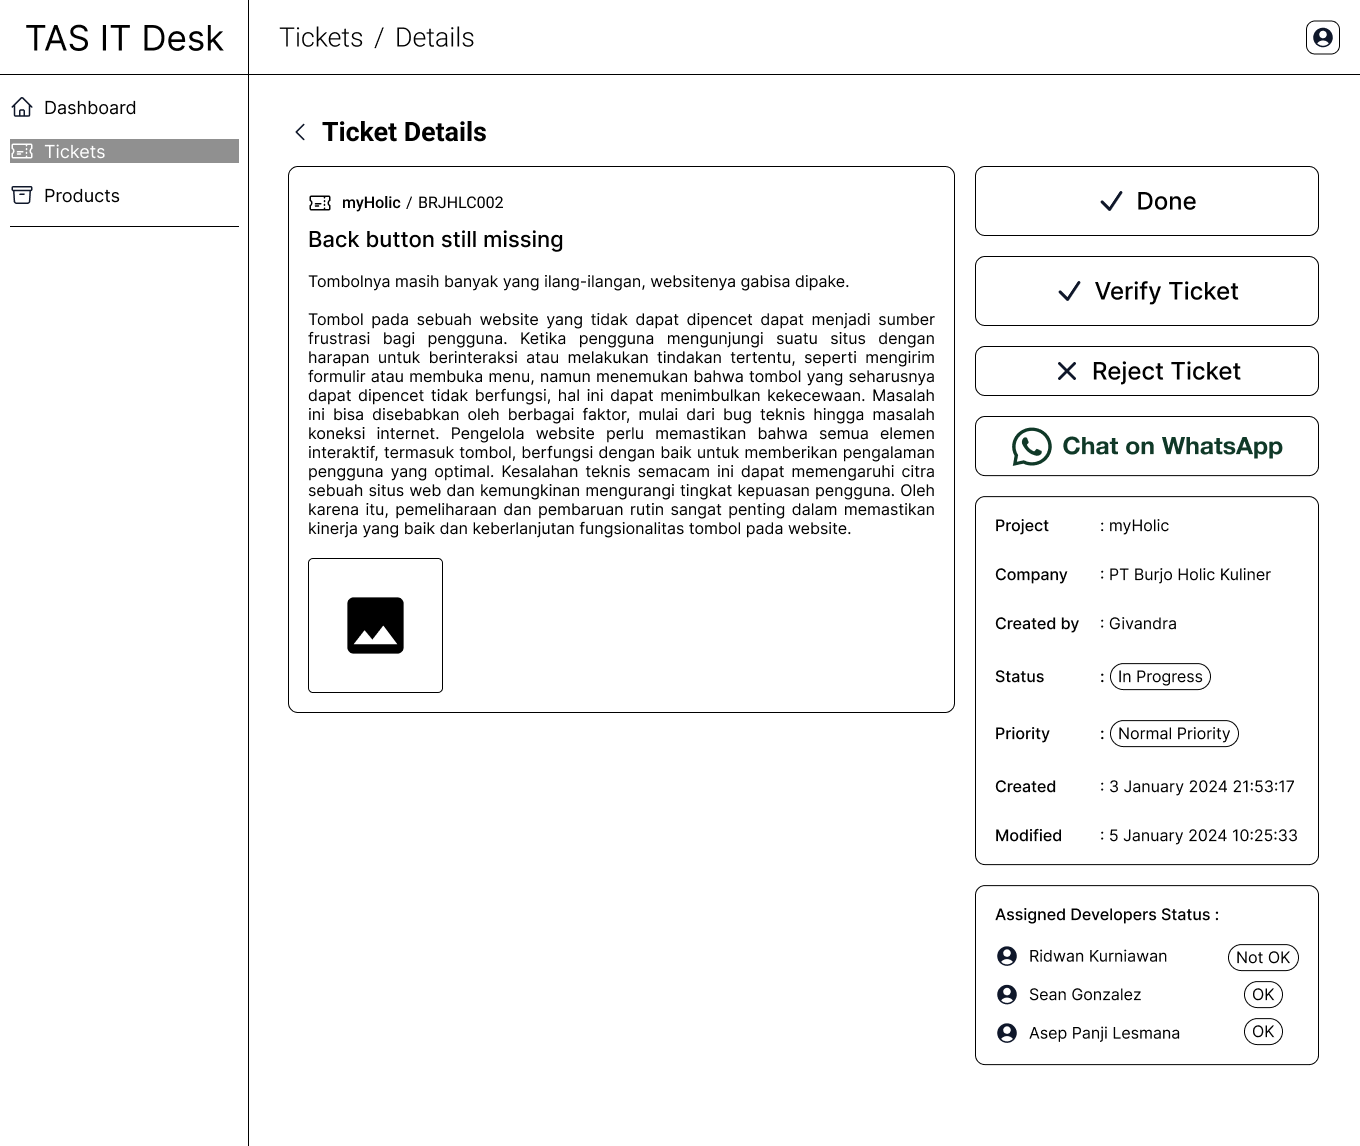
\includegraphics[width=0.9\textwidth]{images/figma/[Project Manager] Tickets Details.png}
                \caption{Prototype Ticket Details}
                \label{fig:figma-details}
            \end{figure}

            \item Popup Verify Ticket
            

            \begin{figure}[H]
                \centering 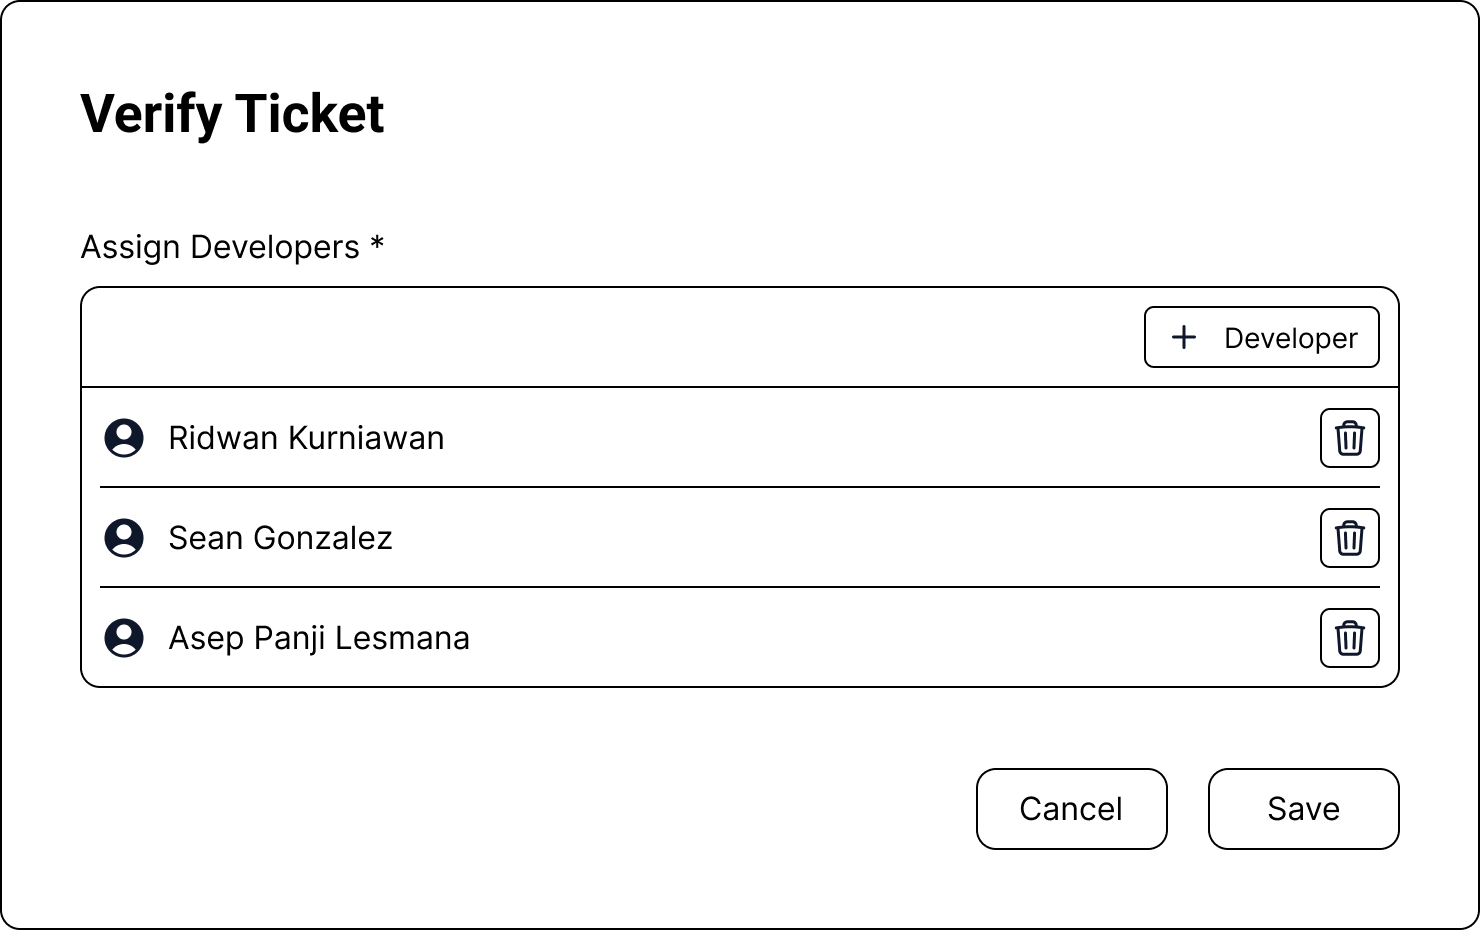
\includegraphics[width=0.9\textwidth]{images/figma/Verify Ticket.png}
                \caption{Prototype Popup Verify Ticket}
                \label{fig:figma-verify}
            \end{figure}
            
            \item Popup Reject Ticket
            
            \begin{figure}[H]
                \centering 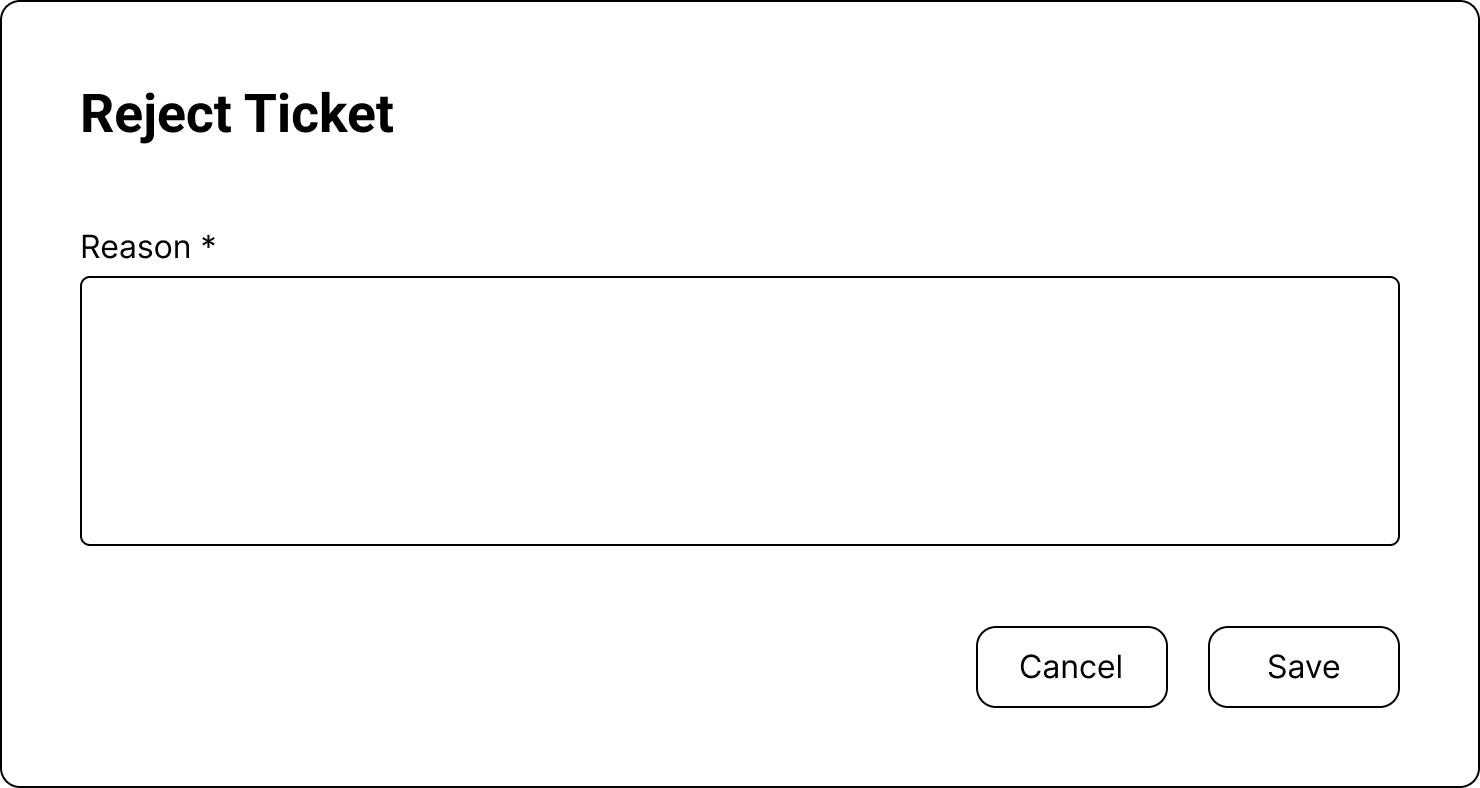
\includegraphics[width=0.9\textwidth]{images/figma/Reject Ticket.png}
                \caption{Prototype Popup Reject Ticket}
                \label{fig:figma-reject}
            \end{figure}
            
            \item Popup Revise Ticket
            
            \begin{figure}[H]
                \centering 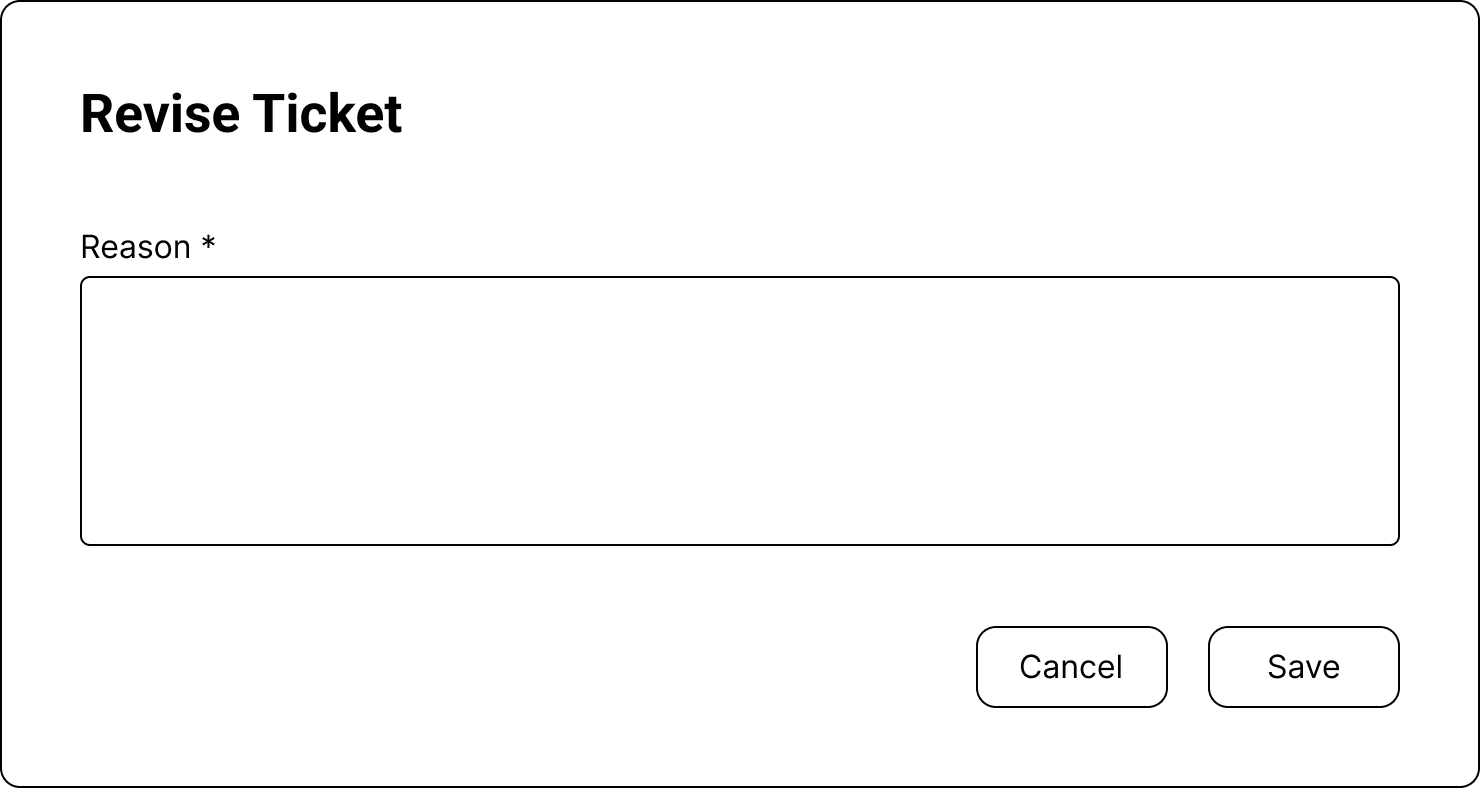
\includegraphics[width=0.9\textwidth]{images/figma/Revise Ticket.png}
                \caption{Prototype Popup Revise Ticket}
                \label{fig:figma-revise}
            \end{figure}


        \end{enumerate}
    \end{enumerate}

    asd \citep{doe2021} dan  \citep{smith2020}

    
    \newpage

\end{enumerate}


\newpage

%  ██      ██     ██      ████████ ██ ██
% ░██     ░██    ████    ██░░░░░░ ░██░██
% ░██     ░██   ██░░██  ░██       ░██░██
% ░██████████  ██  ░░██ ░█████████░██░██
% ░██░░░░░░██ ██████████░░░░░░░░██░██░██
% ░██     ░██░██░░░░░░██       ░██░██░██
% ░██     ░██░██     ░██ ████████ ░██░████████
% ░░      ░░ ░░      ░░ ░░░░░░░░  ░░ ░░░░░░░░

%  ███████       ██     ████     ██
% ░██░░░░██     ████   ░██░██   ░██
% ░██    ░██   ██░░██  ░██░░██  ░██
% ░██    ░██  ██  ░░██ ░██ ░░██ ░██
% ░██    ░██ ██████████░██  ░░██░██
% ░██    ██ ░██░░░░░░██░██   ░░████
% ░███████  ░██     ░██░██    ░░███
% ░░░░░░░   ░░      ░░ ░░      ░░░

%  ███████  ████████ ████     ████ ██████       ██     ██      ██     ██
% ░██░░░░██░██░░░░░ ░██░██   ██░██░█░░░░██     ████   ░██     ░██    ████
% ░██   ░██░██      ░██░░██ ██ ░██░█   ░██    ██░░██  ░██     ░██   ██░░██
% ░███████ ░███████ ░██ ░░███  ░██░██████    ██  ░░██ ░██████████  ██  ░░██
% ░██░░░░  ░██░░░░  ░██  ░░█   ░██░█░░░░ ██ ██████████░██░░░░░░██ ██████████
% ░██      ░██      ░██   ░    ░██░█    ░██░██░░░░░░██░██     ░██░██░░░░░░██
% ░██      ░████████░██        ░██░███████ ░██     ░██░██     ░██░██     ░██
% ░░       ░░░░░░░░ ░░         ░░ ░░░░░░░  ░░      ░░ ░░      ░░ ░░      ░░
%   ████████     ██     ████     ██
%  ██░░░░░░     ████   ░██░██   ░██
% ░██          ██░░██  ░██░░██  ░██
% ░█████████  ██  ░░██ ░██ ░░██ ░██
% ░░░░░░░░██ ██████████░██  ░░██░██
%        ░██░██░░░░░░██░██   ░░████
%  ████████ ░██     ░██░██    ░░███
% ░░░░░░░░  ░░      ░░ ░░      ░░░

\section[BAB V HASIL DAN PEMBAHASAN]{BAB V\\HASIL DAN PEMBAHASAN}

\setcounter{table}{0}
\setcounter{figure}{0}

\begin{enumerate}[label=\textbf{5.\arabic*.}]
    \listsection{Implementasi Sistem}

        
    Spesifikasi perangkat keras dan lunak yang digunakan dalam mengembangkan Sistem Informasi Manajemen Produk dan Ticketing bagian ticketing di PT. Teknologi Aplikasi Sejahtera.

    \begin{table}[h!]
        \caption{Informasi Hardware pengembangan}
        \centering
        \begin{tabularx}{\linewidth}{ |l|X| }
            \hline
            CPU                        & Intel(R) Core(TM) i7-9750H CPU @ 2.60GHz \\ %\addlinespace
            \hline
            Sistem Operasi             & Microsoft Windows 10 Home Single Language build 19045 \\ %\addlinespace
            \hline
            Bahasa pemograman          & PHP dan Javascript \\ %\addlinespace
            \hline
            Framework frontend         & React.js\\ %\addlinespace
            \hline
            Framework backend          & Laravel \\ %\addlinespace
            \hline
            Database Management System & PostgreSQL \\ %\addlinespace
            \hline
            IDE                        & Visual Studio Code \\ %\addlinespace
            \hline
            Web browser                & Google Chrome \\ %\addlinespace
            \hline
        \end{tabularx}
        \label{table:hardware-pengembangan}
    \end{table}

    \begin{enumerate}[label=\textbf{5.1.\arabic*.}]
        \listsection{Implementasi Antarmuka Ticketing}

        \begin{enumerate}[label=\textbf{5.1.1.\arabic*.}]
            \listsection{Antarmuka List Ticket}

            Halaman list ticket merupakan halaman utama dari modul ticketing di Sistem Informasi Manajemen Produk dan Ticketing. Pada halaman ini akan ditampilkan informasi mengenai ticket yang user tersebut memiliki tanggung jawab. Di halaman ini user dapat diberikan opsi untuk mencari dan memfilter kategori tiket yang ingin dicari. Sistem memberikan opsi untuk memfilter berdasarkan kategori dan status. User juga dapat mengurutkan berdasarkan kronologi pembuatan dan modifikasi. Pada halaman ini jika user merupakan seorang external user, sistem akan menampilkan tombol untuk membuat ticket baru yang akan diarahkan ke halaman membuat ticket. Desain antarmuka list ticket dapat dilihat pada gambar \ref{fig:antarmuka-list}.

            \begin{figure}[H]
                \centering 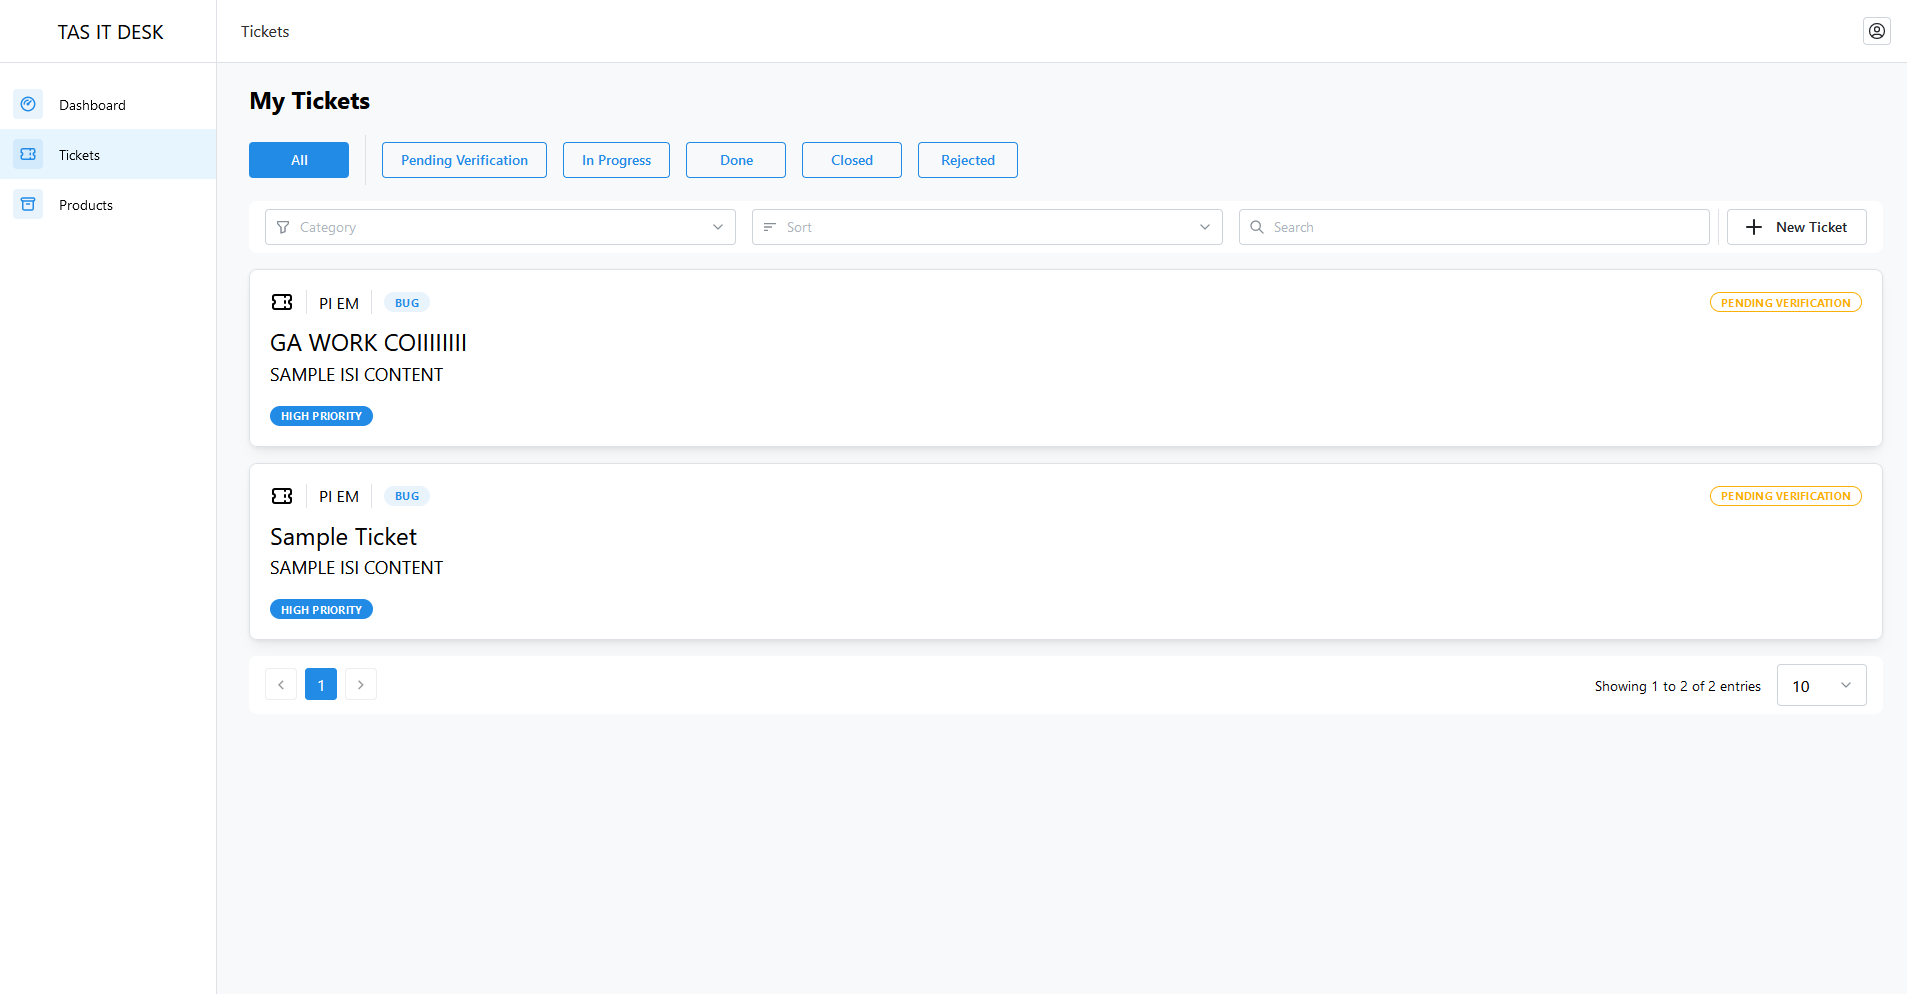
\includegraphics[width=\textwidth]{images/antarmuka/list.png}
                \caption{Antarmuka List Ticket}
                \label{fig:antarmuka-list}
            \end{figure}

            \listsection{Antarmuka Membuat Ticket}
            
            Halaman pembuatan ticket merupakan halaman yang berasal dari halaman list ticket. Halaman ini hanya dapat diakses oleh seorang external user. Pada halaman ini user akan diberikan form untuk mengisikan informasi yang diperlukan untuk membuat ticket seperti product apa, prioritas dari ticket tersebut, kategori ticket, judul dari ticket, serta deskripsi kenapa ticket tersebut perlu dibuat.

            \begin{figure}[H]
                \centering 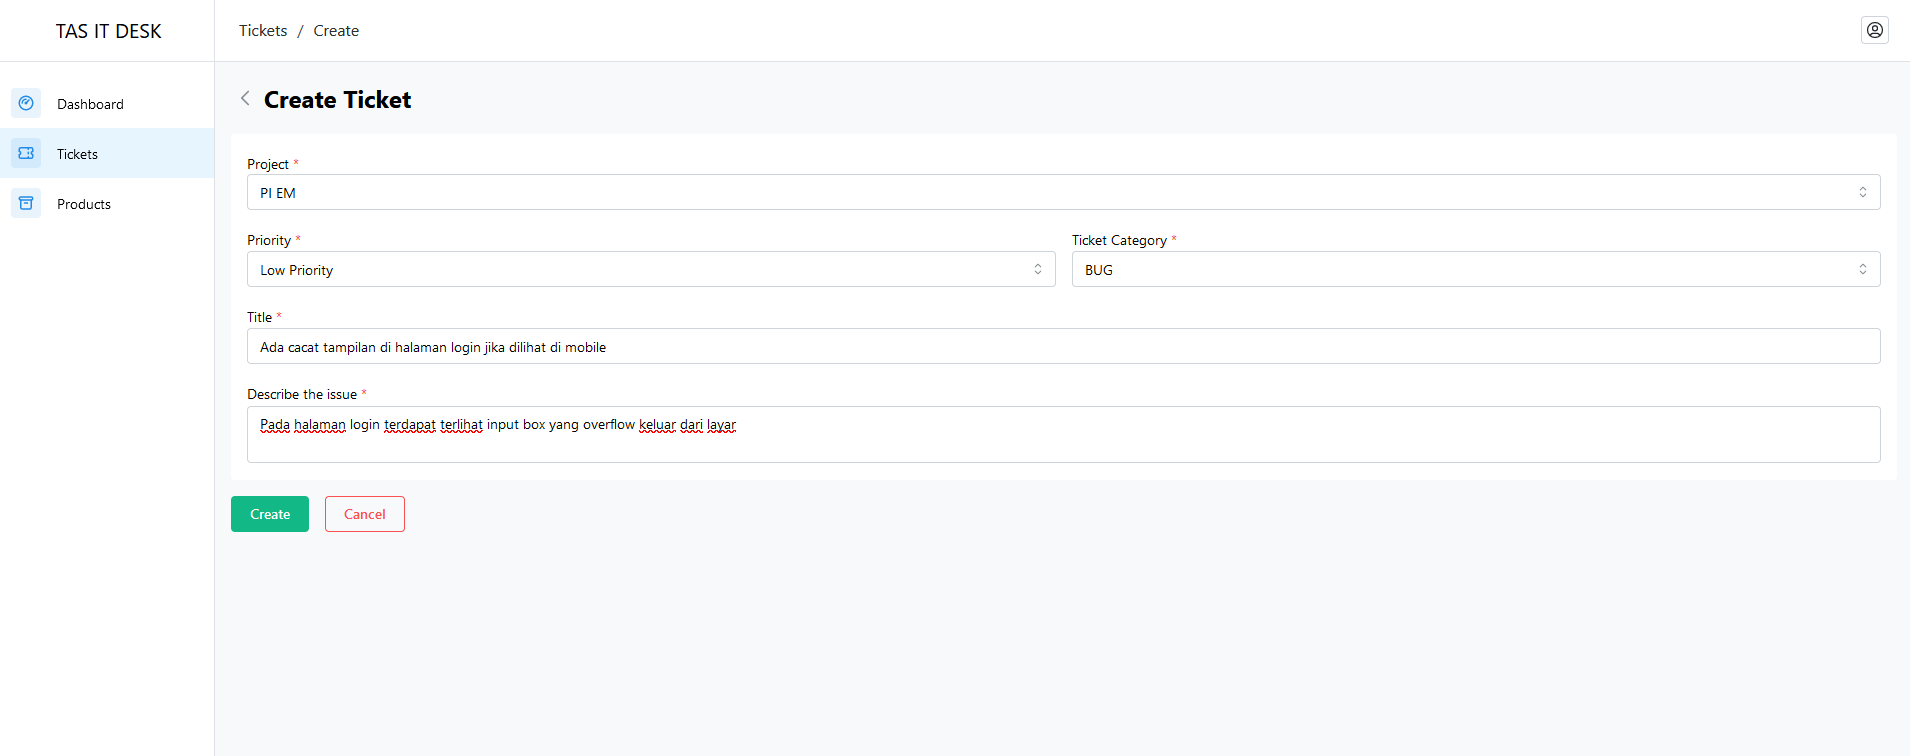
\includegraphics[width=\textwidth]{images/antarmuka/create.png}
                \caption{Antarmuka Membuat Ticket}
                \label{fig:antarmuka-create}
            \end{figure}

            \listsection{Antarmuka Detail Ticket}

            Halaman detail ticket memberikan informasi keseluruhan ticket tersebut. Informasi yang disampaikan berupa deskripsi ticket, judul ticket, status ticket, prioritas ticket, kategori ticket, dari product apa, dari company apa, siapa yang membuat, kapan di buat, kapan ada aktivitas terbaru di ticket tersebut, siapa yang mengerjakan, serta status pengerjaannya. User dengan role external user dapat merevisi dan menutup ticket yang ia buat. User dengan role product manager dapat memverifikasi atau mereject ticket yang baru dibuat, setelah dikerjakan product manager juga dapat memvalidasi pekerjaan developer dengan mengubah status menjadi done atau merevisi ulang. User dengan role developer hanya dapat mengubah status pengerjaan menjadi done untuk tugasnya. 

            \begin{figure}[H]
                \centering \includegraphics[width=\textwidth]{images/antarmuka/detail.png}
                \caption{Antarmuka Detail Ticket}
                \label{fig:antarmuka-detail}
            \end{figure}

        \end{enumerate}
    \end{enumerate}

    \listsection{Pengujian Sistem}

    \begin{enumerate}[label=\textbf{5.2.\arabic*.}]
        \listsection{Metode Pengujian}

        Prosedur Pengujian dirancang untuk mengatur persiapan pengujian dengan cara yang terstruktur dan sistematis, memudahkan pelaksanaan pengujian secara efektif. Langkah-langkah dalam prosedur pengujian meliputi:
    
        \begin{enumerate}[label=\arabic*.]
            \item Menyiapkan perangkat lunak yang akan diuji serta perangkat keras yang dibutuhkan untuk menjalankan pengujian.
            \item Menentukan hasil yang diharapkan untuk setiap item pengujian berdasarkan skenario yang telah direncanakan dalam dokumen rencana pengujian.
            \item Menetapkan kriteria untuk mengukur keberhasilan pengujian.
            \item Membuat kasus pengujian dan mendokumentasikan hasilnya.
            \item Mengidentifikasi dan mendokumentasikan segala cacat atau kesalahan yang ditemukan selama pengujian.
            \item Mengimplementasikan perbaikan atas cacat yang ditemukan.
        \end{enumerate}

        \listsection{Rencana Pengujian Sistem}

        Pengujian perangkat lunak dilaksanakan untuk memverifikasi kesesuaian sistem dengan kebutuhan fungsional yang ditetapkan dan untuk memastikan sistem beroperasi seperti yang diharapkan. Pengujian ini akan menggunakan metode black box, yang merupakan teknik pengujian dimana sistem diuji dengan memasukkan data dan mengamati outputnya tanpa mempertimbangkan proses internal sistem. Proses ini bertujuan untuk menilai apakah output sesuai dengan kebutuhan fungsional yang diharapkan. Detail dari rencana pengujian ini disajikan dalam \ref{table:rencana-pengujian-sistem}

        \begin{longtable}{ |l|l|p{0.6\textwidth}| }
            \caption{Rencana Pengujian Sistem}\label{table:rencana-pengujian-sistem}\\

            \hline
            \textbf{Aktor} & \textbf{Komponen Pengujian} & \textbf{Butir Uji}\\
            \hline
            \endfirsthead
          
            \hline
            \textbf{Aktor} & \textbf{Komponen Pengujian} & \textbf{Butir Uji}\\
            \hline
            \endhead
          
            \multirow{8}{*}{PM} & Melihat list ticket     & \begin{enumerate}[label=\arabic*.] 
                                                                \item Pengguna dapat melihat list ticket yang merupakan tanggung jawabnya 
                                                            \end{enumerate}\\\cline{2-3}
                                & Memfilter list ticket & \begin{enumerate}[label=\arabic*.]
                                                                \item Pengguna dapat memfilter list tiket berdasarkan status tiket  
                                                            \end{enumerate}\\\cline{2-3}
                                & Melihat detail tiket  & \begin{enumerate}[label=\arabic*.]
                                                                \item Pengguna dapat melihat detail tiket yang sudah ada 
                                                            \end{enumerate}\\\cline{2-3}
                                & Memverifikasi ticket  & \begin{enumerate}[label=\arabic*.]
                                                                \item Pengguna dapat mem-verify tiket dengan status pending verification
                                                                \item Pengguna berusaha mem-verify tiket tanpa mengassign developer
                                                                \item Pengguna tidak dapat mem-verify tiket dengan status selain pending verification
                                                            \end{enumerate}\\\cline{2-3}
                                & Menolak ticket        & \begin{enumerate}[label=\arabic*.]
                                                                \item Pengguna dapat menolak tiket dengan status pending verification
                                                                \item Pengguna tidak mengisi alasan penolakan
                                                                \item Pengguna tidak dapat menolak tiket dengan status selain pending verification
                                                            \end{enumerate}\\\cline{2-3}
                                & Revisi ticket         & \begin{enumerate}[label=\arabic*.]
                                                                \item Pengguna dapat mengusulkan revisi tiket dengan status done
                                                                \item Pengguna tidak mengisi alasan revisi
                                                                \item Pengguna tidak dapat mengusulkan revisi tiket dengan status selain done
                                                            \end{enumerate}\\\cline{2-3}
                                & Komunikasi ticket     & \begin{enumerate}[label=\arabic*.]
                                                                \item Pengguna dapat berkomunikasi dengan pihak eksternal (pembuat tiket) melalui whatsapp 
                                                            \end{enumerate}\\\cline{2-3}
                                & Done ticket           & \begin{enumerate}[label=\arabic*.]
                                                                \item Pengguna dapat mengganti status ticket menjadi done dengan status in progress
                                                                \item Pengguna tidak dapat mengganti status ticket menjadi done dengan status selain in progress
                                                            \end{enumerate}\\\cline{2-3}
            \hline
            \multirow{4}{*}{DEV} & Melihat list ticket  & \begin{enumerate}[label=\arabic*.] 
                                                                \item Pengguna dapat melihat list ticket yang merupakan tanggung jawabnya 
                                                            \end{enumerate}\\\cline{2-3}
                                & Memfilter list ticket & \begin{enumerate}[label=\arabic*.]
                                                                \item Pengguna dapat memfilter list tiket berdasarkan status tiket  
                                                            \end{enumerate}\\\cline{2-3}
                                & Melihat detail tiket  & \begin{enumerate}[label=\arabic*.]
                                                                \item Pengguna dapat melihat detail tiket yang sudah ada 
                                                            \end{enumerate}\\\cline{2-3}
                                & Melaporkan Pengerjaan & \begin{enumerate}[label=\arabic*.]
                                                                \item Pengguna dapat melaporkan pengerjaan ketika status in progress
                                                                \item Pengguna tidak dapat melaporkan pengerjaan ketika status selain in progress
                                                            \end{enumerate}\\\cline{2-3}
            \hline

            \multirow{7}{*}{PIC} & Melihat list ticket     & \begin{enumerate}[label=\arabic*.] 
                                                                \item Pengguna dapat melihat list ticket yang merupakan tanggung jawabnya 
                                                            \end{enumerate}\\\cline{2-3}
                                & Memfilter list ticket & \begin{enumerate}[label=\arabic*.]
                                                                \item Pengguna dapat memfilter list tiket berdasarkan status tiket  
                                                            \end{enumerate}\\\cline{2-3}
                                & Membuat ticket  & \begin{enumerate}[label=\arabic*.]
                                                                \item Pengguna dapat membuat ticket
                                                                \item Pengguna mengisi semua field
                                                                \item Pengguna tidak mengisi beberapa field
                                                            \end{enumerate}\\\cline{2-3}
                                & Melihat detail tiket  & \begin{enumerate}[label=\arabic*.]
                                                                \item Pengguna dapat melihat detail tiket yang sudah ada 
                                                            \end{enumerate}\\\cline{2-3}
                                & Menutup ticket        & \begin{enumerate}[label=\arabic*.]
                                                                \item Pengguna dapat menutup tiket dengan status pending verification
                                                                \item Pengguna tidak dapat menutup tiket dengan status selain pending verification
                                                            \end{enumerate}\\\cline{2-3}
                                & Revisi ticket         & \begin{enumerate}[label=\arabic*.]
                                                                \item Pengguna dapat mengusulkan revisi tiket dengan status done
                                                                \item Pengguna tidak mengisi alasan revisi
                                                                \item Pengguna tidak dapat mengusulkan revisi tiket dengan status selain done
                                                            \end{enumerate}\\\cline{2-3}
                                & Komunikasi ticket     & \begin{enumerate}[label=\arabic*.]
                                                                \item Pengguna dapat berkomunikasi dengan pihak internal (PM) melalui whatsapp 
                                                            \end{enumerate}\\\cline{2-3}
            \hline

        \end{longtable}

        \listsection{Pelaksaanaan Pengujian Sistem}

            Pengujian untuk Sistem Manajemen Produk dan Ticketing pada level Admin untuk Modul Master Data di PT Teknologi Aplikasi Sejahtera dijalankan berdasarkan rancangan yang telah diuraikan dalam Tabel \ref{table:rencana-pengujian-sistem}. Hasil dari pengujian ini dapat ditemukan pada Tabel \ref{table:pelaksanaan-pengujian} yang disajikan di bawah ini.
            
        \newpage
        \newgeometry{bottom=2.5cm, right=1.2cm, left=1.2cm}
        \begin{landscape}
            \begin{longtable}{ |l|p{0.15\textwidth}|p{0.3\textwidth}|p{0.125\textwidth}|p{0.175\textwidth}|p{0.175\textwidth}|l| }
                \caption{Pelaksaanaan Pengujian}\label{table:pelaksanaan-pengujian}\\
    
                \hline
                \textbf{Identifikasi} & \textbf{Butir Uji} & \textbf{Prosedur pengujian}  & \textbf{Masukan}  & \textbf{Hasil yang diharapkan}  & \textbf{Hasil yang diperoleh}  & \textbf{Kesimpulan}\\
                \hline
                \endfirsthead
              
                \hline
                \textbf{Identifikasi} & \textbf{Butir Uji} & \textbf{Prosedur pengujian}  & \textbf{Masukan}  & \textbf{Hasil yang diharapkan}  & \textbf{Hasil yang diperoleh}  & \textbf{Kesimpulan}\\
                \hline
                \endhead
              
 
                
                \hline
                SRS-TKT-PM-01 & Pengguna dapat melihat list ticket tanggung jawabnya & 
                \begin{enumerate}[label=\arabic*.] 
                    \item Mengakses Sistem
                    \item Membuka halaman ticket
                    \item Halaman ticket ditampilkan
                \end{enumerate} 
                &  & Sistem menampilkan list ticket tanggung jawab user yang login & Ditampilkan list ticket tanggung jawab user & diterima \\
                \hline
                SRS-TKT-PM-02 & Pengguna dapat memfilter list ticket berdasarkan status tiket & 
                \begin{enumerate}[label=\arabic*.] 
                    \item Mengakses Sistem
                    \item Membuka halaman ticket
                    \item Memilih filter ticket
                    \item Halaman ticket yang telah difilter ditampilkan
                \end{enumerate} 
                & status ticket & Sistem menampilkan list ticket tanggung jawab user yang login yang sudah difilter & Ditampilkan list ticket tanggung jawab user yang difilter berdasarkan filter status yang dipilih user& diterima \\
                \hline
                SRS-TKT-PM-03 & Pengguna dapat melihat detail tiket yang sudah ada &  
                \begin{enumerate}[label=\arabic*.] 
                    \item Mengakses Sistem
                    \item Membuka halaman ticket
                    \item Memilih ticket
                    \item Halaman detail ticket ditampilkan
                \end{enumerate} 
                &  & Sistem menampilkan detail ticket yang dipilih user & Ditampilkan detail ticket yang dipilih user & diterima \\
                \hline
                SRS-TKT-PM-04 & Pengguna dapat mem-verify tiket dengan status pending verification & 
                \begin{enumerate}[label=\arabic*.] 
                    \item Mengakses Sistem
                    \item Membuka halaman ticket
                    \item Memilih ticket dengan status pending verification
                    \item Menekan tombol verify
                    \item Popup assign developer ditampilkan
                    \item Memilih developer
                    \item Menekan tombol verify
                    \item Halaman detail ticket diperbarui menjadi in progress
                \end{enumerate} 
                & product member & Sistem merubah status ticket menjadi in progress dan developer diassign ke ticket tersebut 
                & Ticket status berubah menjadi in progress dan developer yang dipilih terassign ke ticket tersebut & diterima \\
                \hline
                SRS-TKT-PM-04 & Pengguna berusaha mem-verify tiket tanpa mengassign developer & 
                \begin{enumerate}[label=\arabic*.] 
                    \item Mengakses Sistem
                    \item Membuka halaman ticket
                    \item Memilih ticket dengan status pending verification
                    \item Menekan tombol verify
                    \item Popup assign developer ditampilkan
                    \item Menekan tombol verify tanpa memilih developer
                \end{enumerate} 
                &  & Sistem tidak memperbolehkan verifikasi ticket 
                & Pengguna tidak dapat memverifikasi tiket dengan tombol verify tidak dapat ditekan & diterima \\
                \hline
                SRS-TKT-PM-04 & Pengguna tidak dapat mem-verify tiket dengan status selain pending verification & 
                \begin{enumerate}[label=\arabic*.] 
                    \item Mengakses Sistem
                    \item Membuka halaman ticket
                    \item Memilih ticket dengan status selain pending verification
                    \item Menekan tombol verify
                \end{enumerate} 
                &  & Sistem tidak memperbolehkan verifikasi ticket 
                & Pengguna tidak dapat memverifikasi tiket dengan tombol verify tidak dapat ditemukan & diterima \\
                \hline
                SRS-TKT-PM-05 & Pengguna dapat menolak tiket dengan status pending verification & 
                \begin{enumerate}[label=\arabic*.] 
                    \item Mengakses Sistem
                    \item Membuka halaman ticket
                    \item Memilih ticket dengan status pending verification
                    \item Menekan tombol reject
                    \item Popup reject ticket ditampilkan
                    \item Mengisi alasan menolak
                    \item Menekan tombol reject
                    \item Halaman detail ticket diperbarui menjadi rejected
                \end{enumerate} 
                & reject reason & Sistem merubah status ticket menjadi rejected dan alasan reject ditampilkan
                & Ticket status berubah menjadi in progress dan alasan reject ditampilkan& diterima \\
                \hline
                SRS-TKT-PM-05 & Pengguna tidak mengisi alasan penolakan & 
                \begin{enumerate}[label=\arabic*.] 
                    \item Mengakses Sistem
                    \item Membuka halaman ticket
                    \item Memilih ticket dengan status selain pending verification
                    \item Menekan tombol reject
                    \item Popup reject ticket ditampilkan
                    \item Menekan tombol reject tanpa mengisi alasan menolak
                \end{enumerate} 
                &  & Sistem tidak memperbolehkan penolakan ticket 
                & Pengguna tidak dapat menolak tiket dengan tombol reject tidak dapat ditekan & diterima \\
                \hline
                SRS-TKT-PM-05 & Pengguna tidak dapat menolak tiket dengan status selain pending verification & 
                \begin{enumerate}[label=\arabic*.] 
                    \item Mengakses Sistem
                    \item Membuka halaman ticket
                    \item Memilih ticket dengan status selain pending verification
                    \item Menekan tombol reject
                \end{enumerate} 
                &  & Sistem tidak memperbolehkan penolakan ticket 
                & Pengguna tidak dapat menolak tiket dengan tombol reject tidak dapat ditemukan & diterima \\
                \hline
                SRS-TKT-PM-06 & Pengguna dapat merevisi tiket dengan status done & 
                \begin{enumerate}[label=\arabic*.] 
                    \item Mengakses Sistem
                    \item Membuka halaman ticket
                    \item Memilih ticket dengan status done
                    \item Menekan tombol revise
                    \item Popup revise ticket ditampilkan
                    \item Mengisi alasan merevisi
                    \item Menekan tombol revise
                \end{enumerate} 
                & revise reason & Sistem merubah status ticket menjadi in progress dan alasan revise ditampilkan
                & Ticket status berubah menjadi in progress dan alasan revise ditampilkan& diterima \\
                \hline
                SRS-TKT-PM-06 & Pengguna tidak mengisi alasan merevisi & 
                \begin{enumerate}[label=\arabic*.] 
                    \item Mengakses Sistem
                    \item Membuka halaman ticket
                    \item Memilih ticket dengan status selain done
                    \item Menekan tombol revise
                    \item Popup revise ticket ditampilkan
                    \item Menekan tombol revise tanpa mengisi alasan merevisi
                \end{enumerate} 
                &  & Sistem tidak memperbolehkan merevisi ticket 
                & Pengguna tidak dapat merevisi tiket dengan tombol revise tidak dapat ditekan & diterima \\
                \hline
                SRS-TKT-PM-06 & Pengguna tidak dapat merevisi tiket dengan status selain done & 
                \begin{enumerate}[label=\arabic*.] 
                    \item Mengakses Sistem
                    \item Membuka halaman ticket
                    \item Memilih ticket dengan status selain done
                    \item Menekan tombol revise
                \end{enumerate} 
                &  & Sistem tidak memperbolehkan merevisi ticket 
                & Pengguna tidak dapat merevisi tiket dengan tombol revise tidak dapat ditemukan & diterima \\
                \hline
                SRS-TKT-PM-07 & a & a & a & a & a & diterima \\
                \hline
                SRS-TKT-PM-08 & Pengguna dapat mengganti status ticket menjadi done dengan status in progress & 
                \begin{enumerate}[label=\arabic*.] 
                    \item Mengakses Sistem
                    \item Membuka halaman ticket
                    \item Memilih ticket dengan status in progress
                    \item Menekan tombol done
                    \item Halaman detail ticket diperbarui menjadi done
                \end{enumerate} 
                &  & Sistem merubah status ticket menjadi done
                & Ticket status berubah menjadi done & diterima \\
                \hline
                SRS-TKT-PM-08 & Pengguna tidak dapat mengganti status ticket
                menjadi done dengan status selain in progress & 
                \begin{enumerate}[label=\arabic*.] 
                    \item Mengakses Sistem
                    \item Membuka halaman ticket
                    \item Memilih ticket dengan status selain in progress
                    \item Menekan tombol done
                \end{enumerate} 
                &  & Sistem tidak memperbolehkan mengganti status ticket menjadi done 
                & Pengguna tidak dapat mengganti status tiket menjadi done dengan tombol done tidak dapat ditemukan & diterima \\
                \hline
                SRS-TKT-DEV-01 & Pengguna dapat melihat list ticket tanggung jawabnya & 
                \begin{enumerate}[label=\arabic*.] 
                    \item Mengakses Sistem
                    \item Membuka halaman ticket
                    \item Halaman ticket ditampilkan
                \end{enumerate} 
                &  & Sistem menampilkan list ticket tanggung jawab user yang login & Ditampilkan list ticket tanggung jawab user & diterima \\
                \hline
                SRS-TKT-DEV-02 & Pengguna dapat memfilter list ticket berdasarkan status tiket & 
                \begin{enumerate}[label=\arabic*.] 
                    \item Mengakses Sistem
                    \item Membuka halaman ticket
                    \item Memilih filter ticket
                    \item Halaman ticket yang telah difilter ditampilkan
                \end{enumerate} 
                & status ticket & Sistem menampilkan list ticket tanggung jawab user yang login yang sudah difilter & Ditampilkan list ticket tanggung jawab user yang difilter berdasarkan filter status yang dipilih user& diterima \\
                \hline
                SRS-TKT-DEV-03 & a & a & a & a & a & diterima \\
                \hline
                SRS-TKT-DEV-04 & a & a & a & a & a & diterima \\
                \hline
                SRS-TKT-PIC-01 & Pengguna dapat melihat list ticket tanggung jawabnya & 
                \begin{enumerate}[label=\arabic*.] 
                    \item Mengakses Sistem
                    \item Membuka halaman ticket
                    \item Halaman ticket ditampilkan
                \end{enumerate} 
                &  & Sistem menampilkan list ticket tanggung jawab user yang login & Ditampilkan list ticket tanggung jawab user & diterima \\
                \hline
                SRS-TKT-PIC-02 & Pengguna dapat memfilter list ticket berdasarkan status tiket & 
                \begin{enumerate}[label=\arabic*.] 
                    \item Mengakses Sistem
                    \item Membuka halaman ticket
                    \item Memilih filter ticket
                    \item Halaman ticket yang telah difilter ditampilkan
                \end{enumerate} 
                & status ticket & Sistem menampilkan list ticket tanggung jawab user yang login yang sudah difilter & Ditampilkan list ticket tanggung jawab user yang difilter berdasarkan filter status yang dipilih user& diterima \\
                \hline
                SRS-TKT-PIC-03 & a & a & a & a & a & diterima \\
                \hline
                SRS-TKT-PIC-04 & a & a & a & a & a & diterima \\
                \hline
                SRS-TKT-PIC-05 & a & a & a & a & a & diterima \\
                \hline
                SRS-TKT-PIC-06 & Pengguna dapat merevisi tiket dengan status done & 
                \begin{enumerate}[label=\arabic*.] 
                    \item Mengakses Sistem
                    \item Membuka halaman ticket
                    \item Memilih ticket dengan status done
                    \item Menekan tombol revise
                    \item Popup revise ticket ditampilkan
                    \item Mengisi alasan merevisi
                    \item Menekan tombol revise
                \end{enumerate} 
                & revise reason & Sistem merubah status ticket menjadi in progress dan alasan revise ditampilkan
                & Ticket status berubah menjadi in progress dan alasan revise ditampilkan& diterima \\
                \hline
                SRS-TKT-PIC-06 & Pengguna tidak mengisi alasan merevisi & 
                \begin{enumerate}[label=\arabic*.] 
                    \item Mengakses Sistem
                    \item Membuka halaman ticket
                    \item Memilih ticket dengan status selain done
                    \item Menekan tombol revise
                    \item Popup revise ticket ditampilkan
                    \item Menekan tombol revise tanpa mengisi alasan merevisi
                \end{enumerate} 
                &  & Sistem tidak memperbolehkan merevisi ticket 
                & Pengguna tidak dapat merevisi tiket dengan tombol revise tidak dapat ditekan & diterima \\
                \hline
                SRS-TKT-PIC-06 & Pengguna tidak dapat merevisi tiket dengan status selain done & 
                \begin{enumerate}[label=\arabic*.] 
                    \item Mengakses Sistem
                    \item Membuka halaman ticket
                    \item Memilih ticket dengan status selain done
                    \item Menekan tombol revise
                \end{enumerate} 
                &  & Sistem tidak memperbolehkan merevisi ticket 
                & Pengguna tidak dapat merevisi tiket dengan tombol revise tidak dapat ditemukan & diterima \\
                \hline
                SRS-TKT-PIC-07 & a & a & a & a & a & diterima \\
                \hline

                \hline
    
            \end{longtable}
            
            \restoregeometry
        \end{landscape}
        % \KOMAoptions{paper=landscape,pagesize}
        % \recalctypearea

            
               
        

        % \newpage
        % \KOMAoptions{paper=portrait,pagesize}
        % \recalctypearea
    
    \end{enumerate}


\end{enumerate}

\newpage

\section[BAB VI KESIMPULAN]{BAB VI\\KESIMPULAN}

\setcounter{table}{0}
\setcounter{figure}{0}

Bab ini merangkum hasil dan pengalaman dari praktik kerja lapangan, serta menyajikan saran untuk perbaikan dan pengembangan berdasarkan observasi dan kegiatan selama praktik tersebut.

\begin{enumerate}[label=\textbf{6.\arabic*.}]
    \listsection{Kesimpulan}

    Melalui Praktik Kerja Lapangan (PKL) yang dilakukan di PT Teknologi Aplikasi Sejahtera, penulis telah berhasil mengembangkan Sistem Manajemen Produk dan Ticketing untuk bagian modul Ticketing. Sistem yang telah dibuat diharapkan akan meningkatkan efisiensi dalam pengelolaan produk dan penanganan ticketing, sehingga dapat meningkatkan kualitas pelayanan di PT Teknologi Aplikasi Sejahtera.

    \listsection{Saran}

    Berdasarkan pengalaman masa pengembangan selama PKL, berikut adalah beberapa saran untuk pengembangan lebih lanjut dari sistem yang telah dibuat:

    \begin{enumerate}[label=\arabic*.]
        \item Menambahkan fitur impor batch untuk semua master data menggunakan format Excel, yang memungkinkan admin untuk menginput banyak data master sekaligus tanpa perlu melakukannya satu per satu.
        \item Mengimplementasikan fitur pencetakan ticket yang sudah maupun sedang dikerjakan. Fitur ini akan membantu dalam pembuatan laporan dan dokumentasi secara fisik.
        \item Mengintegrasikan fitur ticketing dengan github issues.
        \item Memberikan fitur push notifications menggunakan email.
        \item Memberikan fitur diskusi di web pada halaman ticket.
    \end{enumerate}

\end{enumerate}

\newpage


\bibliographystyle{plainnat}
\bibliography{references}


\end{document}
